
%%%%%%%%%%%%%%%%%%%%%%% file typeinst.tex %%%%%%%%%%%%%%%%%%%%%%%%%
%
% This is the LaTeX source for the instructions to authors using
% the LaTeX document class 'llncs.cls' for contributions to
% the Lecture Notes in Computer Sciences series.
% http://www.springer.com/lncs       Springer Heidelberg 2006/05/04
%
% It may be used as a template for your own input - copy it
% to a new file with a new name and use it as the basis
% for your article.
%
% NB: the document class 'llncs' has its own and detailed documentation, see
% ftp://ftp.springer.de/data/pubftp/pub/tex/latex/llncs/latex2e/llncsdoc.pdf
%
%%%%%%%%%%%%%%%%%%%%%%%%%%%%%%%%%%%%%%%%%%%%%%%%%%%%%%%%%%%%%%%%%%%


\documentclass[runningheads,a4paper]{llncs}
\usepackage{graphicx}
\usepackage{url}
\usepackage[listings]{tcolorbox}
\usepackage{amssymb}
\usepackage{pifont}

\newcommand{\critics}{{\small{\sc{Critics}}}}
\newcommand{\phabricator}{{\small{\sc{Phabricator}}}}
\newcommand{\gerrit}{{\small{\sc{Gerrit}}}}
\newcommand{\codeflow}{{\small{\sc{CodeFlow}}}}
\newcommand{\collaborator}{{\small{\sc{Collaborator}}}}
\newcommand{\clusterchanges}{{\small{\sc{ClusterChanges}}}}
\newcommand{\delCode}{\textcolor{black}}
\newcommand{\addCode}{\textcolor{black}}
\newcommand{\ttt}[1]{\tt\small{#1}}


% -----------------------------------------------------------------
% color
% -----------------------------------------------------------------
\definecolor{javared}{rgb}{0.6,0,0} % for strings
\definecolor{javagreen}{rgb}{0.25,0.5,0.35} % comments
\definecolor{javapurple}{rgb}{0.5,0,0.35} % keywords
\definecolor{javadocblue}{rgb}{0.25,0.35,0.75} % javadoc

% ===============================================
% MyJavaSmallStyle
% ===============================================
\lstdefinestyle{MyJavaSmallStyle} {
  language=Java,
  frame=none,
  xleftmargin=15pt, 
  stepnumber=1, 
  numbers=left, 
  numbersep=5pt,
  numberstyle=\tiny\color[gray]{0.777}, 
  belowcaptionskip=\bigskipamount,
  captionpos=b, 
  escapeinside={*'}{'*},
  tabsize=5,
  emphstyle={\bf},
  basicstyle=\scriptsize\ttfamily,
  keywordstyle=\color{javapurple}\bfseries,
  stringstyle=\color{javared},
  commentstyle=\color{javagreen},
  morecomment=[s][\color{javadocblue}]{/**}{*/},
  showspaces=false,
  columns=flexible,
  showstringspaces=false,
  morecomment=[l]{//},
  tabsize=2,
  morekeywords={, Package,Invariant,Class,Method,Field,Where,in,Assert,ToLc,Split,Msg,Immutable,<<<,eq,neq,not,has,Assert,AssertExists,Attribute,Uc,Lc,},
  breaklines=true
}

\usepackage{amssymb}
\setcounter{tocdepth}{3}
\setcounter{secnumdepth}{3}
\usepackage{cite}
\usepackage{graphicx}
\usepackage{booktabs}
\usepackage{url}
\usepackage{wrapfig}
\newcommand{\cmark}{\ding{51}}%
\newcommand{\xmark}{\ding{55}}%
\newcommand{\keywords}[1]{\par\addvspace\baselineskip

\noindent\keywordname\enspace\ignorespaces#1}

\newcommand{\factfont}[1]{\scriptsize {\sf{{#1}}}\normalsize}
\newcommand{\codefont}[1]{\footnotesize{\texttt{#1}}\normalsize}
\newcommand{\text}[1]{\footnotesize{\texttt{#1}}\normalsize}


\begin{document}

\mainmatter  % start of an individual contribution

% first the title is needed
\title{Software Evolution} 

% a short form should be given in case it is too long for the running head
\titlerunning{Lecture Notes in Computer Science: Authors' Instructions}

% the name(s) of the author(s) follow(s) next
%
% NB: Chinese authors should write their first names(s) in front of
% their surnames. This ensures that the names appear correctly in
% the running heads and the author index.
%
\author{Miryung Kim, Na Meng, Tianyi Zhang} 

\institute{} 
%Virginia Tech and University of California, Los Angeles} 

\toctitle{Handbook on Software Engineering} 
\tocauthor{Miryung Kim, Na Meng, Tianyi Zhang} 
\maketitle

\begin{abstract}
	Software evolution plays an ever-increasing role in software development. Programmers rarely build software from scratch but often spend more time in modifying existing software to provide new features to customers and fix defects in existing software. Evolving software systems is often a time-consuming and error-prone process. This chapter overviews key concepts and principles in the area of software evolution and presents the fundamentals of state-of-the art methods, tools, and techniques for evolving software. The chapter first classifies the types of software changes into four types: {\em perfective} changes to expand the existing requirements of a system, {\em corrective} changes for resolving defects, {\em adaptive} to accommodate any modifications to the environments, and finally {\em preventive} changes to improve the maintainability of software. For each type of changes, the chapter overviews software evolution techniques from three kinds of activity perspectives: (1) applying changes, (2) inspecting changes, and (3) validating changes. The chapter concludes with the discussion of open problems and research challenges for the future. 


\end{abstract}

\section{Introduction}
Software evolution plays an ever-increasing role in software development. Programmers rarely build software from scratch but often spend more time in modifying existing software to provide new features to customers and fix defects in existing software.  Evolving software systems is often a time-consuming and error-prone process. In fact, it is reported that 90\% of the cost of a typical software system is incurred during the maintenance phase~\cite{Madhavji2006:evolution} and a primary focus in software engineering involves issues relating to upgrading, migrating, and evolving existing software systems. 

The term, {\em software evolution} dates back to 1976 when Belady and Lehman first coined this term. Software evolution refers to the {\em dynamic behavior} of software systems, as they are maintained and enhanced over their lifetimes~\cite{Belady1976:ModelEvolution}. Software evolution is particularly important as systems in organizations become longer-lived. % explain the definition of software evolution (cite: belady and lehman, etc) %L.A. Belady and M.M. Lehman, a Model of Large Program Development,o IBM Systems J., vol. 15, no. 1, pp. 225±252, 1976. 
A key notion behind this seminal work by Belady and Lehman is the concept of software system {\em entropy}. The term entropy, with a formal definition in physics relating to the amount of energy in a closed thermodynamic system is used to broadly represent a measure of the cost required to change a system or correct its natural disorder. As such, this term has had significant appeal to software engineering researchers, since it suggests a set of reasons for software maintenance. Their original work in the 1970s involved studying 20 user-oriented releases of the IBM OS/360 operating systems software, and it was the first empirical research to focus on the dynamic behavior of a relatively large and mature system (12 years old) at the time. Starting with the available data, they attempted to deduce the nature of consecutive releases of OS/360 and to postulate five {\em laws} of software evolution: (1) continuing change, (2) increasing complexity, (3) fundamental law of program evolution, (4) conservation of organizational stability, and (5) conservation of familiarity. 

Later, many researchers have systematically studied software evolution by measuring concrete metrics about software over time. 
%One of Lehman's students, Yuen studied bug data from a large operating system over time~\cite{ChongHokYuen1986:EAS}. 
Notably, Eick et al.\cite{Eick2001:CodeDecay} quantified the symptoms of {\em code decay}\textemdash {\em software is harder to change than it should be} by measuring the extent to which each risk factor matters using a rich data set of 5ESS telephone switching system. For example, they measured the number of files changed in each modification request to monitor code decay progress over time. This empirical study has influenced a variety of research projects on mining software repositories.  %The span of changes at the granularity of files increases each year.  Modularity breaks over time.  Fault potential, the likelihood of changes to induce faults increases over time.  Prediction of efforts increases over time. 

Now that we accept the fact that software systems go through a {\em continuing life cycle of evolution} after the initial phase of requirement engineering, design, analysis, testing and validation, we describe an important aspect of software evolution\textemdash {\em software changes} in this chapter. To that end, we first introduce the categorization of software changes into four types in Section~\ref{sec:concepts}. We then discuss the techniques of evolving software from the perspectives of three kinds of activities: (1) change application, (2) change inspection, and (3) change validation. In the following three sections, we provide an organized tour of seminal papers focusing on the above-mentioned topics. 

In Section~\ref{sec:apply}, we first discuss empirical studies to summarize the characteristics of each change type and then overview tool support for applying software changes. For example, for the type of {\em corrective changes}, we present several studies on the nature and extent of bug fixes. We then discuss automated techniques for fixing bugs such as automated repair. Similarly, for the type of {\em preventative changes}, we present empirical studies on refactoring practices and then discuss automated techniques for applying refactorings.  Regardless of change types, various approaches could reduce the manual effort of updating software through automation, including source-to-source program transformation, Programming by Demonstration (PbD), simultaneous editing, and systematic editing.

In Section~\ref{sec:changeinspect}, we overview research topics for inspecting software changes. Software engineers other than the change author often perform peer reviews by inspecting program changes, and provide feedback if they discover any suspicious software modifications. Therefore, we summarize modern code review processes and discuss techniques for comprehending code changes. This section also overviews a variety of program differencing techniques, refactoring reconstruction techniques, and code change search techniques that developers can use to investigate code changes. 

In Section~\ref{sec:debugtest}, we overview research techniques for validating software changes. After software modification is made, developers and testers may create new tests or reuse existing tests, run the modified software against the tests, and check whether the software executes as expected. Therefore, the activity of checking the correctness of software changes involves failure-inducing change isolation, regression testing, and change impact analysis. 


\section{Concepts and Principles}
\label{sec:concepts}
\label{sec:classification} 
Swanson initially identified three categories of software changes: corrective, adaptive, and perfective~\cite{Swanson1976:Dimension}. These categories were updated later and ISO/IEC 14764 instead presents four types of changes: corrective, adaptive, perfective, and preventive~\cite{iso}.

\subsection{Corrective Change} 
Corrective change refers software modifications initiated by software defects. A defect can result from design errors, logic errors, and coding errors~\cite{Longstreet1990:smc}.

\begin{itemize}
\item Design errors: software design does not fully align with the requirements specification. The faulty design leads to a software system that either incompletely or incorrectly implements the requested computational functionality. 
\item Logic errors: a program behaves abnormally by terminating unexpectedly or producing wrong outputs. The abnormal behaviors are mainly due to flaws in software functionality implementations.
\item Coding errors: although a program can function well, it takes excessively high runtime or memory overhead before responding to user requests. Such failures may be caused by loose coding, or the absence of {\em reasonableness checks} on computations performed.
\end{itemize}

\subsection{Adaptive Change}
Adaptive change is a change introduced to accommodate any modifications in the environment of a software product. The term \textbf{environment} here refers to the totality of all conditions that influence the software product, including business rules, government policies, and software and hardware operating systems. For example, when a library or platform developers may evolve its APIs, the corresponding adaptation may be required for client applications to handle such environment change. As another example, when porting a mobile application from Android to iOS, mobile developers need to apply adaptive changes to translate the code from Java to Swift, so that the software is still compilable and executable on the new platform.  
%when maintaining a legacy system that was written in Fortran decades ago, programmers may migrate the system to a mainstream general purpose language, such as Java, to facilitate the maintenance of existing codebase and to extend the system by leveraging new features of the popular language. When building phone apps, Mobile developers may port a mobile application from one platform (e.g., Android) to another (e.g. iOS) by translating code from Java to Swift. 
\subsection{Perfective Change}

Perfective change is the change undertaken to expand the existing requirements of a system~\cite{Seaman2008:SMC}. When a software product becomes useful, users always expect to use it in new scenarios beyond the scope for which it was initially developed. Such requirement expansion causes changes to either enhance existing system functionality or to add new features. For instance, an image processing system is originally developed to process JPEG files, and later goes through a series of perfective changes to handle other formats of images, such as PNG and SVG. The nature and characteristics of new feature addition is not necessarily easy to define and in fact understudied for that reason. In Section~\ref{sec:perfective}, we discuss a rather well-understood type of perfective changes, called {\em crosscutting concerns} and then present tool and language support for adding crosscutting concerns. 
\newtext{Crosscutting concerns refer to the {\em secondary design decisions} such as logging, performance, error handling, and synchronization. Adding these secondary concerns often involves non-localized changes throughout the system, due to the {\em tyranny} of dominant design decisions already implemented in the system. Concerns that are added later may end up being scattered across many modules and thus tangled with one another. }

\subsection{Preventive Change}
Preventive change is the change applied to prevent malfunctions or to improve maintainability of software. 
According to Lehman's laws of software evolution~\cite{Lehman1984:ULE}, the long-term effect of corrective, adaptive, and perfective changes is deteriorating the software structure, while increasing entropy. Preventive changes are usually applied to address the problems. For instance, after developers fix some bugs and implement new features in an existing software product, the complexity of source code can increase to an unmanageable level. Through code refactoring---a series of behavior-preserving changes, developers can reduce the code complexity, and increase the readability, reusability, and maintainability of software.
\begin{figure}[!htb]
\centering
\scalebox{0.5}{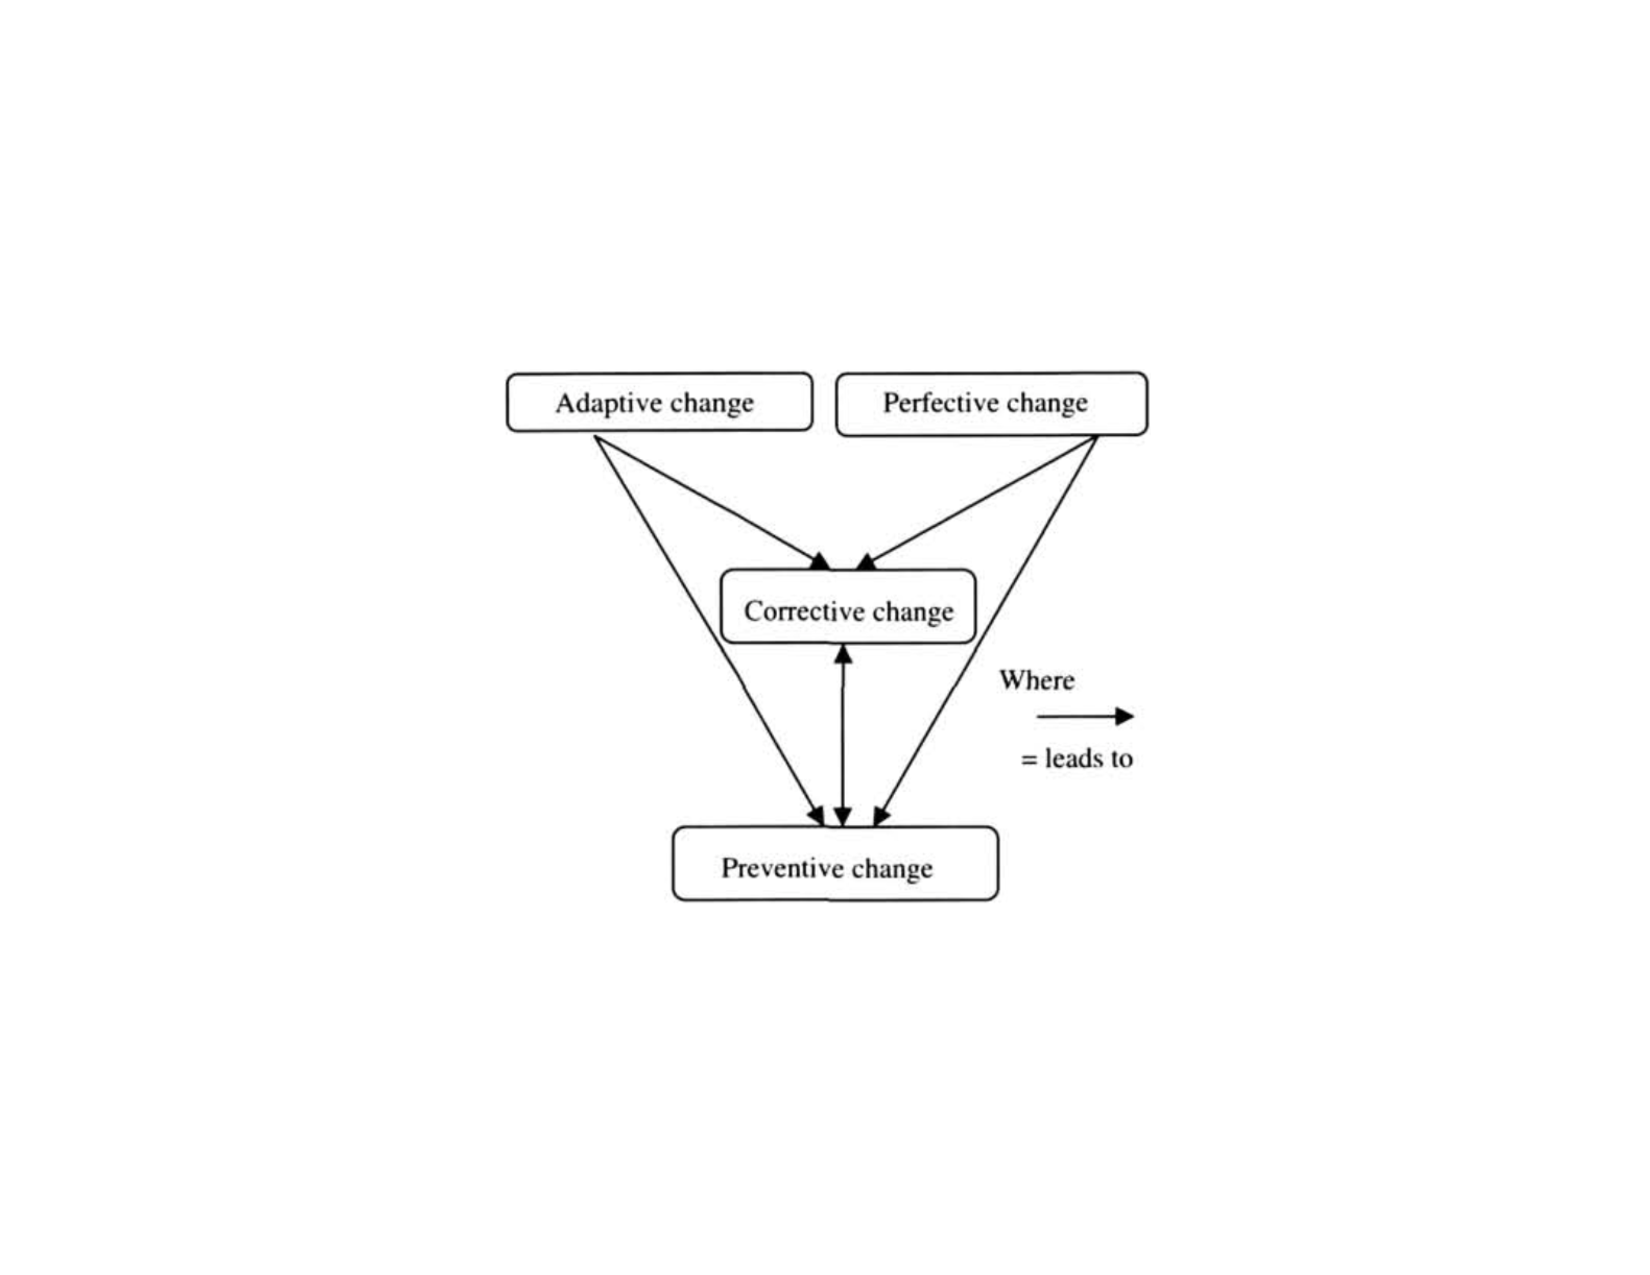
\includegraphics{images/relationship_of_changes.pdf}}
\caption{Potential relation between software changes~\cite{Seaman2008:SMC}}
\label{fig:relation}
\end{figure}

Figure~\ref{fig:relation} presents the potential relationships between different types of changes~\cite{Seaman2008:SMC}. Specifically, both adaptive changes and perfective changes may lead to the other two types of changes, because developers may introduce bugs or worsen code structures when adapting software to new environments or implementing new features.



\section{An Organized Tour of Seminal Papers: I. Applying Changes}
\label{sec:apply}

We discuss the characteristics of {\em corrective}, {\em adaptive}, {\em perfective}, and {\em preventative} changes using empirical studies and the process and techniques for applying software changes, respectively in Sections~\ref{sec:corrective},~\ref{sec:adaptive},~\ref{sec:perfective}, and~\ref{sec:preventive}. Next, regardless of change types, automation could reduce the manual effort of applying software changes. Therefore, we discuss the topic of automated program transformation and editing techniques for reducing repetitive edits in Section~\ref{sec:automatic}.

\subsection{Corrective Change}
\label{sec:corrective}
\newtext{Corrective changes such as bug fixes are frequently applied by developers to eliminate defects in software. There are mainly two lines of research conducted: (1) empirical studies to characterize bugs and corresponding fixes, and (2) automatic approaches to detect and fix such bugs. There is no clear boundary between the two lines of research, because some prior projects first make observations about particular kinds of bug fixes empirically and then subsequently leverage their observed characteristics to find more bugs and fix them. Below, we discuss a few representative examples of empirical studies with such flavor of characterizing existing bugs and fixing them.} 
%~\cite{Fenton2000:QAF,Li2006:TCE,Kim2006:MBF,Lu2008:LMC,Nguyen2010:RBF,Yin2011:FBB,Park2012:supplementary,Zhong2015:ESR}
% ~\cite{Engler2000:CSR,Bush2000:SAF,Hangal2002:TDS,Hovemeyer2004:FBE,Naik2006:ESR,Weimer2009:AFP}. 
% ~\cite{Li2006:CPMiner,Pham2010:DRS,Jin2012:UDR,Kim2013:PAR} 

 
\subsubsection{Empirical Studies of Bug Fixes.}
\newtext{In this section, we discuss two representative studies on bug fixes. These studies are not the earliest, seminal works in this domain. Rather, the flavor and style of their empirical studies is representative. Li et al. conducted is a large scale characterization of bugs by digging through bug reports in the wild and by quantifying the extent of each bug type~\cite{Li2006:TCE}. S. Kim et al.'s {\em memory of bug fixes}~\cite{Kim2006:MBF} uses fine-grained bug fix histories to measure the extent of recurring, similar bug fixes and to assess the potential of automating similar fixes based on change history. } 

% write studies with past tense 

\newtext{Li et al.~conducted an empirical study of bugs from two popular open source projects: Mozilla and Apache HTTP Server~\cite{Li2006:TCE}. By manually examining 264 bug reports from the Mozilla Bugzilla database, and 209 bug reports from the Apache Bugzilla database, they investigated the root cause, impact, and software components of each software error that exhibited abnormal runtime behaviors. They observed three major root causes: {\em memory}, {\em concurrency}, and {\em semantics}. The memory bugs accounted for 16.3\% in Mozilla and 12.2\% in Apache. Among memory bugs, NULL pointer dereference was observed as a major cause, accounting for 37.2\% in Mozilla and 41.7\% in Apache. More importantly, semantic bugs were observed to be dominant, accounting for 81.1\% in Mozilla and 86.7\% in Apache. One possible reason is that most semantic bugs are specific to applications. A developer could easily introduce semantic bugs while coding, due to a lack of thorough understanding of software and its requirements. It is challenging to automatically detect or fix such semantic bugs, because diagnosing and resolving them may require a lot of domain-specific knowledge and such knowledge is inherently not generalizable across different systems and applications. } 

To understand the characteristics and frequency of project-specific bug fixes, Kim et al.~conducted an empirical study on the bug fix history of five open source projects: ArgoUML, Columba, Eclipse, jEdit, and Scarab~\cite{Kim2006:MBF}. With keywords like ``Fixed'' or ``Bugs'', they retrieved code commits in software version history that are relevant to bug fixes, chopped each commit into contiguous code change blocks (i.e., hunks), and then clustered similar code changes. They observed that 19.3 to 40.3\% bugs appeared repeatedly in version history, while 7.9 to 15.5\% of bug-and-fix pairs appeared more than once.
\newtext{The results demonstrated that project-specific bug fix patterns occur frequently enough and for each bug-and-fix pair, it is possible to both detect similar bugs and provide fix suggestions. The study also showed history-based bug detection could be complementary to static analysis-based bug detection\textemdash the bugs that can be detected by past bug fix histories do not overlap with the bugs that can be detected by a static bug finding tool, PMD~\cite{PMD}.}

\subsubsection{Rule-based Bug Detection and Fixing Approaches.}
Rule-based bug detection approaches detect and fix bugs based on the assumption that bugs are {\em deviant program behaviors} that violate implicit programming rules. Then one may ask, where those implicit rules are coming from? Such rules can be written by the developers of bug-finding tools or can be refined based on empirical observation in the wild. For example, Engler et al.~define a meta-language for users to easily specify temporal system rules such as ``release locks after acquiring them''~\cite{Engler2000:CSR}. They also extend a compiler to interpret the rules and dynamically generate additional checks in the compiler. If any code snippet violates the specified rule(s), the approach reports the snippet as a software bug. Table~\ref{tab:rule} presents some exemplar system rule templates and instances. With this approach, developers can flexibly define their own rules to avoid some project-specific bugs, without worrying how to implement checkers to enforce the rules. Engler et al.'s later work enables tool developers to tailor rule templates to a specific system and checks for contradictions and violations\cite{engler01bugs}.  

\begin{table}[]
\centering
\caption{Sample system rule templates and examples from~\cite{Engler2000:CSR}}
\label{tab:rule}
\begin{tabular}{l|l}
\toprule
Rule template                  & Example                                                 \\ \hline
``Never/always do X''          & ``Do not use floating point in the kernel''             \\\hline
``Do X rather than Y''         & ``Use memory mapped I/O rather than copying''           \\ \hline
``Always do X before/after Y'' & ``Check user pointers before using them in the kernel''\\
\bottomrule
\end{tabular}
\end{table} 

As another example of rule-based bug detection is CP-Miner, an automatic approach to find copy-paste bugs in large-scale software~\cite{Li2006:CPMiner}. CP-Miner is motivated by Chou et al.'s finding that, under the Linux {\sf drivers/i2o} directory, 34 out of 35 errors were caused by copy-paste~\cite{Chou2001:ESO} and based on the insight that when developers copy and paste, they may forget to consistently rename identifiers. CP-Miner first identifies copy-paste code in a scalable way, and then detects bugs by checking for such specific rules, for example, consistent renaming of identifiers. %Many previously unknown bugs in popular operating systems were detected in this way, 49 in Linux and 31 in FreeBSD, meaning that CP-Miner can effectively capture copy-paste related bugs. 
%Similarly, FixWizard identifies code clones based on object usage and interactions, recognizes recurring bug-fixes to the clones, and suggests a location and example edit~\cite{Nguyen2010:RBF}. However, it does not generate fixes.
\subsubsection{Automated Repair.} 
Automatic program repair generates candidate patches and checks correctness using compilation, testing, and/or specification. 

\newtext{One set of techniques uses {\em search-based repair}~\cite{harman07} or predefined repair templates to generate many candidate repairs for a bug, and then validates them using indicative workloads or test suites. For example, GenProg generates candidate patches by replicating, mutating, or deleting code \emph{randomly} from the existing program~\cite{genprog-icse2012, Weimer2009:AFP}. GenProg uses genetic programming (GP) to search for a program variant that retains required functionality but is not vulnerable to the defect in question. GP is a stochastic search method inspired by biological evolution that discovers computer programs tailored to a particular task. GP uses computational analogs of biological mutation and crossover to generate new program variations, in other words, program variants. A user-defined fitness function evaluates each variant. GenProg uses the input test cases to evaluate the fitness, and individuals with high fitness are selected for continued evolution. This GP process is successful, when it produces a variant that passes all tests encoding the required behavior and does not fail those encoding the bug.}

%Many of these approaches can scale to repair defects in large systems with human-competitive costs. However, they tend to find the smallest possible fix for a given failure, and current evidence suggests that humans may find the resulting patches unacceptable in many cases~\cite{genprog-maintainability,Kim2013:PAR}. 

\newtext{Another class of strategies in automatic software repair relies on {\em specifications} or {\em contracts} to guide sound patch generation. %\cite{gopinath2011, liblit2011, liu2012, semfix13,Wei:2010:AutoFix-E}. 
This provides confidence that the output is correct. For example, AutoFix-E generates simple bug fixes from manually prescribed contracts~\cite{Wei:2010:AutoFix-E}. The key insights behind this approach are to rely on contracts present in the software to ensure that the proposed fixes are semantically sound. AutoFix-E takes an Eiffel class and generates test cases with some automated testing engine first. From the test runs, it extracts object states using boolean queries. By comparing the states of passing and failing runs, it then generates a fault profile\textemdash an indication of what went wrong in terms of an abstract object state. From the state transitions in passing runs, it generates a finite-state behavioral model, capturing the normal behavior in terms of control. Both control and state guide the generation of fix candidates, and only those fixes passing the regression test suite remain.}

% Genetic programming has also been used to co-evolve defect repairs and unit test cases~\cite{Arcuri11,wilkerson2012}; these techniques tend to rely at least in part on formal specifications to define correctness~\cite{arcuriy08,wilkerson11}.  Such techniques struggle to scale, and are usually limited to manually specified code, which is rare in practice.

	Some approaches are specialized for particular types of bugs only. For example, FixMeUp inserts missing security checks inter-procedurally using a specification, but these additions are very specific and stylized for access-control related security bugs~\cite{son2013fix}. As another example, PAR~\cite{Kim2013:PAR} encodes ten common bug fix patterns from Eclipse JDT's version history to improve GenProg. However, the patterns are created manually.
%Given concurrency error reports, Jin et al.~select from and test a handful of synchronization patterns to fix them~\cite{JZDLL:12} and insert appropriate synchronization into a compiler intermediate representation. 

 

\subsection{Adaptive Change}
\label{sec:adaptive}
Adaptive changes are applied to software, when its environment changes. In this section, we focus on three scenarios of adaptive changes: cross-system software porting, cross-language software migration, and software library upgrade (i.e., API evolution).

Consider an example of cross-system porting. When a software system is installed on a computer, the installation can depend on configurations of the hardware, the software, and the device drivers for particular devices. To make the software to run on a different processor or a operating system, and to make it compatible with different drivers, we may need adaptive changes to adjust the software to the new environment. 
Consider another example of cross-language migration where you have software in Java that must be translated to Java. Developers need to rewrite software and must also update language-specific libraries.
Finally consider the example of API evolution. When the APIs of a library and a platform evolves, corresponding adaptations are often required for client applications to handle such API update. In extreme cases, e.g., when porting a Java desktop application to the iOS platform, developers need to rewrite everything from scratch, because both the programming language (i.e., Swift) and software libraries are different. 

\subsubsection{Cross-System Porting.} 
Software forking\textemdash creating a variant product by copying and modifying an existing product\textemdash is often considered an ad hoc, low cost alternative to principled product line development. To maintain such forked products, developers often need to port an existing feature or bug-fix from one product variant to another. 

\paragraph{{Empirical Studies on Cross-System Porting.}}
As OpenBSD, NetBSD, and FreeBSD have evolved from the same origin but been maintained independently from one another, many have studied the BSD family to investigate the extent and nature of cross-system porting. For example, Fischer et al.~analyzed change commit messages of the BSD family and found a decreasing trend of information flow between OpenBSD and other BSD projects~\cite{Fischer2005}. Yamamoto et al.~found that up to 40\% of lines of code were shared among NetBSD, OpenBSD, and FreeBSD~\cite{Yamamoto2005}. James et al.~showed the evidence of adopted code in device driver modules between Linux and FreeBSD~\cite{Cordy2011:largecloning}. Canfora et al.~investigated the social characteristics of contributors who made cross-system bug fixes between FreeBSD and OpenBSD~\cite{Canfora2011:bsdfork} by using textual analysis of change commit logs and mailing list communication logs. They observed that contributors who port changes from other projects are highly active contributors. Ozment et al.~investigated security vulnerabilities in the OpenBSD project to examine whether software security improves with age~\cite{Ozment2006}. Ray et al.~comprehensively characterized the temporal, spatial, and developer dimensions of cross-system porting in the BSD family. Their study found that maintaining forked projects involves significant effort of porting patches from other projects and that cross-system porting  is periodic and its rate does not necessarily decrease over time~\cite{Ray2012:FSE}. %A significant portion of active developers participate in porting changes from peer projects. Ported changes are less defect-prone than non-ported changes. 

\paragraph{{Cross-Platform Software Development.}}
When assigning different software development teams to independently work on separate source trees targeting different platforms, different teams maintain almost identical functionality and incur redundant effort. Some programming languages (e.g., 8th~\cite{8th}), software libraries (e.g., cairo~\cite{cairo}) and frameworks (e.g.,Ultimate++~\cite{ultimate}) are built to facilitate cross-platform software development. With such tool support, developers only need to build software once, but generate executable software for multiple platforms. % In particular, HTML5 is designed to deliver almost everything customers may need without requiring additional software (e.g., browser plugins) to install~\cite{html5}. 
To simplify cross-platform mobile software development, existing tools support developers to write code in HTML5 (e.g., Sencha~\cite{sencha}), or even automatically translate HTML5 implementation to Android or iOS native code (e.g., PhoneGap~\cite{phonegap}).

\subsubsection{Cross-Language Migration.} 
When maintaining a legacy system that was written in an old programming language (e.g., Fortran) decades ago, programmers may migrate the system to a mainstream general-purpose language, such as Java, to facilitate the maintenance of existing codebase and to extend the system by leveraging new programming language features. 
%Different from the API adaptive changes mentioned above, such software translation requires of a significant amount of coding effort to rewrite the same application in a new programming language.
%\todo{Na, more techniques? I think this section is relatively weaker than others. I also do not think we can talk about TXL here, since we decided to talk about automated techniques separately.} 

\paragraph{{Cross-Language Program Translation.}}
To translate code implementation from one language to another, researchers have built tools by hard coding the translation rules and implementing any missing functionality between languages~\cite{Yasumatsu:95,1192409:03,Sneed:2010}. 
%SPiCE translates Smalltalk programs into a C environment by mapping the execution models of two languages. Specifically, 
Yasumatsu et al.~map compiled methods and contexts in Smalltalk to machine code and stack frames respectively, and implement runtime replacement classes in correspondence with the Smalltalk execution model and runtime system~\cite{Yasumatsu:95}. Mossienko~\cite{1192409:03} and Sneed~\cite{Sneed:2010} automate COBOL-to-Java code migration by defining and implementing rules to generate Java classes, methods, and packages from COBOL programs. 
{\em mppSMT} automatically infers and applies Java-to-C\# migration rules using a phrase-based statistical machine translation approach~\cite{7372046}. It encodes both Java and C\# source files into sequences of syntactic symbols, called {\em syntaxemes}, and then relies on the syntaxemes to align code and to train sequence-to-sequence translation. 

\paragraph{{Mining Cross-Language API Rules.}}
When migrating software to a different target language, API conversion poses a challenge for developers, because the diverse usage of API libraries induces an endless process of specifying API translation rules or identifying API mappings across different languages. Zhong et al.~\cite{zhong2010mining} and Nguyen et al.~\cite{nguyen2014statistical,Nguyen:2017:EAE} automatically mine API usage mappings between Java and C\#. Zhong et al.~align code based on similar names, and then construct the API transformation graphs for each pair of aligned statements~\cite{zhong2010mining}. StaMiner~\cite{nguyen2014statistical} mines API usage sequence mappings by conducting program dependency analysis~\cite{Muchnick:1998} and representing API usage as a graph-based model~\cite{Nguyen09}. %API2VEC mine API usage sequence mappings by converting API element sequences to vectors, and comparing cosine similarities between vectors~\cite{Nguyen:2017:EAE}. 

\subsubsection{Library Upgrade and API Evolution.}
Instead of building software from scratch, developers often use existing frameworks or third-party libraries to reuse well-implemented and tested functionality. Ideally, the APIs (Application Programming Interfaces) of libraries must remain stable such that library upgrades do not incur corresponding changes in client applications. In reality, however, APIs change their input and output signatures, change semantics, or are even deprecated, forcing client application developers to make corresponding adaptive changes in their applications.  

\paragraph{{Empirical Studies of API Evolution.}}
Dig and Johnson manually investigated API changes using the change logs and release notes to study the types of library-side updates that break compatibility with existing client code, and discovered that 80\% of such changes are refactorings~\cite{Dig2005}. Xing and Stroulia used UMLDiff to study API evolution and found that about 70\% of structural changes are refactorings~\cite{Xing2006:apievol}. Yokomori et al. investigated the impact of library evolution on client code applications using component ranking measurements~\cite{Yokomori2009:apiimpact}. Padioleau et al. found that API changes in the Linux kernel led to subsequent changes on dependent drivers, and such collateral evolution could introduce bugs into previously mature code~\cite{Padioleau2006:collateral}. McDonelle et al. examined the relationship between API stability and the degree of adoption measured in propagation and lagging time in the Android Ecosystem~\cite{McDonnell2013:api}. Hou and Yao studied the Java API documentation and found that a stable architecture played an important role in supporting the smooth evolution of the AWT/Swing API~\cite{Hou2011:api}. In a large scale study of the Smalltalk development communities, Robbes et al.~found that only 14\% of deprecated methods produce non-trivial API change effects in at least one client-side project; however, these effects vary greatly in magnitude. On average, a single API deprecation resulted in 5 broken projects, while the largest caused 79 projects and 132 packages to break~\cite{robbes2012}.

\paragraph{{Tool Support for API Evolution and Client Adaptation.}} 
Several existing approaches semi-automate or automate client adaptations to cope with evolving libraries.  Chow and Notkin~\cite{Chow1996} propose a method for changing client applications in response to library changes\textemdash a library maintainer annotates changed functions with rules that are used to generate tools that update client applications. Henkel and Diwan's CatchUp records and stores refactorings in an XML file that can be replayed to update client code~\cite{Henkel2005}. However, its update support is limited to three refactorings: renaming operations (e.g.  types, methods, fields), moving operations (e.g. classes to different packages, static members), or change operations (e.g. types, signatures). The key idea of CatchUp, {\em record-and-replay}, assumes that the adaptation changes in client code are exact or similar to the changes in the library side. Thus, it works well for replaying rename or move refactorings or supporting API usage adaptations via inheritance. However, CatchUp cannot suggest programmers how to manipulate the context of API usages in client code such as the surrounding control structure or the ordering between method-calls. Furthermore, CatchUp requires that library and client application developers use the same development environment to record API-level refactorings, limiting its adoption in practice. Xing and Stroulia's Diff-CatchU automatically recognizes API changes of the reused framework and suggests plausible replacements to the obsolete APIs based on the working examples of the framework codebasep~\cite{Xing2007:diffcatchup}. Dig et al.'s MolhadoRef uses recorded API-level refactorings to resolve merge conflicts that stem from refactorings; this technique can be used for adapting client applications in case of simple rename and move refactorings occurred in a library~\cite{Dig2007}.  

SemDiff~\cite{Dagenais2008:RAC} mines API usage changes from other client applications or the library itself.  It defines an adaptation pattern as a frequent {\em replacement} of a method invocation. That is, if a method call to $A.m$ is changed to $B.n$ in several adaptations, $B.n$ is likely to be a correct replacement for the calls to $A.m$. As SemDiff models API usages in terms of method calls, it cannot support complex adaptations involving multiple objects and method calls that require the knowledge of the surrounding context of those calls. LibSync helps client applications migrate library API usages by learning migration patterns~\cite{Nguyen2010:GAA} with respect to a partial AST with containment and data dependences. Though it suggests what code locations to examine and shows example API updates, it is {unable} to transform code automatically. Cossette and Walker found that, while most broken code may be mended using one or more of these techniques, each is ineffective when used in isolation~\cite{cossette2012}. 

\paragraph{{API Usage Specification Extraction.}} 
Several approaches extract API usage specifications from existing code. The forms of recovered API usage specifications and patterns include finite state automaton~\cite{zeller07,doc2spec}, pairs of method calls~\cite{Livshits2005,williams-tse05}, partial orders of calls~\cite{mapo-fse07,taoxie-ase09}, and Computation Tree Logic formulas~\cite{zeller-ase09}. The API usage representations in those static approaches are still limited, for example, the patterns are without control structures and involve only individual objects belonging to one class. In contrast to those static approaches, dynamic approaches recover the specifications by investigating the execution traces of programs but they require a huge amount of execution traces.  
%\cite{javert,perracotta,shoham-issta07,ramanathan-isce07,mike-ase09}


 
 

\subsection{Perfective Change}
\label{sec:perfective}
Perfective change is the change undertaken to expand the existing requirements of a system. Not much research is done to characterize feature enhancement or addition. One possible reason is that the implementation logic is always domain and project-specific and that it is challenging for any automatic tool to predict what new feature to add and how that new feature must be implemented. Therefore, the nature and characteristics of feature additions are under-studied. 

In this section, we discuss a rather well-understood type of perfective changes, called {\em crosscutting concerns} and techniques for implementing and managing crosscutting concerns. As programs evolve over time, they may suffer from the {\it the tyranny of dominant decomposition}~\cite{Tarr1999}. They can be modularized in only one way at a time. Concerns that are added later may end up being scattered across many modules and tangled with one another. Logging, performance, error handling, and synchronization are canonical examples of such secondary design decisions that lead to non-localized changes.
  
Aspect-oriented programming languages provide language constructs to allow concerns to be updated in a modular fashion~\cite{Kiczales2001:OA}. Other approaches instead leave the crosscutting concerns in a program, while providing mechanisms to document and manage related but dispersed code fragments. For example, Griswold's information transparency technique uses naming conventions, formatting styles, and ordering of code in a file to provide indications about crosscutting concern code that should change together \cite{Griswold2001}. 

\subsubsection{Techniques for Locating Crosscutting Concerns.}
Several tools allow programmers to automatically or semi-automatically locate crosscutting concerns. Robillard et al. allow programmers to manually document crosscutting concerns using structural dependencies in code~\cite{Robillard2003}. Similarly, the Concern Manipulation Environment allows programmers to locate and document different types of concerns~\cite{Harrison2005}. Van Engelen et al. use clone detectors to locate crosscutting concerns~\cite{VanEngelen2005}. Shepherd et al. locate concerns using natural language program analysis~\cite{Shepherd2007}. Breu et al.~mine aspects from version history by grouping method-calls that are added together~\cite{Breu2006}. Dagenais et al.~automatically infer and represent structural patterns among the participants of the same concern as rules in order to trace the concerns over program versions~\cite{Dagenais2007}. 

\subsubsection{Language Support for Crosscutting Concerns.}
{\it Aspect-Oriented Programming} (AOP) is a programming paradigm that aims to increase modularity by allowing the separation of crosscutting concerns~\cite{aspectj}. Suppose developers want to add a new feature such as logging to log all executed functions. The logging logic is straightforward: printing the function's name at each function's entry. However, manually inserting the same implementation to each function body is tedious and error-prone. With AOP, developers only need to first define the logging logic as \textbf{an advice}, and then specify the place where to insert the advice (i.e., \textbf{pointcut}), such as the entry point of each function. An aspect weaver will read the aspect-oriented code, and generate appropriate object-oriented code with the aspects integrated. In this way, AOP facilitates developers to efficiently introduce new program behaviors without cluttering the core implementation in the existing codebase. Many Java bytecode manipulation frameworks implement the AOP paradigm, like ASM~\cite{asm}, Javassist~\cite{javassist}, and AspectJ~\cite{aspectj}, so that developers can easily modify program runtime behaviors without touching source code. The benefit of AOP during software evolution is that crosscutting concerns can be contained as a separate module such as an {\tt aspect} with its {\tt pointcut} and {\tt advice} description, and thus reduces the developer effort in locating and updating all code fragments relevant to a particular secondary design decision such as logging, synchronization, database transaction, etc. 

{\it Feature Oriented Programming} (FOP) is another paradigm for program generation in software product lines and for incremental development of programs~\cite{Batory1992:DIH}. FOP is closely related to AOP. Both deal with modules that encapsulate crosscuts of classes, and both express program extensions. In FOP, every software is considered as a composition of multiple features or layers. Each feature implements a certain program functionality, while features may interact with each other to collaboratively provide a larger functionality. A software product line (SPL) is a family of programs where each program is defined by a unique composition of features. Formally, FOP considers programs as \emph{values} and program extensions as \emph{functions}~\cite{Lammel2013:fop}. The benefit of FOP is similar to AOP in that secondary design decisions can be encapsulated as a separate feature and can be composed later with other features using program synthesis, making it easier to add a new feature at a later time during software evolution. Further discussion of program generation techniques for software product lines is described elsewhere in Chapter~\todo{cross reference a chapter on the product line}.  
  
\begin{comment} 
\noindent Suppose there are two programs: \\
$f\text{	// program with feature }f$, and\\
$g\text{	// program with feature }g$.\\
A program extension is a function that takes a program as input and produces a feature-augmented program output. Suppose there are two program extensions:\\
$i \bullet x$ \text{// adds feature i to program x}, and \\
$j \bullet y$ \text{// adds feature j to program y}.\\
By applying the functions to the values, we can compose more than one multi-featured application as below:
$app1 = i \bullet f$ // \text{app1 has features i and f},\\
$app2 = j \bullet g$ // \text{app2 has features j and g}, and\\ 
$app3 = i \bullet j \bullet f$ // \text{app3 has features i, j, and f}.
\end{comment} 
 

 

\subsection{Preventive Change}
\label{sec:preventive}
As a software system is enhanced, modified, and adapted to new requirements, the code becomes more complex and drifts away from its original design, thereby lowering the quality of the software. {\em Refactoring}~\cite{1999:RID,Griswold:1992,Opdyke1992:ROF,Mens2004:SSR} copes with increasing software complexity by transforming a program from one representation to another while preserving the program's external behavior (functionality and semantics).

Mens et al.~present a survey of refactoring research and describe a refactoring process, consisting of the following activities~\cite{Mens2004:SSR}:
\begin{enumerate}
\item Identifying where to apply what refactoring(s).
\item Checking that the refactoring to apply preserves program behaviors.
\item Refactoring the code.
\item Assessing the effect of applied refactoring on software quality (e.g., complexity and readability). 
\item Maintaining the consistency between refactored code and other related software artifacts, like documentation, tests, and issue tracking records.  
\end{enumerate}

Section~\ref{sec:refactoringdefinition} describes the definition of refactoring and example transformations and Section~\ref{sec:refactoringstudies} describes empirical studies on refactoring. Section~\ref{sec:automatedrefactoring} describes tool support for automated refactoring. Section~\ref{sec:refactoringpractice} describes several studies of modern refactoring practices and the limitations of current refactoring support. Section~\ref{sec:refactoringassessment} describes techniques for assessing the impact of refactoring. Section~\ref{sec:codesmell} describes techniques for identifying opportunities for refactoring. 

\subsubsection{Definition of Refactoring Operations.} 
\label{sec:refactoringdefinition} 

Griswold's dissertation \cite{Griswold:1992} discusses one of the first refactoring operations that automate repetitive, error-prone, non-local transformations. Griswold supports a number of restructuring operations: replacing an expression with a variable that has its value, swapping the formal parameters in a procedure's interface and the respective arguments in its calls, etc. It is important to note that many of these refactoring operations are systematic in the sense that they involve repetitive non-local transformations. 

Opdyke's dissertation \cite{Opdyke1992:ROF} distinguishes the notion of low-level refactorings from high-level refactorings. High-level refactorings (i.e., composite refactorings) reflect more complex behavior-preserving transformations while low-level refactorings are primitive operations such as creating, deleting, or changing a program entity or moving a member variable. Opdyke describes three kinds of complex refactorings in detail: (1) creating an abstract superclass, (2) subclassing and simplifying conditionals, and (3) capturing aggregations and components. All three refactorings are systematic in the sense that they contain multiple similar transformations at a code level. For example, {creating an abstract superclass} involves moving multiple variables and functions common to more than one sibling classes to their common superclass.  {Subclassing and simplifying conditionals} consists of creating  several classes, each of which is in charge of evaluating a different conditional. Capturing aggregations and components usually involves moving {multiple} members from a component to an aggregate object. 

While refactoring is defined as behavior-preserving code transformations in the academic literature~\cite{Mens2004:SSR}, the de-facto definition of refactoring in practice seems to be very different from such rigorous definition. Fowler catalogs 72 types of structural changes in object oriented programs but these transformations do not necessarily guarantee behavior preservation~\cite{1999:RID}. In fact, Fowler recommends developers to write test code first before, since these refactorings may change a program's behavior. Murphy-Hill et al.~analyzed refactoring logs and found that developers often interleave refactorings with other behavior-modifying transformations~\cite{Murphy-Hill2012:refactor}, indicating that pure refactoring revisions are rare. Johnson's refactoring definition is aligned with these findings\textemdash{\it refactoring improves behavior in some aspects but does not necessarily preserve behavior in all aspects}~\cite{Johnson2011}.

\subsubsection{Empirical Studies of Refactoring.} 
\label{sec:refactoringstudies} 

Hindle et al. found that large commits are more refactorings, while small commits are more bug fixes~\cite{Hindle2008:largecommit}. Purushothaman and Perry found that nearly 10\% of changes involved only a single line of code, which has less than a 4\% chance to result in error, while a change of 500 lines or more has nearly a 50\% chance of causing at least one defect. This result may indicate that large commits, which tend to include refactorings, have a higher chance of inducing bugs. 

Wei{\ss}gerber and Diehl found that refactorings often occur together with other types of changes and that refactorings are followed by an increasing number of bugs~\cite{Weissgerber2006:refactor}. Carriere et al.'s case study found that the productivity measure manifested by the average time taken to resolve tickets decreases after re-architecting the system~\cite{Carriere2010:architecture}. Ratzinger et al.~developed defect prediction models based on software evolution attributes and found that refactoring related features and defects have an inverse correlation~\cite{Ratzinger2008:refactor}\textemdash if the number of refactorings increases in the preceding time period, the number of defects decreases. Kim et al.~\cite{Kim2011:refactorbug} investigated the spatial and temporal relationship between API refactorings and bug fixes using a K-revision sliding window and by reasoning about the method-level location of refactorings and bug fixes. They found that the number of bug fixes increases after API refactorings~\cite{Kim2011:refactorbug}.  

Though the intent of refactoring is to improve software maintainability, refactoring could be potentially error-prone as it often requires coordinated edits across different parts of a system. Several researchers found such evidence from open source project histories\textemdash M. Kim et.al.'s program differencing technique~\cite{Kim2007,Kim:2009} identifies exceptions to systematic change patterns, which often arise from the failure to complete coordinated refactorings. G{\"o}rg and Wei{\ss}gerber detect errors caused by incomplete refactorings by relating API-level refactorings to the corresponding class hierarchy~\cite{Gorg2005a}. Nagappan and Ball found that code churn\textemdash the number of added, deleted, and modified lines of code\textemdash is correlated with defect density~\cite{Nagappan2005}\textemdash since refactoring often introduces a large amount of structural changes to the system, some question the benefit of refactoring. 

\subsubsection{Automated Refactoring.} 
\label{sec:automatedrefactoring} 

The Eclipse IDE provides automatic support for a variety of refactorings, including \emph{rename}, \emph{move}, and \emph{extractMethod}. With such support, developers do not need to worry about how to check for preconditions or postconditions before manually applying a certain refactoring. Instead, they can simply select the refactoring command from a menu (e.g., \emph{extractMethod}), and provide necessary information to accomplish the refactoring (e.g., \emph{the name of a new method}). The Eclipse refactoring engine takes care of the precondition check, program transformation, and postcondition check. 

During refactoring automation, Opdyke suggests to ensure behavior preservation by specifying \emph{refactoring preconditions}~\cite{Opdyke1992:ROF}. For instance, when conducting an \emph{create\_method\_function} refactoring, before inserting a member function $F$ to a class $C$, developers should specify and check for five preconditions, as shown in Figure~\ref{fig:preconditions}. If any precondition is not satisfied, the refactoring should not be applied to the program.

\begin{figure}[!htb]
\centering
\scalebox{0.55}{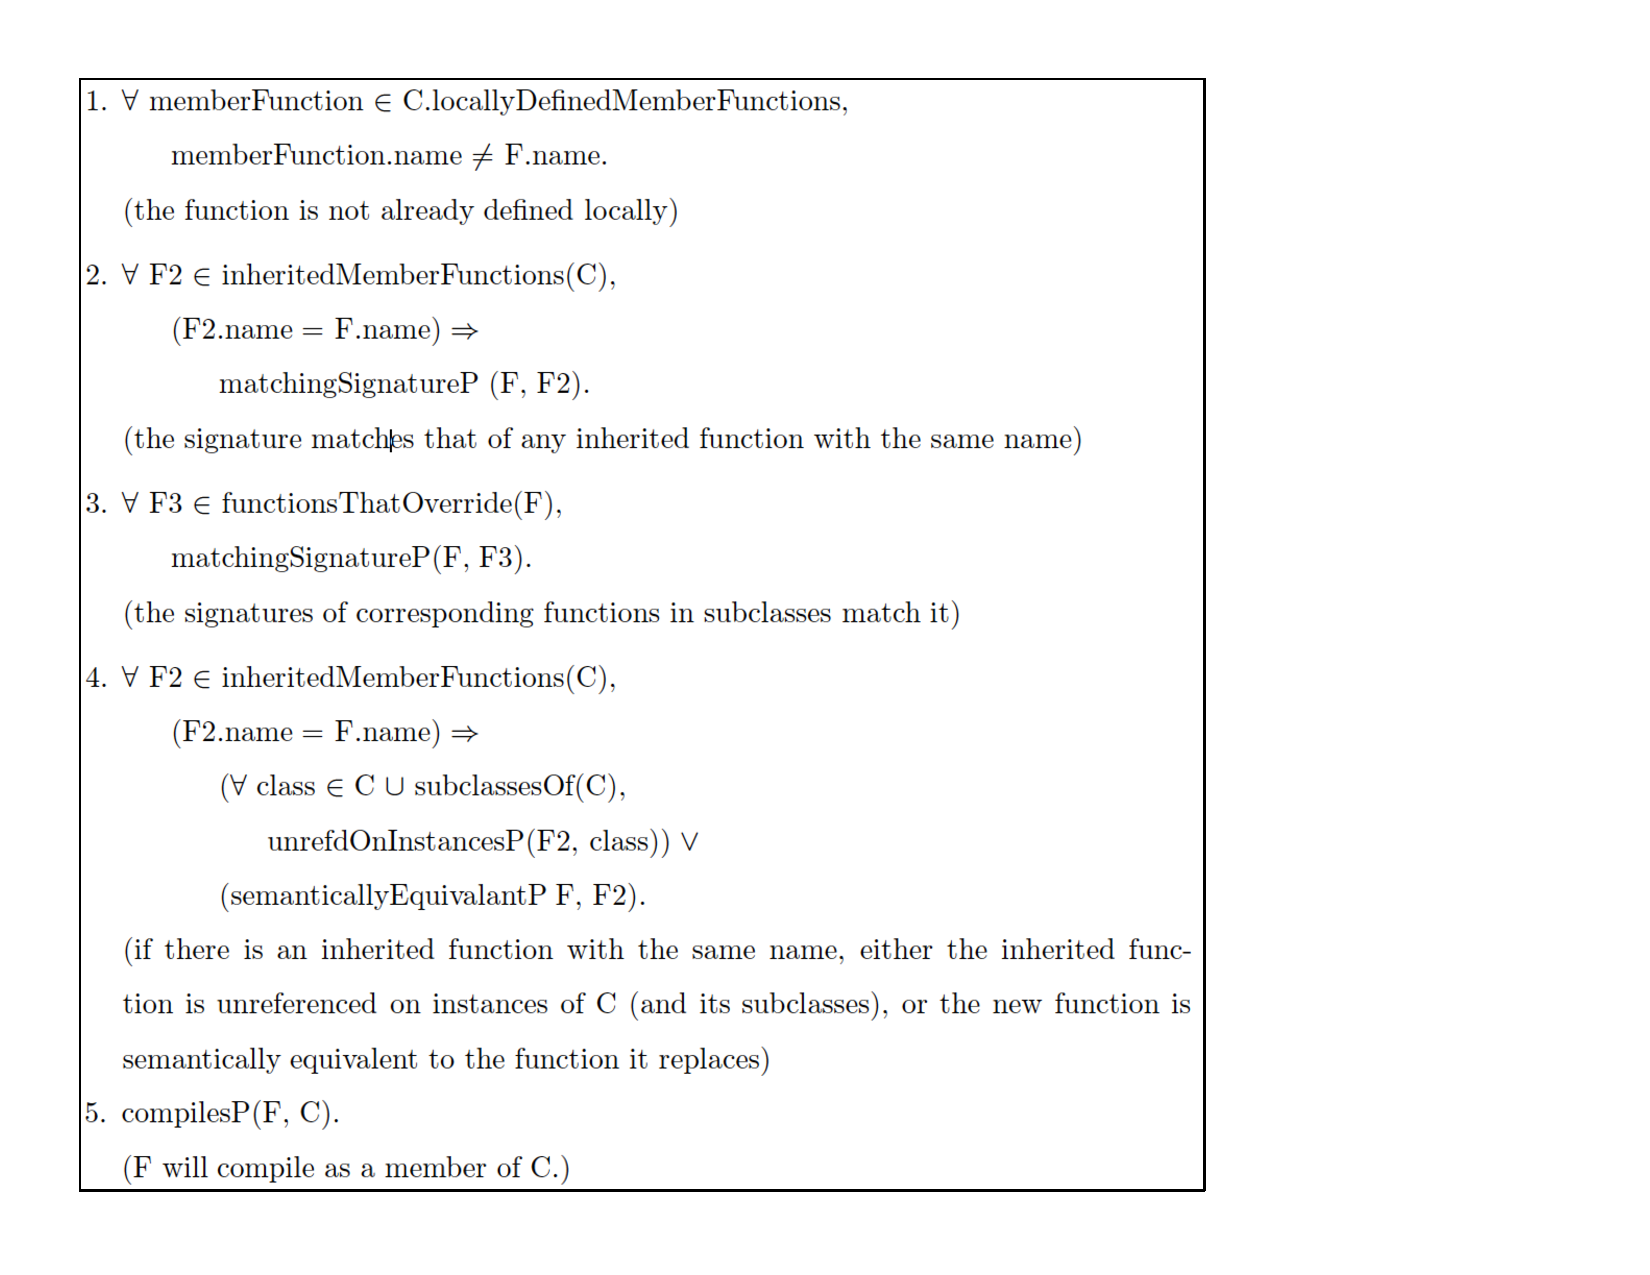
\includegraphics{images/preconditions.pdf}}
\caption{Preconditions for \emph{create\_method\_function} refactoring~\cite{Opdyke1992:ROF}}
\label{fig:preconditions}
\end{figure}

%Additionally, researchers conducted empirical studies to characterize the refactorings applied by developers~\cite{Kim2012:FSR,Murphy-Hill2012:refactor,Vakilian:2012,Silva2016:WWR}, and proposed various approaches to automate refactoring or to complete the refactoring tasks initiated by developers~\cite{Griswold:1992,Balazinska1999,Dig:2009,Ge:2012,Chen:2013,Lee:2013,Tsantalis2013:icsm,Meng2015:ARO,Kim:2016}. For instance, Silva et al.~observed that refactoring activity is mainly driven by changes in the requirements and much less by code smells~\cite{Silva2016:WWR}. Kim et al.~developed R3, an alternative refactoring engine that works 10 times faster than Eclipse Refactoring~\cite{Kim:2016}. 

%Based on code clones detected by various techniques~\cite{Kamiya2002,Jiang2007a,Krinke2001:PDG}, many tools identify or rank refactoring opportunities~\cite{Balazinska1999a, Higo2008:metricrefactoring, goto2013extract, higo2013identifying, Tsantalis2011:rankRefactoring}. For instance, Balazinska et al.~\cite{Balazinska1999a} define a clone classification scheme based on various types of differences between clones and automate the classification to help developers assess refactoring opportunities for each clone group. Higo et al.~and Goto et al.\/ rank clones as refactoring candidates based on coupling or cohesion metrics~\cite{Higo2008:metricrefactoring,goto2013extract}. Others integrate evolution information in software history to rank clones that have been repetitively or simultaneously changed in the past~\cite{higo2013identifying, Tsantalis2011:rankRefactoring}. While these tools detect refactoring opportunities for clones, they do not automatically refactor code.
A number of techniques automate clone removal refactorings by factorizing the common parts and by parameterizing their differences using a {\em strategy} design pattern or a {\em form template method} refactoring~\cite{Balazinska1999, tairas2012increasing, juillerat2007toward, hotta2012identifying, Tsantalis2013:icsm}. These tools insert customized calls in each original location to use newly created methods. Juillerat et al.~automate {\em introduce exit label} and {\em introduce return object} refactorings~\cite{juillerat2007toward}. However, for variable and expression variations, Juillerat et al.'s approach and CloRT~\cite{Balazinska1999} define extra methods to mask the differences. CloRT was applied to JDK 1.5 to automatically reengineer class level clones. This reengineering effort could lead to an increase in the total size of code because it created numerous simple methods. Hotta et al.~use program dependence analysis to handle gapped clones---trivial differences inside code clones that are safe to factor out and such that they can apply the {\em form template method} refactoring to the code~\cite{hotta2012identifying}. Krishnan et al.~use PDGs of two programs to identify a maximum common subgraph so that the differences between the two programs are minimized and fewer parameters are introduced~\cite{Tsantalis2013:icsm}. RASE is an advanced clone removal refactoring technique that (1) extracts common code; (2) creates new types and methods as needed; (3) parameterizes differences in types, methods, variables, and expressions; and (4) inserts return objects and exit labels based on control and data flow~\cite{Meng2015:ARO} by combining multiple kinds of clone removal transformations. 
\todo{Na: Tsantalis's new work on clone removal from ICSE 2017 using lambda} 

Komondoor et al.\/ extract methods based on the user-selected or tool-selected statements in one method~\cite{Komondoor2000, Komondoor2003}. The {\em extract method} refactoring in the Eclipse IDE requires contiguous statements, whereas these tools handle non-contiguous statements. Program dependence analysis identifies the relation between selected and unselected statements and determines whether the non-contiguous code can be moved together to form extractable contiguous code. Similar to RASE, Komondoor et al.\/ apply {\em introduce exit label} refactoring to handle exiting jumps in selected statements~\cite{Komondoor2003}. Tsantalis et al.\/ extend the techniques by requiring developers to specify a variable of interest at a specific point only~\cite{tsantalis2011identification}. They use a block-based slicing technique to suggest a program slice to isolate the computation of the given variable. These approaches are only focused on extracting code from a single method. Therefore, they do not handle extracting common code from multiple methods and resolving the differences between them. 

\subsubsection{Real-World Refactoring Practices.} 
\label{sec:refactoringpractice} 

Several studies investigate refactoring practices in industry and also examine the current challenges and risks associated with refactoring. Kim et al.~conducted a survey with professional developers at Microsoft~\cite{Kim2012:FSR, Kim2014:EmpiricalStudy}. They sent a survey invitation to 1290 engineers whose commit messages include a keyword ``refactoring'' in the version histories of five MS products. 328 of them responded to the survey. More than half of the participants said they carry out refactorings in the context of bug fixes or feature additions, and these changes are generally not semantics-preserving. When they asked about their own definition of refactoring, 46\% of participants did not mention preservation of semantics, behavior, or functionality at all. 53\% reported that refactorings that they perform do not match the types and capability of transformations supported by existing refactoring engines. 

\begin{figure}[!htb]
\centering
    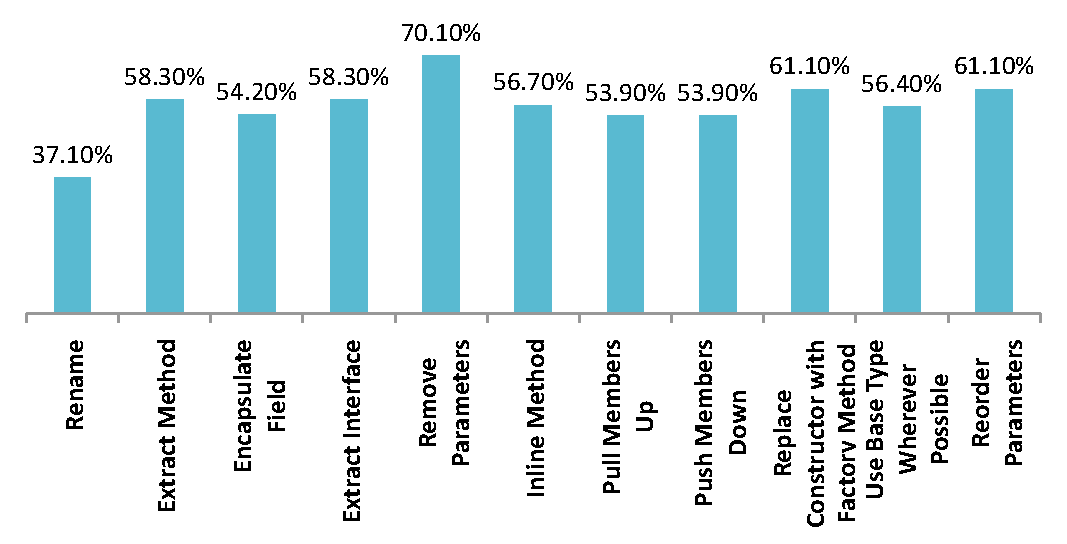
\includegraphics[width=0.55\textwidth]{images/manualRefactoring.pdf}
    \caption{The percentage of survey participants who know individual refactoring types but do those refactorings manually.\cite{Kim2014:EmpiricalStudy}}  
\label{fig:manualRefactoring} 
\end{figure} 

In the same study, when developers are asked {\it ``what percentage of your refactoring is done manually as opposed to using automated refactoring tools?''}, developers answered they do 86\% of refactoring manually on average. Figure~\ref{fig:manualRefactoring} shows the percentages of developers who usually apply individual refactoring types manually despite the awareness of automated refactoring tool support. Vakilian et al.~\cite{Vakilian:2012} and Murphy et al.~\cite{Murphy2006:JSD} also find that programmers do not use automated refactoring despite their awareness of the availability of automated refactorings. Murphy-Hill manually inspected source code produced by 12 developers and found that developers only used refactoring tools for 10\% of refactorings for which tools were available~\cite{Murphy-Hill2012:refactor}. For the question, {\it ``based on your experience, what are the risks involved in refactorings?''}, developers reported regression bugs, code churn, merge conflicts, time taken from other tasks, the difficulty of doing code reviews after refactoring, and the risk of over-engineering. 77\% think that refactoring comes with a risk of introducing subtle bugs and functionality regression~\cite{Kim2012:FSR}.

In a separate study of refactoring tool use, Murphy-Hill et al.~gave developers specific examples of when they did not use refactoring tools, but could have~\cite{Murphy-Hill2012:refactor} and asked why. One reason was that developers started a refactoring manually, but only partway through realized that the change was a refactoring that the IDE offered\textemdash by then, it was too late.  Another complaint was that refactoring tools disrupted their workflow, forcing them to use a tool when they wanted to focus on code.  

\subsubsection{Quantitative Assessment of Refactoring Impact.} 
\label{sec:refactoringassessment} 
While several prior research efforts have conceptually advanced the benefit of refactoring through metaphors, few empirical studies assess refactoring impact quantitatively. Sullivan et al.~first linked software modularity with option theories~\cite{Sullivan1998:option}. A module provides an option to substitute it with a better one without symmetric obligations, and investing in refactoring activities can be seen as purchasing \emph{options} for future adaptability, which will produce benefits when changes happen and the module can be replaced easily. Baldwin and Clark~\cite{Baldwin1999:designrule} argued that the modularization of a system can generate tremendous value in an industry, given that this strategy creates valuable options for module improvement. Ward Cunningham drew the comparison between debt and a lack of refactoring: a quick and dirty implementation leaves {\em technical debt} that incur \emph{penalties} in terms of increased maintenance costs~\cite{Cunningham1992:td}. While these projects advanced conceptual understanding of refactoring impact, they do not quantify the benefits of refactoring.  Kim et al.~\cite{Kim2014:EmpiricalStudy} study on how refactoring impacts inter-module dependencies and defects using the quantitative analysis of Windows 7 version history. Their study finds the top 5\% of preferentially refactored modules experience higher reduction in the number of inter-module dependencies and several complexity measures but increase size more than the bottom 95\%. Based on the hypothesis that measuring the impact of refactoring requires multi-dimensional assessment, they investigate the impact of refactoring on various metrics: churn, complexity, organization and people, cohesiveness of ownership, test coverage and defects.     

MacCormack et al.~\cite{MacCormack2006:study} defined modularity metrics and used these metrics to study evolution of Mozilla and Linux. They found that the redesign of Mozilla resulted in an architecture that was significantly more modular than that of its predecessor. Their study monitored design structure changes in terms of modularity metrics without identifying the modules where refactoring changes are made. Kataoka et al.~\cite{Kataoka2002:metric} proposed a refactoring evaluation method that compares software before and after refactoring in terms of coupling metrics. Kolb et al.~\cite{Kolb2006:refactoring} performed a case study on the design and implementation of existing software and found that refactoring improves software with respect to maintainability and reusability. Moser et al.~\cite{Moser2006:refactoring} conducted a case study in an industrial, agile environment and found that refactoring enhances quality and reusability related metrics. Similarly, Tahvildari et al.~suggested using a catalogue of object-oriented metrics to estimate refactoring impact, including complexity metrics, coupling metrics, and cohesion metrics~\cite{Tahvildari2003:MAE}. 


\subsubsection{Code Smells Detection.} 
\label{sec:codesmell} 

Fowler~\cite{1999:RID} describes the concept of {\em bad smell} as a heuristic for identifying redesign and refactoring opportunities. Example bad smells include code clone and feature envy. Garcia et al.~\cite{Garcia2009:badsmell} proposed several architecture-level bad smells. To automate the identification of bad smells, Moha et al.~\cite{Moha2009:designdefect} presented the Decor tool and domain specific language (DSL) to automate the construction of design defect detection algorithms.  Several other techniques~\cite{Tsantalis2009:extractmethod,Tsantalis2009:movemethod,Tsantalis2008:jdeodorant} automatically identify bad smells that indicate needs of refactorings. For example, Tsantalis and Chatzigeorgiou's technique~\cite{Tsantalis2009:extractmethod} identifies {\em extract method} refactoring opportunities using static slicing. Detection of some specific bad smells such as code duplication has also been extensively researched. Higo et al.~\cite{Higo2004} proposed the Aries tool to identify possible refactoring candidates based on the number of assigned variables, the number of referred variables, and dispersion in the class hierarchy. A refactoring can be suggested if the metrics for the clones satisfy certain predefined values. Koni-N'Sapu~\cite{koni_nsapu:ms01} provides refactoring suggestions based on the location of clones with respect to a system's class hierarchy. Balazinska et al.~\cite{Balazinska2000:ACA} suggest clone refactoring opportunities based on the differences between the cloned methods and the context of attributes, methods, and classes containing clones. Kataoka et al.~used Daikon to infer program invariants at runtime, and suggested candidate refactorings~\cite{Kataoka2001:ASP} using inferred invariants. For instance, if Daikon observes that one parameter of a method is always constant, it then suggests a \emph{removeParameter} refactoring. 
{\it Breakaway} \cite{Cottrell:2007} automatically identifies detailed structural correspondences between two abstract syntax trees to help programmers generalize two pieces of similar code.

Gueheneuc et al.~detect inter-class design defects~\cite{Gueheneuc2001:designdefect} and Marinescu identifies design flaws using software metrics~\cite{Marinescu2004:designflaw}. Izurieta and Bieman detect accumulation of non design-pattern related code~\cite{Izurieta2007:grime}. Guo et al.~define domain-specific code smells~\cite{Guo2010:smell} and investigate the consequence of technical debt~\cite{Guo2011:td}. Tsantalis et al.~ranked clones that have been repetitively or simultaneously changed in the past to suggest refactorings~\cite{Tsantalis2011:rankRefactoring}. Wang et al.~extracted features from code to reflect program context, code smell, and evolution history, and then used a machine learning technique to rank clones for refactorings~\cite{Wang2014:recommendClones}.

Clio~\cite{Wong2011:cleo} detects modularity violations based on the assumptions that multiple types of bad smells are instances of modularity violations that can be uniformly detected by reasoning about modularity hierarchy in conjunction with change locations.  They define {\em modularity violations} as recurring discrepancies between which modules should change together and which modules actually change together according to version histories. For example, when code clones change frequently together, Clio will detect this problem because the co-change pattern deviate from the designed modular structure. Second, by taking version histories as input, Clio detects violations that happened most recently and frequently, instead of bad smells detected in a single version without regard to the program's evolution context. Ratzinger et al.~\cite{ratzinger:msr05} also detect bad smells by examining change couplings but their approach leaves it to developers to identify design violations from visualization of change coupling. 

%Related to the problem of code smells detection, various approaches have been proposed to automatically suggest refactoring opportunities based on program context or version history~\cite{Balazinska2000:ACA,Kataoka2001:ASP,Higo2008:metricrefactoring,Tsantalis2011:rankRefactoring,Wang2014:recommendClones,Meng2015:ARO}. Specifically,
%Balazinska et al.~used a clone detection tool to identify duplicated code and to suggest clone removal refactorings~\cite{Balazinska2000:ACA}. 

\todo{Na: Could you add one or two lines about recent work by Max Di Penta and Denys Poshyvanyk on code smell detection?} 
 

\subsection{Automatic Change Application}
\label{sec:automatic}

\begin{figure}[ht]
 \centering
 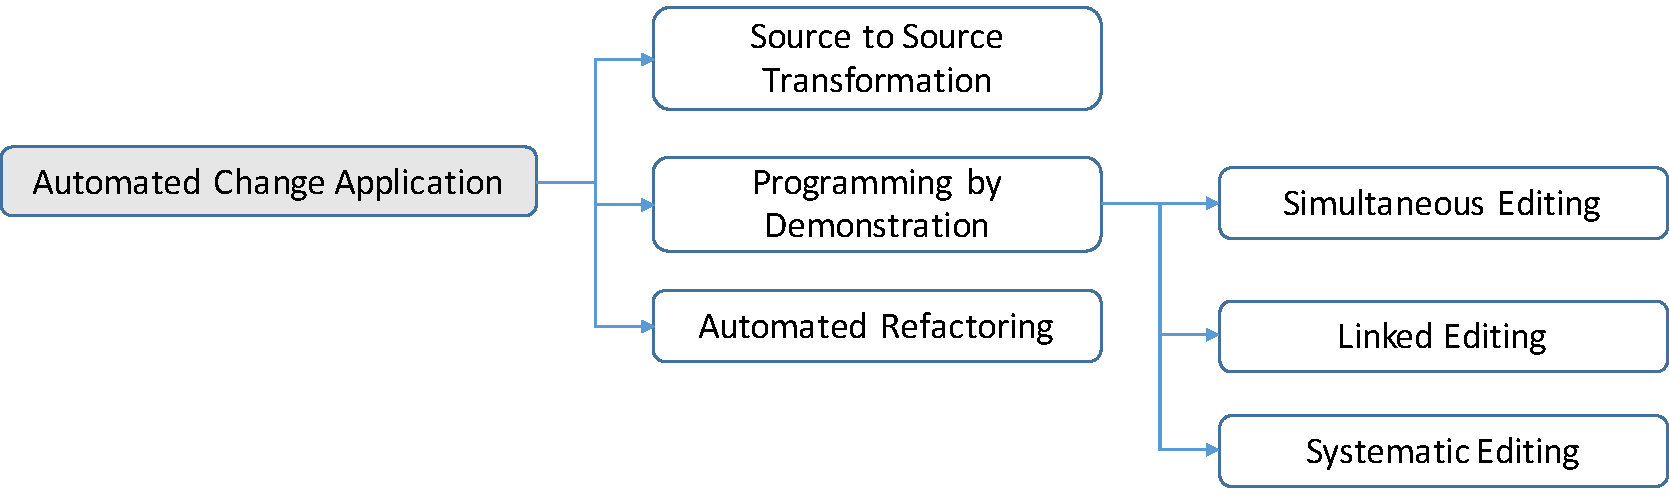
\includegraphics[width=0.95\textwidth]{images/AutomatedChange.pdf}
 \caption{Automated Change Application and Related Research Topics} 
 \label{fig:automaticapplication} 
\end{figure}


Regardless of change types, various approaches are proposed to automatically suggest program changes or reduce the manual effort of updating software. In this section, we discuss automated change application techniques including source-to-source program transformation, Programming by Demonstration (PbD), simultaneous editing, and systematic editing.

\subsubsection{Source Transformation and Languages and Tools.} 

Source transformation tools allow programmers to author their change intent in a formal syntax and automatically update a program using the change script. Most source transformation tools automate repetitive and error-prone program updates. The most ubiquitous and the least sophisticated approach to program transformation is text substitution. More sophisticated systems use program structure information. For example, A* \cite{Ladd1995} and TAWK \cite{Griswold1996} expose syntax trees and primitive data structures. Stratego/XT is based on algebraic data types and term pattern matching\cite{Visser2004}. These tools are difficult to use as they require programmers to understand low-level program representations. TXL attempts to hide these low-level details by using an extended syntax of the underlying programming language~\cite{Cordy2006}. Boshernitsan et al.'s iXJ enables programmers to perform systematic code transformations easily by providing a visual language and a tool for describing and prototyping source transformations. Their user study shows that iXj's visual language is aligned with programmers' mental model of code changing tasks~\cite{Boshernitsan2007}. Coccinelle \cite{Padioleau2008:auto} allows programmers to safely apply crosscutting updates to Linux device drivers. We describe two seminal approaches with more details. 
%Erwig and Ren \cite{Erwig2002} designed a rule-based language to express systematic updates in Haskell. 

\paragraph{\textbf{Example: TXL}} TXL is a programming language and rapid prototyping system specifically designed to support structural source transformation. TXL's source transformation paradigm consists of parsing the input text into a structure tree, transforming the tree to create a new structure tree, and unparsing the new tree to a new output text. Source text structures to be transformed are described using an unrestricted ambiguous context free grammar in extended Backus-Nauer (BNF) form. Source transformations are described by example, using a set of context sensitive structural transformation rules from which an application strategy is automatically inferred. 

Each transformation rule specifies a {\em target type} to be transformed, a {\em pattern} (an example of the particular instance of the type that we are interested in replacing), and a {\em replacement} (an example of the result we want when we find such an instance). In particular, the pattern is an actual source text example expressed in terms of tokens (terminal symbols) and variables (non-terminal types). When the pattern is matched, variable names are bound to the corresponding instances of their types in the match. Transformation rules can be composed like function compositions.  

%As shown in Figure~\ref{fig:txl}, a typical TXL file consists of two parts. The first part defines a context-free grammar to describe program syntax, while the second part describes a set of transformation rules to manipulate the syntax. For our illustrative example, the grammar defines a simple language that only allows numbers, addition and subtraction numerical expressions. The rule \codefont{resolveAddition} describes the resolution of an addition expression by replacing the expression with a number value \codefont{N1 [ + N2 ]}. Given such a file, the TXL program transformation engine automatically transforms programs of the syntactic structure by applying the rules. TXL was used to automate various code translation tasks, like ASP-to-NSP and Java-to-C\#~\cite{Chu:08,Hassan:2005,El-Ramly:2006,Tonella:04}.

TXL programs normally consist of three parts, a context-free “base” grammar for the language to be manipulated, a set of context-free grammatical “overrides” (extensions or changes) to the base grammar, and a rooted set of source transformation rules to implement transformation of the extensions to the base language, as shown in Figure~\ref{fig:txl}. This TXL program overrides the grammar of statements to allow a new statement form. The transformation rule {\tt main} transforms the new form of a statement {\tt V+=E} to an old statement { \tt V:= V+(E)}. In other words, if there are two statements {\tt foo+=bar} and {\tt baz+=boo} they will be transformed to {\tt foo:= foo+(bar)} and {\tt baz:=baz+(boo)} at the source code level. 

\begin{figure}
\centering
\scalebox{0.9}{
	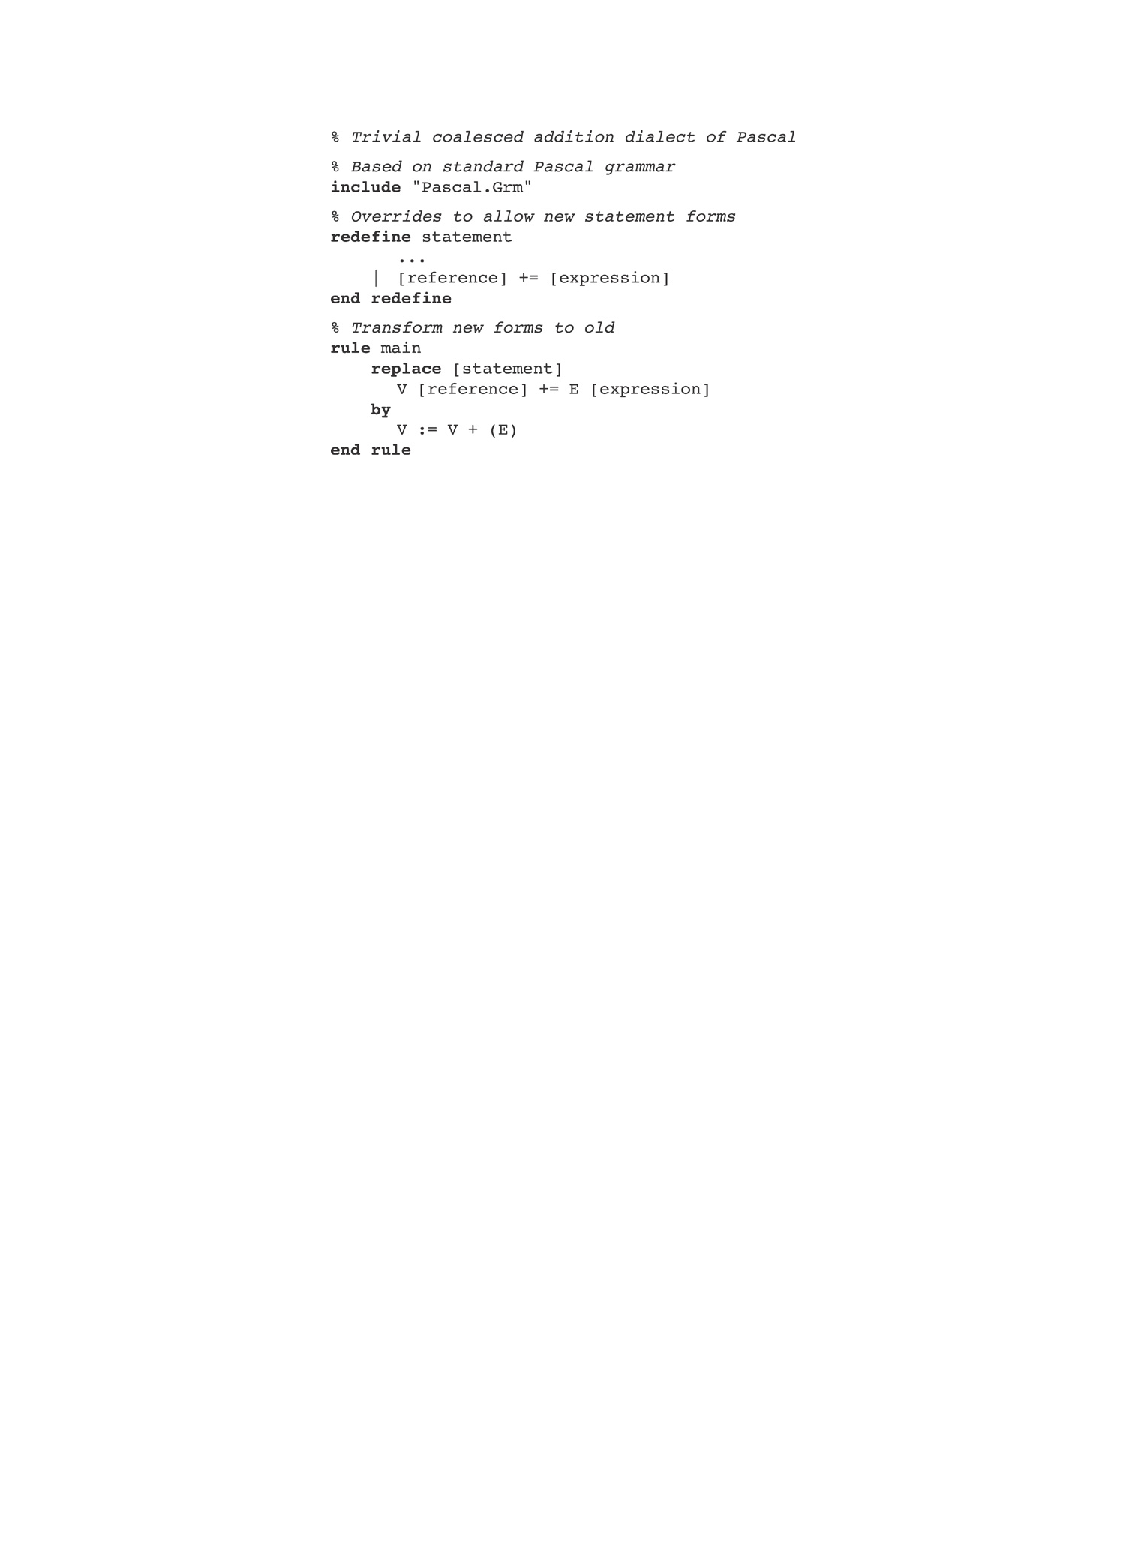
\includegraphics{images/txl2.pdf}
}
\caption{A simple exemplar TXL file based on~\cite{txltour}}
\label{fig:txl}
\end{figure}

\paragraph{\textbf{Example: iXj.}} 
iXj's pattern language consists of a {\em selection pattern} and a {\em transformation action}. A selection pattern is similar to our rules' antecedent, and a transformation action is similar to our rules' consequent. iXj's transformation language allows grouping of code elements using a wild-card symbol \codefont{*}. Figure \ref{ixj_example} shows an example selection pattern and a transformation pattern. 

\begin{figure} 
{\it Selection pattern}: \\
\codefont{* expression instance of java.util.Vector (:obj).removeElement(:method)(* expressions(:args))} \\
\it{Match calls to the {removeElement()} method where the {obj} expression is a subtype of {java.util.Vector}.} \\
{\it Transformation action}:\\
\codefont{\$obj\$.remove(\$obj\$.indexOf(\$args\$))} \\
\it{Replace these calls with with calls to the {remove()} method whose argument is the index of an element to remove.} 
\caption{Example iXj transformation} 
\label{ixj_example} 
\end{figure} 


To reduce the burden of learning the iXj pattern language syntax, iXj's visual editor scaffolds this process through from-example construction and iterative refinement; When a programmer selects an example code fragment to change, iXj automatically generates an initial pattern from the code selection and visualizes all code fragments matched by the initial pattern. The initial pattern is presented in a pattern editor, and a programmer can modify it interactively and see the corresponding matches in the editor. A programmer may edit the transformation action and see the preview of program updates interactively. 

\subsubsection{Programming by Demonstration.} 
Programming by Demonstration is also called Programming by Example (PbE). It is an end-user development technique for teaching a computer or a robot new behaviors by demonstrating the task to transfer directly instead of manually programming the task.  Approaches were built to generate programs based on the text-editing actions demonstrated or text change examples provided by users~\cite{Nix1984,wiki:bsd-comparison,LaH1995,LWD2001}. For instance, TELS records editing actions such as search-and-replace, and generalizes them into a program that transforms input to output~\cite{wiki:bsd-comparison}. It leverages heuristics to match actions against each other to detect any loop in the user-demonstrated program. 

SMARTedit is a representative early effort of applying PbD to text editing. It automates repetitive text-editing tasks by learning programs to perform them using techniques drawn from machine learning~\cite{LWD2001}. SMARTedit represents a text-editing program as a series of functions that alter the state of the text editor (i.e., the contents of the file, or the cursor position). Like macro recording systems, SMARTedit learns the program by observing a user performing her task. However, unlike macro recorders, SMARTedit examines the context in which the user's actions are performed and learns programs that work correctly in new contexts. Below, we describe two seminal PBD approaches applied to software engineering to automate repetitive program changes. 

\paragraph{Simultaneous Editing.}
Simultaneous editing repetitively applies source code changes that are interactively demonstrated by users~\cite{MiM2001}. When users apply their edits in one program context, the tool replicates the \emph{exact lexical} edits to other code fragments, or transforms code accordingly. Linked Editing requires users to first specify the similar code snippets which they want to modify in the same way~\cite{TBG2004}. As users interactively edit one of these snippets, Linked Editing simultaneously applies the identical edits to other snippets. 
%CloneTracker takes the output of a clone detector as input and creates a descriptor for each clone~\cite{DuR2007}. With such descriptors, CloneTracker tracks clones across program versions and identifies any modification to those clones. %Similar to Linked Editing, CloneTracker also echoes edits in one clone to other counterparts upon a developer's request. Clever is another clone management system that tracks code clone groups and detects any inconsistent change applied to clones within the same group~\cite{NNP2009}. If a clone misses the updates applied to the other clones in the same group, Clever automatically suggests the missing update to that clone.

\paragraph{Systematic Editing.} 
Systematic editing is the process of applying similar, but not necessarily identical, program changes to multiple code locations. High-level changes are often systematic\textemdash consisting of related transformations at a code level. Several approaches have been proposed to infer the general program transformation from one or more code change examples provided by developers~\cite{MKM2011,Meng12:lase,Rolim:2017}, and apply the transformation to other program contexts in need of similar changes. Specifically, LASE requires developers to provide multiple similarly changed code examples in Java (at least two)~\cite{Meng12:lase}. By extracting the commonality between demonstrated changes and abstracting the changes in terms of identifier usage and control- or data-dependency constraints in edit contexts, LASE creates a general program transformation, which can both detect code locations that should be changed similarly, and suggest customized code changes for each candidate location. For example, in Figure~\ref{fig:lase}, LASE can take the change example on from $A_{old}$ to $A_{new}$ the code on $B_{old}$ to generate $B_{new}$. Such change is similar but customized to the code on the right. 

\begin{figure}
\centering
\scalebox{0.4}{
	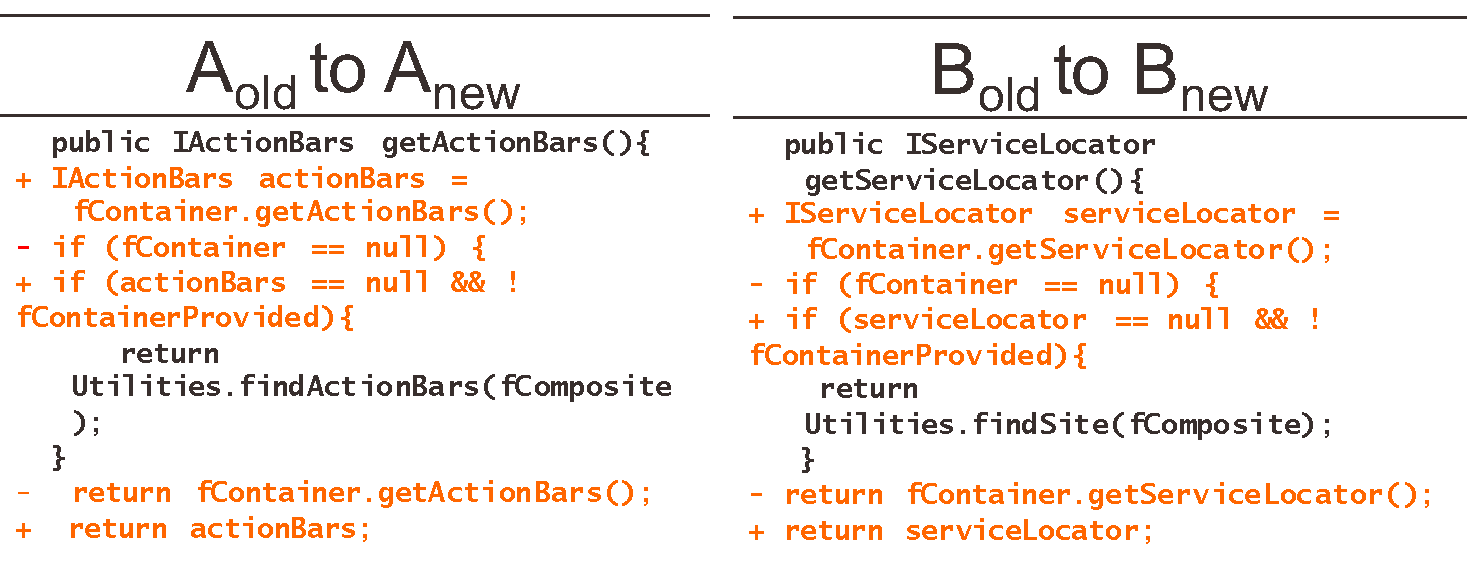
\includegraphics{images/laseexample.pdf}
}
\caption{An example of non-contiguous, abstract edits that can be applied using LASE~\cite{Meng12:lase}}
\label{fig:lase}
\end{figure}


 

%\subsection{Other Studies of Software Evolution and its Visualization} 
%\input{evolutionvis} 

\section{An Organized Tour of Seminal Papers: II. Inspecting Changes}

Section~\ref{sec:codereview} presents the brief history of software inspection and discuss emerging themes from modern code review practices. Subsections from~\ref{sec:reviewtool} to~\ref{sec:inconsistent} discuss various methods that help developers better comprehend software changes, including {\em change decomposition}, {\em refactoring reconstruction}, {\em conflict} and {\em interference} detection, {\em related change search}, and {\em inconsistent change detection}. Section~\ref{sec:differencing} describes various program differencing techniques that serve as a basis for analyzing software changes. Section~\ref{sec:record} describes complementary techniques that record software changes during programming sessions. 

\begin{figure}[ht]
 \centering
 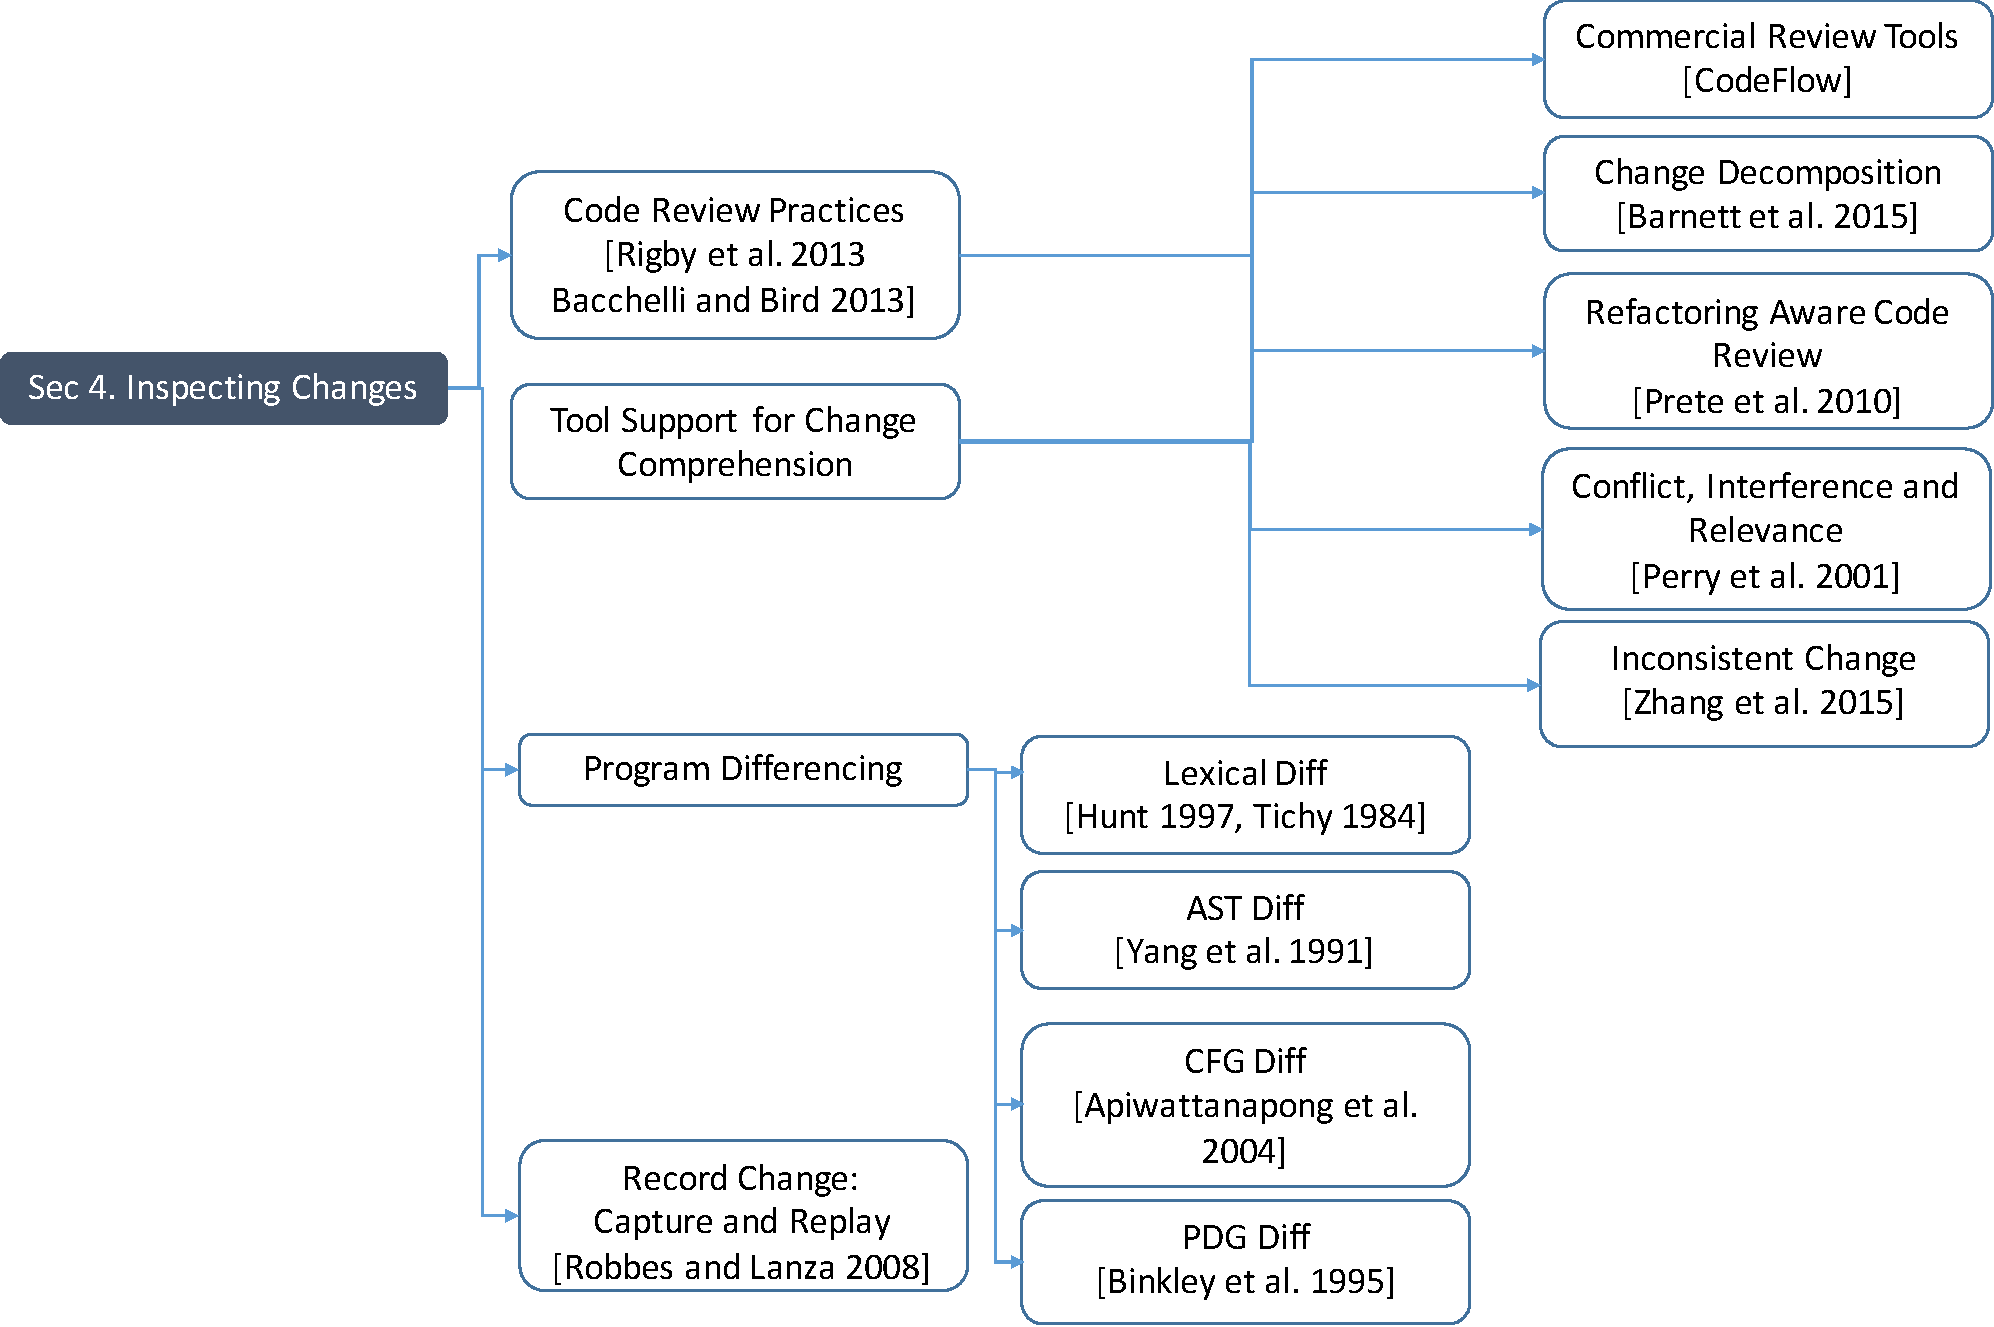
\includegraphics[width=0.95\textwidth]{images/ChangeInspection.pdf}
 \caption{Change Inspection and Related Research Topics} 
 \label{fig:changeinspection} 
\end{figure}

\subsection{Software Inspection and Modern Code Review Practices} 
\label{sec:codereview}

To improve software quality during software evolution, developers often perform {\em code reviews} to manually examine software changes. Michael Fagan from IBM first introduced ``code inspections'', in a seminal paper in 1976~\cite{Fagan1999:checklist}. Code inspections are performed at the end of major software development phases, with the aim of finding overlooked defects before moving to the next phase. Software artifacts are circulated a few days in advance and then reviewed and discussed in a series of meetings. The review meetings include the author of an artifact, other developers to assess the artifact, and a meeting chair to moderate the discussion, and a secretary to record the discussion. Over the years, code inspections have been proven a valuable method to improve software quality. However, the cumbersome and time-consuming nature of this process hinders its universal adoption in practice~\cite{johnson1998reengineering}. 

\begin{figure}[ht]
 \centering
 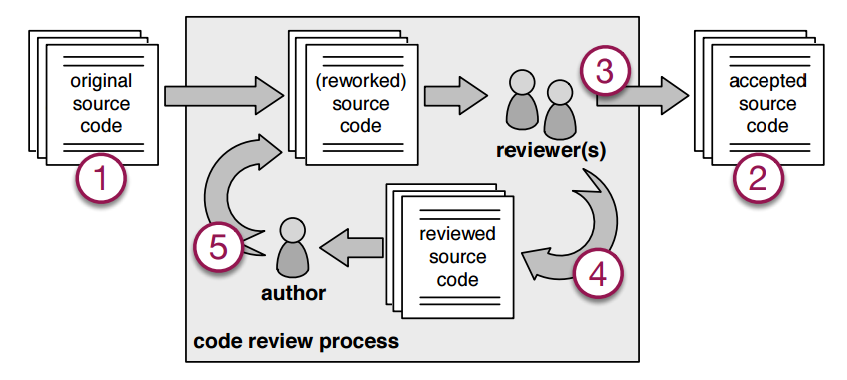
\includegraphics[width=0.75\textwidth]{images/review-process.png}
 \caption{Modern Code Review Process~\cite{beller2014modern}}
 \label{fig:review-process}
\end{figure}

To avoid the inefficiencies in code inspections, most open-source and industrial projects adopt a lightweight, flexible code review process, which we refer to as {\em modern code reviews}. Figure~\ref{fig:review-process} shows the workflow of modern code reviews. The {\em author} first submits the {\em original source code} for review. The {\em reviewers} then decide whether the submitted code meets the quality acceptance criteria. If not, reviewers can annotate the source code with review comments and send back the {\em reviewed source code}. The author then revises the code to address reviewers' comments and send it back for further reviews. This process continues till all reviewers accept the revised code.

In contrast to formal code inspections (Fagan style), modern code reviews occur more regularly and informally on program changes. Rigby et al.~conducted the first case study about modern code review practices in an open-source software (OSS), Apache HTTP server, using archived code review records in email discussions and version control histories~\cite{Rigby2008:apache}. They described modern code reviews as ``early, frequent reviews of small, independent, complete contributions conducted asynchronously by a potentially large, but actually small, group of self-selected experts.'' As code reviews are practiced in software projects with different settings, cultures, and policies, Rigby and Bird further investigated code review practices using a diverse set of open-source and industrial projects~\cite{rigby2013convergent}. Despite differences among projects, they found that many characteristics of modern code reviews have converged to similar values, indicating general principles of modern code review practices. We summarize these convergent code review practices as following.

\begin{itemize}
\item {\it Modern code reviews occur early, quickly, and frequently.} Traditional code inspections happen after finishing a major software component and often last for several weeks. In contrast, modern code reviews happen more frequently and quickly when software changes are committed. For example, the Apache project has review intervals between a few hours to a day. Most reviews are picked up within a few hours among all projects, indicating that reviewers are regularly watching and performing code reviews~\cite{rigby2013convergent}.

\item {\it Modern code reviews often examine small program changes.} During code reviews, the median size of software change varies from 11 to 32 changed lines. The change size is larger in industrial projects, e.g, 44 lines in Android, 78 lines in Chrome, but still much smaller than code inspections, e.g., 263 lines in Lucent. Such small changes facilitate developers to constantly review changes and thus keep up-to-date with the activities of their peers. 
\item {\it Modern code reviews are conducted by a small group of self-selected reviewers.} In OSS projects, no reviews are assigned and developers can select the changes of interest to review. Program changes and review discussions are broadcast to a large group of stakeholders but only a small number of developers periodically participate in code reviews. In industrial projects, reviews are assigned in a mixed manner---the author adds a group of reviewer candidates and individuals from the group then select changes based on their interest and expertise. On average, two reviewers find an optimal number of defects~\cite{rigby2013convergent}.

\item {\it Modern code reviews are often tool-based.} There is a clear trend towards utilizing review tools to support review tasks and communication. Back in 2008, code reviews in OSS projects were often email-based due to a lack of tool support~\cite{Rigby2008:apache}. In 2013 study, some OSS projects and all industrial projects they studied used a review tool~\cite{rigby2013convergent}. More recently, popular OSS hosting services such as GitHub and BitBucket have integrated lightweight review tools to assign reviewers, enter comments, and record discussions. Compared with email-based reviews and traditional software inspections, tool-based reviews provide the benefits of traceability. 

\item {\it Although the initial purpose of code review is to find defects, recent studies find that the practices and actual outcomes are less about finding defects than expected.} A study of code reviews at Microsoft found that only a small portion of review comments were related to defects, which were mainly about small, low-level logical issues~\cite{bacchelli2013expectations}. Rather, code review provides a spectrum of benefits to software teams, such as knowledge transfer, team awareness, and improved solutions with better practices and readability. 

\end{itemize} 

\subsubsection{Commercial Code Review Tools.} 
\label{sec:reviewtool} 

There is a proliferation of review tools, e.g., Phabricator,\footnote{\url{http://phabricator.org}} Gerrit,\footnote{\url{http://code.google.com/p/gerrit/}} CodeFlow,\footnote{\url{http://visualstudioextensions.vlasovstudio.com/2012/01/06/codeflow-code-review-tool-for-visual-studio/}} Crucible,\footnote{\url{https://www.atlassian.com/software/crucible}} and Review Board.\footnote{\url{https://www.reviewboard.org/}} We illustrate CodeFlow, a collaborative code review tool at Microsoft. Other review tools share similar functionality as CodeFlow.

\begin{figure}[ht]
 \centering
 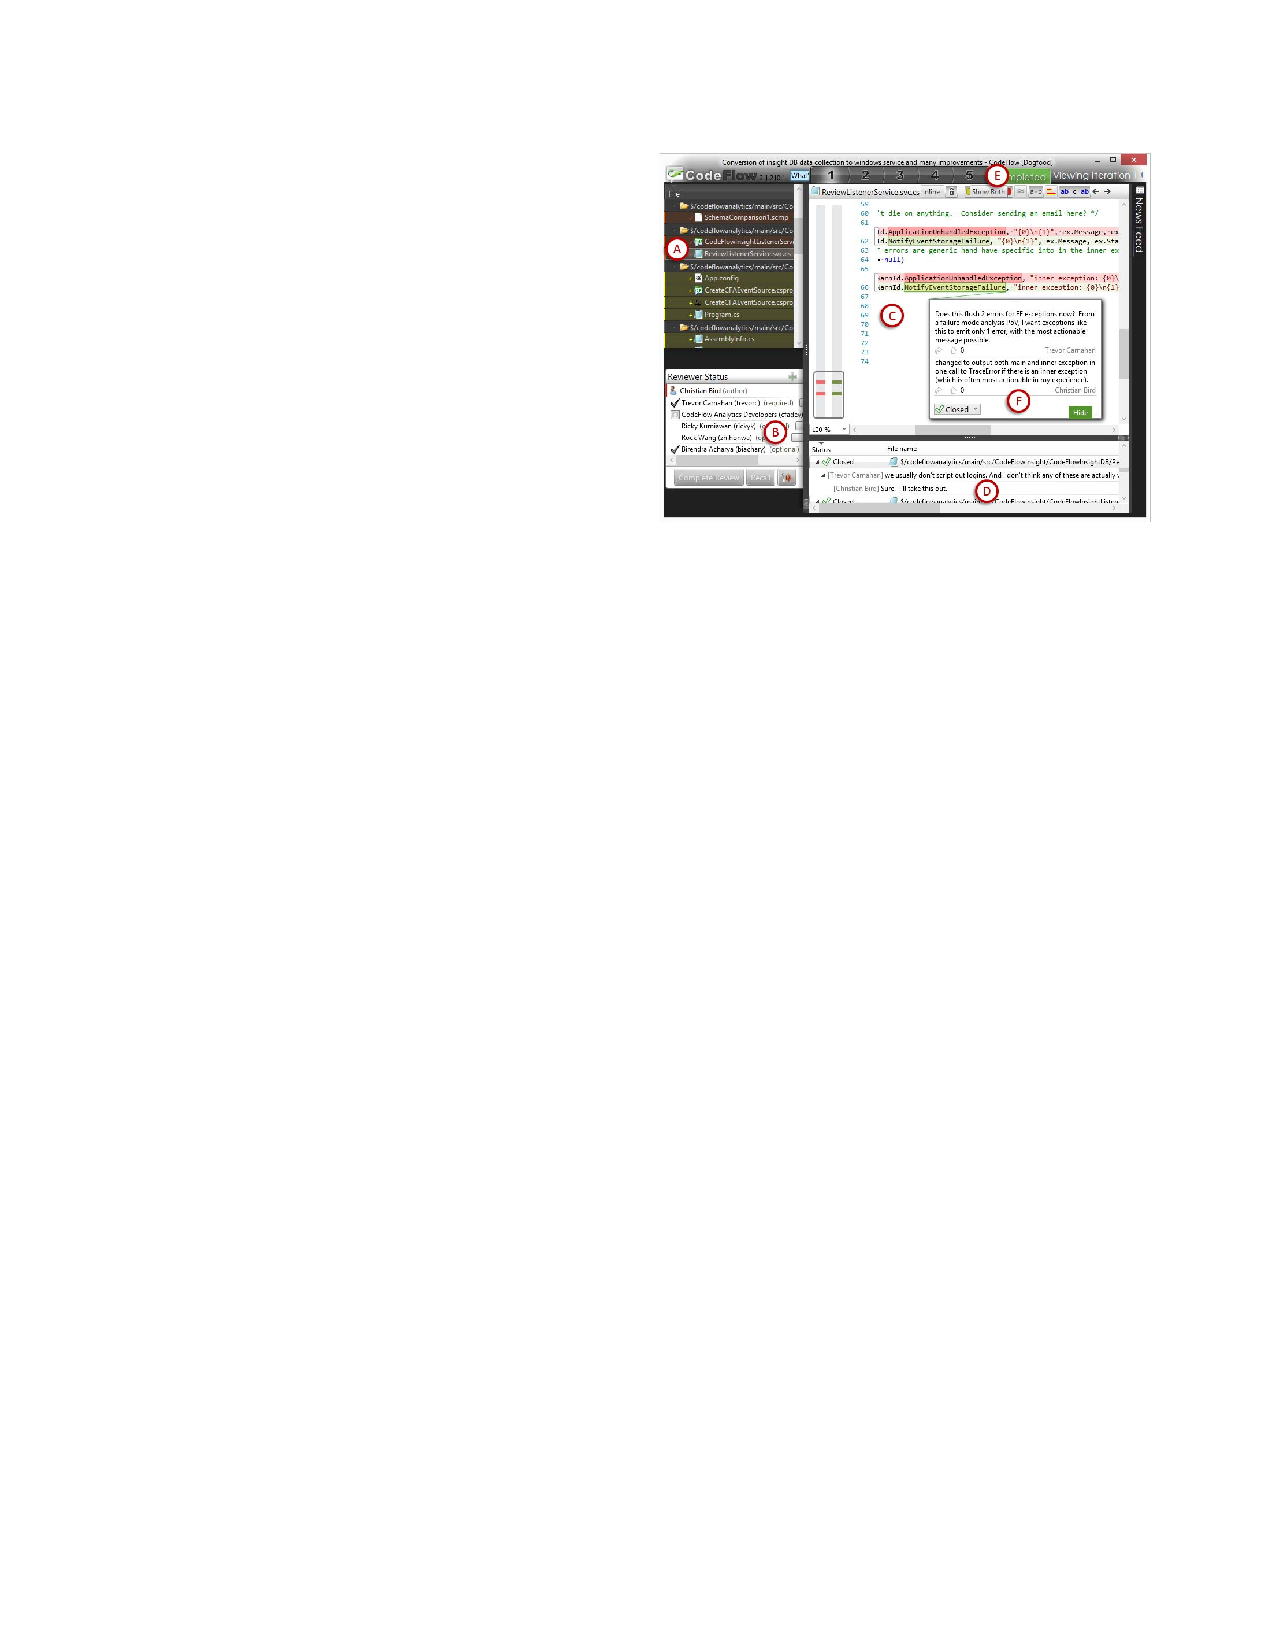
\includegraphics[width=0.75\textwidth]{images/codeflow.pdf}
 \caption{Example of Code Review using CodeFlow~\cite{bosu2015characteristics}}
 \label{fig:codeflow}
\end{figure}

To create a review task, a developer uploads changed files with a short description to CodeFlow. Reviewers are then notified via email and they can examine the software change in CodeFlow. Figure~\ref{fig:codeflow} shows the desktop window of CodeFlow. It includes a list of changed files under review (A), the reviewers and their status (B), the highlighted diff in a changed file (C), a summary of all review comments and their status (D), and the iterations of a review (E). If a reviewer would like to provide feedback, she can select a change and enter a comment which is overlayed with the selected change (F). The author and other reviewers can follow up the discussion by entering comments in the same thread. Typically, after receiving feedback, the author may revise the change accordingly and submit the updated change for additional feedback, which constitutes another review cycle and is termed as an {\em iteration}. In Figure~\ref{fig:codeflow}-E, there are five iterations. CodeFlow assigns a status label to each review comment to keep track of the progress. The initial status is ``Active'' and can be changed to ``Pending'', ``Resolved'', ``Won't Fix'', and ``Closed'' by anyone. Once a reviewer is satisfied with the updated changes, she can indicate this by setting their status to ``Signed Off''. After enough reviewers signed off\textemdash sign-off policies vary by team\textemdash the author can commit the changes to the source repository.

Commercial code review tools facilitate management of code reviews but do not provide deep support for change comprehension. According to Bachhelli et al.~\cite{bacchelli2013expectations}, understanding program changes and their contexts remains a key challenge in modern code review. Many interviewees acknowledged that it is difficult to understand the rationale behind specific changes. All commercial review tools show the highlighted {\em textual, line-level diff} of a changed file. However, when the code changes is distributed across multiple files, developers find it difficult to inspect code changes~\cite{Dunsmore2000:ooinspection}. This obliges reviewers to read changed lines file by file, even when those cross-file changes are done systematically to address the same issue. 
\subsubsection{Change Decomposition.}
\label{sec:decomposition} 

Prior studies also observe that developers often package program changes of multiple tasks to a single code review~\cite{Kawrykow2011,Murphy-Hill2012:refactor,herzig2013impact}. Such large, unrelated changes often lead to difficulty in inspection, since reviewers have to mentally ``untangle'' them to figure out which subset addresses which issue. Reviewers indicated that they can better understand small, cohesive changes rather than large, tangled ones~\cite{Rigby2008:apache}. For example, a code reviewer commented on Gson revision 1154 saying ``{\em I would have preferred to have two different commits: one for adding the new {\ttt getFieldNamingPolicy} method, and another for allowing overriding of primitives.}''\footnote{\url{https://code.google.com/p/google-gson/source/detail?r=1154}} Among change decomposition techniques~\cite{tao2015partitioning,barnett2015helping}, we discuss a representative technique called {\clusterchanges}. 

{\clusterchanges} is a lightweight static analysis technique for decomposing large changes~\cite{barnett2015helping}. The insight is that program changes that address the same issue can be related via implicit dependency such as {\em def-use} relationship. For example, if a method definition is changed in one location and its call-sites are changed in two other locations, these three changes are likely to be related and should be reviewed together. Given a code review task, {\clusterchanges} first collects the set of definitions for types, fields, methods, and local variables in the corresponding project under review. Then {\clusterchanges} scans the project for all uses (i.e., references to a definition) of the defined code elements. For instance, any occurrence of a type, field, or method either inside a method or a field initialization is considered to be a use. Based on the extracted def-use information, {\clusterchanges} identifies three relationships between program changes. 

\begin{itemize}
	\item {\bf Def-use relation}. If the definition of a method or a field is changed, all the uses should also be updated. The change in the definition and the corresponding changes in its references are considered related.
	\item {\bf Use-use relation}. If two or more uses of a method or a field defined within the change-set are changed, these changes are considered related. 
	\item  {\bf Enclosing relation}. Program changes in the same method are considered related, under the assumption that  (1) program changes to the same method are often related, and (2) reviewers often inspect methods atomically rather than reviewing different changed regions in the same method separately.
\end{itemize} 

Given these relations, {\clusterchanges} creates a partition over the set of program changes by computing a transitive closure of related changes. On the other hand, if a change is not related to any other changes, it will be put into a specific partition, {\em miscellaneous changes}.


\subsubsection{Refactoring Aware Code Review.}  
\label{sec:refactoringreview} 

Identifying which refactorings happened between two program versions is an important research problem, because inferred refactorings can help developers understand software modifications made by other developers during peer code reviews. Reconstructed refactorings can be used to update client applications that are broken due to refactorings in library components. Furthermore, they can be used to study the effect of refactorings on software quality empirically when the documentation about past refactorings is unavailable in software project histories. 

{\bf Refactoring reconstruction} techniques compare the old and new program versions and identify corresponding entities based on their {name similarity} and {structure similarity}\cite{Demeyer2000, Zou2005, Malpohl2000, Dig2006, Weissgerber2006}. Then based on how basic entities and relations changed from one version to the next, concrete refactoring type and locations are inferred. For example, Xing et al.'s approach~\cite{UMLDiff2005} UMLDiff extracts class models from two versions of a program, traverses the two models, and identifies corresponding entities based on their {name similarity} and {structure similarity} {(i.e., similarity in type declaration and uses, field accesses, and method calls)}. Xing {et al.} later presented an extended approach to refactoring reconstruction based on change-facts {\em queries}~\cite{Eleni01}. They first extract facts regarding design-level entities and relations from each individual source code version. These facts are then pairwise compared to determine how the basic entities and relations have changed from one version to the next. Finally, queries corresponding to well-known refactoring types are applied to the change-facts database to find concrete refactoring instances. Among these refactoring reconstruction techniques, we introduce a representative example of refactoring reconstruction, called RefFinder in details~\cite{Prete2010:reffinder,Kim2010:reffinder}.   

% Demeyer {et al.} first proposed the idea of inferring refactorings from two program versions by comparing two program versions. They used a set of ten characteristic metrics, such as LOC and the number of method calls within a method~\cite{Demeyer2000}. Zou and Godfrey first coined the term origin analysis, which serves as a basis for refactoring reconstruction by matching code elements using multiple criteria (e.g., names, signatures, metric values, callers, and callees)~\cite{Zou2005}. Their approach infers merge, split, and rename refactorings. Van Rysselberghe and Demeyer used a clone detector to detect moved methods~\cite{Rysselberghe2003}.  Antoniol {et al.} identified class-level refactorings using a vector space information retrieval approach~\cite{Antoniol2004}. Malpohl {et al.} \cite{Malpohl2000} align tokens using {\it diff} and infers a function or variable renaming when distinct tokens are surrounded by mapped token pairs. Dig et al.'s approach, {Refactoring Crawler} identifies refactorings in two stages~\cite{Dig2006}. First, it finds a list of code element pairs using {\em shingles} (a metric-based fingerprint) and performs a semantic analysis based on reference relationships (calls, instantiations, uses of types, import statements). The second part of the algorithm is an iterative, fix point algorithm that considers refactorings in a top-down order. 

%Wei{\ss}gerber and Diehl's approach~\cite{Weissgerber2006} extracts added and deleted entities (fields, methods, and classes) by parsing deltas from a version control system and then compares these entities based on their {name similarity}. When it cannot disambiguate all refactoring candidates, it uses a {clone detector} (CCFinder~\cite{Kamiya2002}) to rank these candidates. S. Kim et al.'s approach~\cite{SKim2005} considers various information (such as {calling relationships}, {clone detection} results, and {name similarity}) to match method-headers.  Wu et al.'s approach~\cite{Wu2010:AHA} is a hybrid approach that combines the strengths of {call-graph matching} and {name-similarity} based matching. Nguyen et al.'s approach~\cite{Nguyen2010:GAA} identifies refactorings in libraries to support adaptation of the client applications that use those libraries. Similar to Xing et al.'s approach, the algorithm matches code elements top-down based on method name similarity and method body contents. Fluri et al.'s approach~\cite{FWP2007} compares two versions of abstract syntax trees, computes tree-edit operations, and maps each tree-edit to atomic AST-level change types (e.g., parameter ordering change).

\label{sec:intro} 
\begin{figure*}
\centering
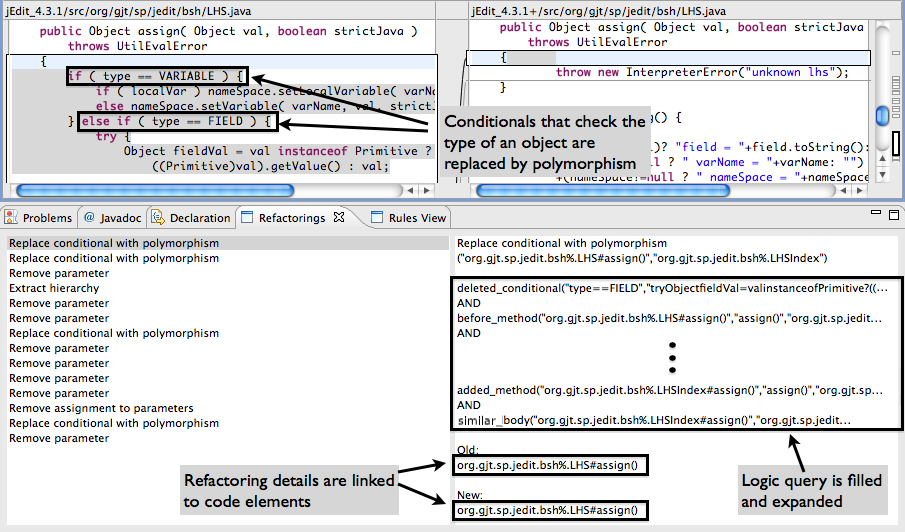
\includegraphics[width=0.95\textwidth]{images/reffinder.png}
\caption{RefFinder infers a {\it replace conditionals with polymorphism} refactoring from change facts {\it deleted\_conditional}, {\it after\_subtype}, {\it before\_method}, {\it added\_method} and {\it similar\_body}.\cite{Kim2010:reffinder}}
 \label{fig:reffinderscreenshot}
\end{figure*}

\paragraph{Example: RefFinder.}

{\em RefFinder} is a logic-query based approach for inferring various types of refactorings in Fowler's catalog~\cite{Prete2010:reffinder}. It first encodes each refactoring type as a structural constraint on the program before and after the refactoring in a template logic rule. It then compares the syntax tree of each version to compute change facts such as {\tt added\-\_subtype}, at the level of code elements (packages, types, methods, and fields), structural dependencies (subtyping, overriding, method-calls, and field-accesses), and control constructs (while, if-statements, and try-catch blocks). It determines a refactoring inference order to find atomic refactorings before composite refactorings. 

For example, consider an \emph{extract superclass} refactoring that extracts common functionality in different classes into a superclass. It finds each {\it pull-up-method} refactoring and then tests if they combine to an \emph{extract superclass} refactoring. For each refactoring rule, it converts the antecedent of the rule to a logic query and invokes the query on the change-fact database. If the query returns the constant bindings for logic variables, it creates a new logic fact for the found refactoring instance and {\em writes} it to the fact-base. For example, by invoking a query {\tt pull\-\_up\_method\-(?method, ?class, ?superclass) $\wedge$ added\_type\-(?superclass)}, it finds a concrete instance of {\it extract superclass} refactoring. Figure~\ref{fig:complexrefactoring} illustrates an example refactoring reconstruction process. 

\begin{figure}
\scriptsize
%\centering 
\begin{tabular}{|p{0.17\textwidth}|p{0.83\textwidth}|}
\hline
{pull\_up\_method} & You have methods with identical results on subclasses; move them to the superclass. \\
\hline
template &
\factfont{deleted\_method(m1, n, t1) $\wedge$ after\_subtype(t2, t1) $\wedge$ added\_method(m1, n, t2) $\Rightarrow$ pull\_up\_method(n, t1, t2)}  \\
\cline{1-2}
logic rules&  \factfont{pull\_up\_method(m1, t1, t2) $\wedge$ added\_type(t2) $\Rightarrow$ extract\_superclass(t1,t2)} \\
\hline
code example & \vspace{-5mm} 
\begin{verbatim} 
+public class Customer{ 
+   chargeFor(start:Date, end:Date) { ... } ...}  
-public class RegularCustomer{
+public class RegularCustomer extends Customer{
-   chargeFor(start:Date, end:Date){ ... } ...}
+public class PreferredCustomer extends Customer{ 
- chargeFor(start:Date, end:Date){ ... } // deleted ... } 
\end{verbatim} 
\vspace{-5mm}
\\ \hline
found &
\factfont{pull\_up\_method("chargeFor", "RegularCustomer", "Customer")} \\

refactorings& \factfont{pull\_up\_method("chargeFor", "PreferredCustomer", "Customer")}  \\
& \factfont{extract\_superclass("RegularCustomer", "Customer")} \\
& \factfont{extract\_superclass("PreferredCustomer", "Customer")}\\
\hline
\end{tabular}
\caption{Reconstruction of \emph{Extract Superclass} Refactoring} 
\label{fig:complexrefactoring}
\end{figure} 

This approach has two advantages over other approaches. First, it analyzes the body of methods including changes to the control structure within method bodies. Thus, it can handle the detection of refactorings such as {\it replacing conditional code with polymorphism}. Second, it handles composite refactorings, since the approach reasons about which constituent refactorings must be detected first and reason about how those constituent refactorigs are knit together to detect higher-level, composite refactorings. It supports 63 out of 72 refactoring types in Fowler's catalog. As shown in Figure \ref{fig:reffinderscreenshot}, RefFinder visualizes the reconstructed refactorings as a list.  The panel on the right summarizes key details of the selected refactoring and allows the developer quickly navigate to the associated code fragments. 

\subsubsection{Change Conflicts, Interference, and Relevance. } 
\label{sec:conflict} 
As development teams become distributed, and the size of the system is often too large to be handled by a few developers, multiple developers often work on the same module at the same time. In addition, the market-pressure to develop new features or products makes parallel development no longer an option.  A study on a subsystem of Lucent 5ESS telephone found that 12.5\% of all changes are made by different developers to the same files within 24 hours, showing a high degree of parallel updates~\cite{Perry2001:parallel}. A subsequent study found that even though only 3\% of the changes made within 24 hours by different developers physically overlapped each other's changes at a textual level but there was a high degree of semantic interference among parallel changes at a data flow analysis level (about 43\% of revisions made within one week). They also discovered a significant correlation between files with a high degree of parallel development and the number of defects~\cite{Shao2007:interference}. 

Most version control systems are only able to detect most simple types of conflicting changes\textemdash changes made on top of other changes~\cite{mens:survey02}. To detect changes that indirectly conflict with each other, some define the notion of {\em semantic interference} using program slicing on program dependence graphs, and integrate non-interfering versions only if there is no overlap between program slices~\cite{Horwitz1989}. As another example, some define semantic interference as the overlap between the data-dependence based impact sets of parallel updates~\cite{Shao2007:interference}. 

Several techniques identify related changes across revisions rely on temporal proximity \cite{Bevan2005, Fischer2003, German2004:softchange, Zimmermann2004b}, syntactic dependence \cite{Chesley2005}, physical location \cite{Zeller1999}, committer information \cite{Fischer2003, German2004:softchange, Zimmermann2004b}, history of co-changes \cite{Gall1998, Ying2004, Zimmermann2004}, and content similarity~\cite{Kim:2009,NNP2009}. For example, Crisp \cite{Chesley2005} computes atomic structural changes such as method additions and deletions via AST differencing and groups syntactically dependent changes through def-use relationships.

%\subsubsection{Search of Software Changes.}
%\label{sec:changesearch} 

%SCM query systems such as SCQL \cite{Hindle2005} or CVS Query \cite{bonsai} can search check-ins based on who changed which file and when, but cannot search change history by code elements and dependencies. Systems such as Hipikat \cite{Hipikat}, Bridge \cite{Venolia2006:bridge}, Tesseract \cite{Tesseract}, and Deep Intellisense \cite{Holmes2008:intellisense} automatically associate different types of software artifacts (e.g., check-ins, bug reports, and emails) but provide limited help in querying code changes. 

%Several visualization tools focus on representing changes between versions \cite{Ball1996,Eick2002,Girba2004,Holt1996,Lanza01:sv,Lanza2003,Rysselberghe2004a}. For example, Evolution Matrix \cite{Lanza01:sv} visualizes classes that have been added, modified, and deleted in different versions and creates a 2-D matrix where the rows represent classes and the columns represent the versions of the artifact. These tools generally require substantial interpretation effort by developers to understand system evolution. Studying program evolution by analyzing existing software project artifacts is increasingly becoming a popular research approach. Existing research infrastructures for mining software artifacts focus on data extraction \cite{Bevan2005,Fischer2003} and integration of different types of software artifacts \cite{Hipikat, Venolia2006:bridge,Tesseract, Begel2010:codebook}. 

\subsubsection{Detecting and Preventing Inconsistent Changes to Clones.} 
\label{sec:inconsistent} 

Code cloning is an important source of bugs in operating systems~\cite{releasenote}. In 65\% of the ported code, at least one identifier is renamed, and in 27\% cases at least one statement is inserted, modified, or deleted~\cite{Li2004:CP-Miner}. An incorrect adaptation of ported code often leads to porting errors~\cite{Jiang2007}. Interviews with developers confirm that inconsistencies in clones are indeed bugs and report that {\em ``nearly every second, unintentional inconsistent changes to clones lead to a fault."}~\cite{Juergens2009:clone-bug}.  Several techniques find inconsistent changes to similar code fragments by tracking copy-paste code and by comparing the corresponding code and its surrounding contexts~\cite{Li2004:CP-Miner, Jablonski2007:CReN, Ray2013:spa, Jiang2007, Jiang2007a}.  Below, we present a representative technique, called {\critics}. 
%For example, SPA detects a broader scope of inconsistent renamings by tokenizing function names, file names, and identifier names using a camel case naming convention and mapping corresponding tokens. Our algorithm detects an inconsistency when a token in one context maps to multiple tokens in the other context.  For example, when code is ported from~\texttt{Export.java} to~\texttt{Import.java}, SPA checks whether all names related to~\texttt{export} are updated to~\texttt{import}.  ~\cite{Ray2013:spa} 

% Jiang et al.~show that an inconsistent context can also cause porting errors~\cite{Jiang2007}. However, their definition of context is limited to the {\em innermost} control flow construct surrounding the cloned code. They identify syntactic clones using AST level similarity~\cite{Jiang2007a}, and then detect inconsistencies by comparing the contexts. 
%DejaVu extends the work by Jiang et al. by using several filtering heuristics, such as assessing textual similarity and pruning non-cloned contexts, to improve its precision~\cite{Gabel2010:dejavu}. 

\begin{figure}[ht]
 \centering
 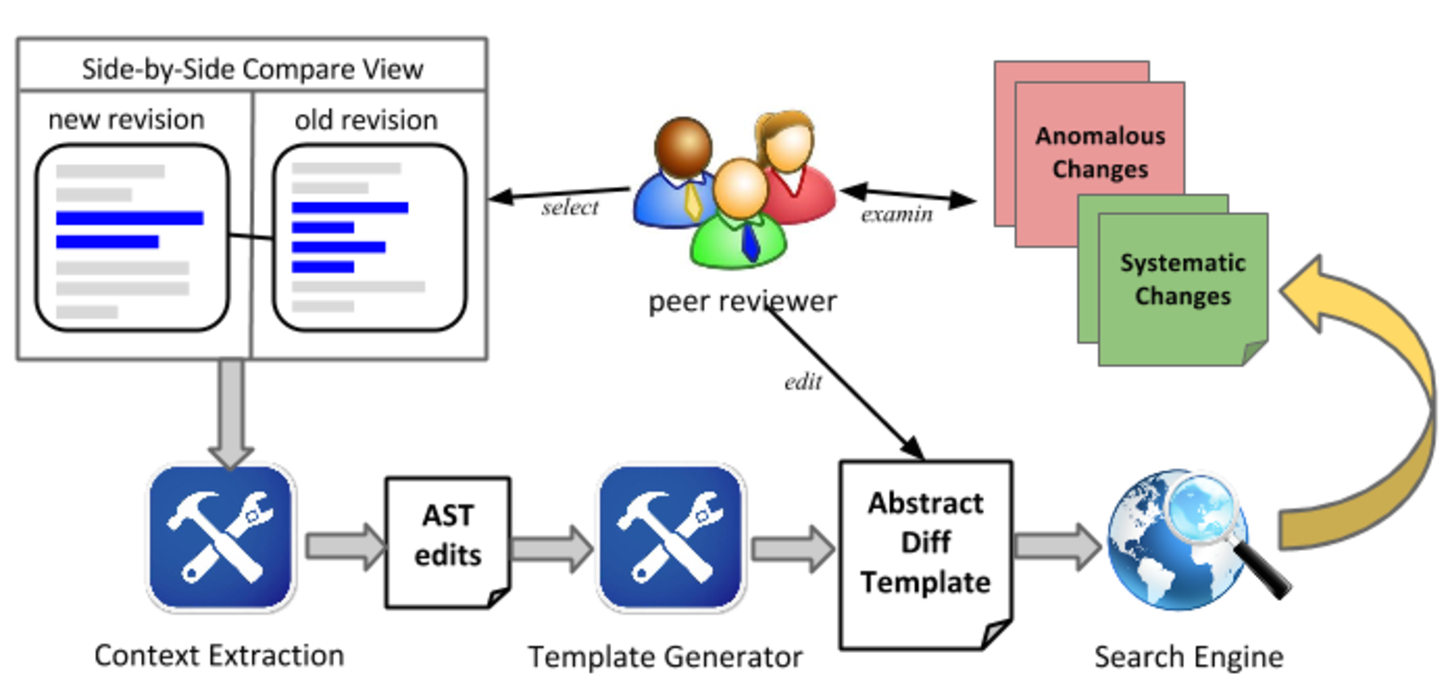
\includegraphics[width=0.8\textwidth]{images/critics-workflow.pdf}
 \caption{The workflow of {\critics}}
 \label{fig:critics-workflow}
\end{figure}

\paragraph{Example: {\critics}.} It allows reviewers to interactively detect inconsistent changes during peer code review~\cite{zhang2015interactive}. 
Given a specified change that a reviewer would like to inspect, {\critics} creates a change template from the selected change, which serves as the pattern for searching similar changes. {\critics} includes {\em change context} in the template---unchanged, surrounding program statements that are relevant to the selected change. {\critics} models the template as Abstract Syntax Tree (AST) edits and allows reviewers to iteratively customize the template by parameterizing its content and by excluding certain statements. {\critics} then matches the customized template against the rest of the codebase to summarize similar changes and locate potential inconsistent or missing changes. Reviewers can incrementally refine the template and progressively search for similar changes until they are satisfied with the inspection results. This interactive feature allows reviewers with little knowledge of a codebase to flexibly explore the program changes with a desired pattern. Figure~\ref{fig:critics-workflow} describes the interactive workflow of {\critics}. 

\begin{figure}[ht]
 \centering
 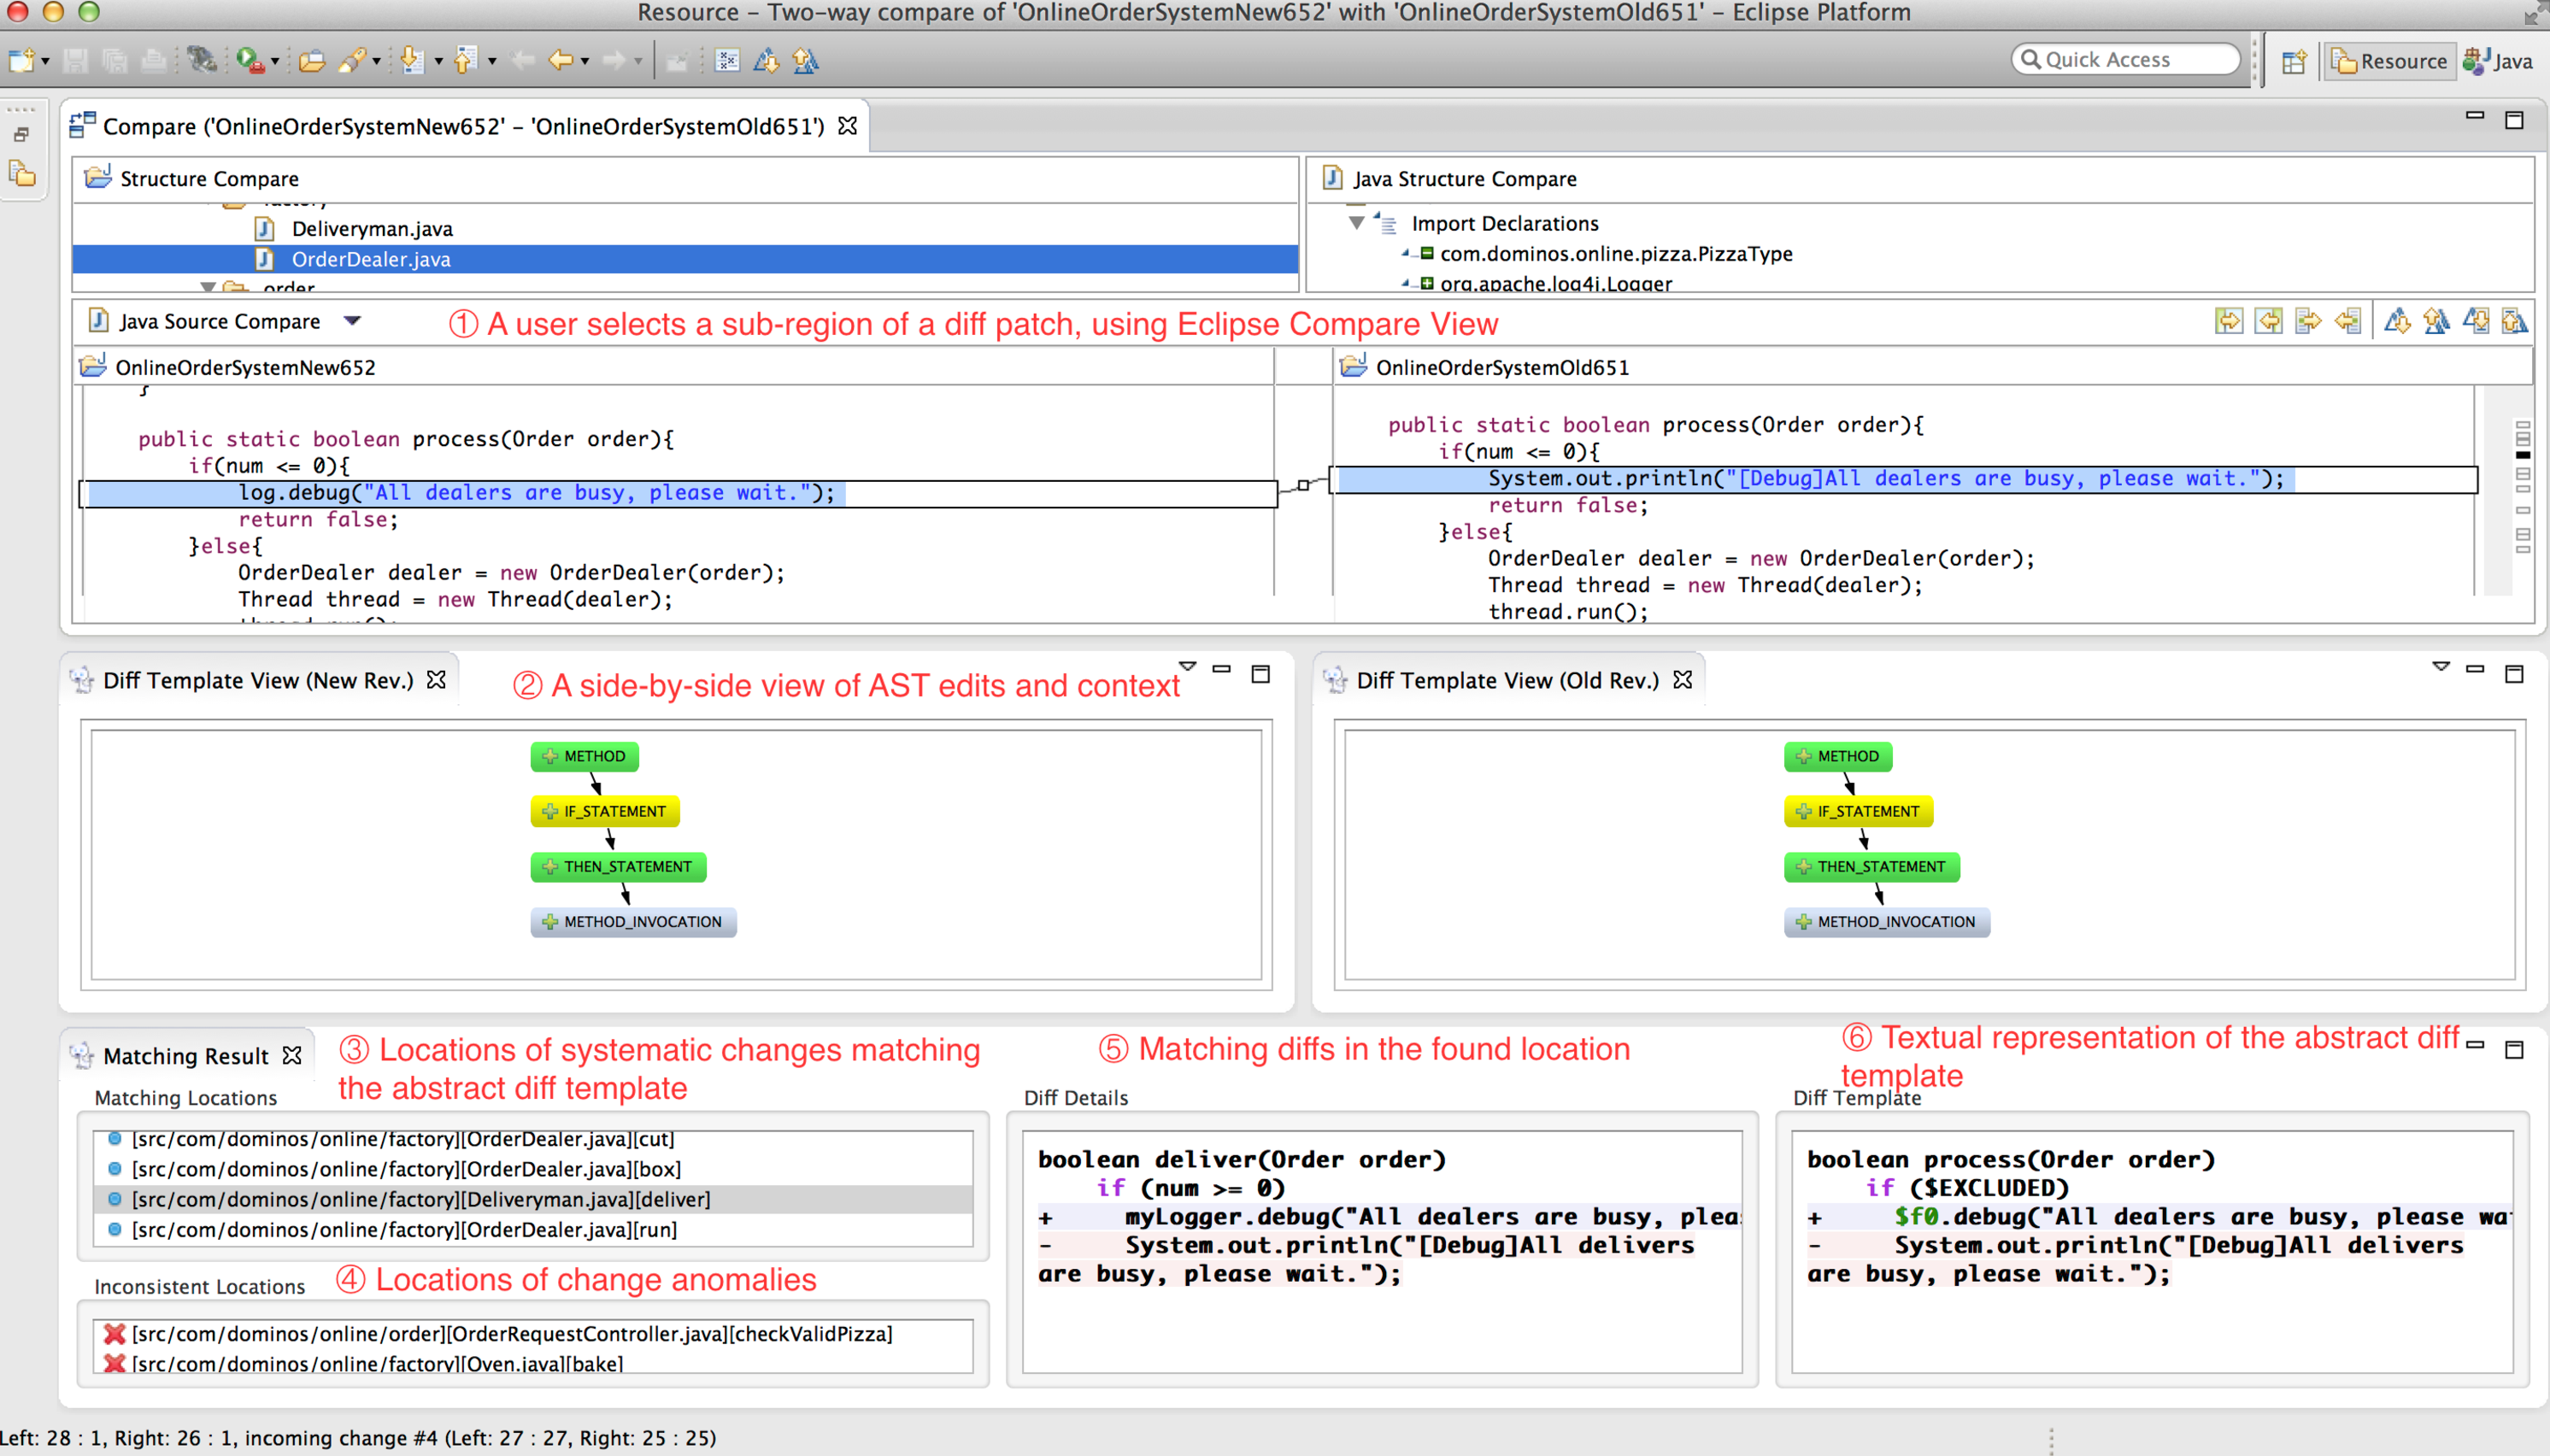
\includegraphics[width=\textwidth]{images/critics-UI.pdf}
 \caption{A screen snapshot of {\critics}'s Eclipse plugin and its features}
 \label{fig:critics-UI}
\end{figure}

Figure~\ref{fig:critics-UI} shows a screenshot of {\critics} plugin. {\critics} is integrated with the {\bf Compare View} in Eclipse, which displays line-level differences per file (see \ding{172} in Figure~\ref{fig:critics-UI}). A user can specify a program change she wants to inspect by selecting the corresponding code region in the Eclipse Compare View. The {\bf Diff Template View} (see \ding{173} in Figure~\ref{fig:critics-UI}) visualizes the change template of the selected change in a side-by-side view. Reviewers can parameterize concrete identifiers and exclude certain program statements by clicking on the corresponding node in the Diff Template View. {\bf Textual Diff Template View} (see \ding{177} in Figure~\ref{fig:critics-UI}) shows the change template in a unified format. The {\bf Matching Result View} summarizes the consistent changes as {\em similar changes} (see \ding{174} in Figure~\ref{fig:critics-UI}) and inconsistent ones as {\em anomalies} (see \ding{175} in Figure~\ref{fig:critics-UI}).
 

\subsection{Program Differencing} 
\label{sec:differencing} 
Program differencing serves as a basis for analyzing software changes between program versions. The program differencing problem is a dual problem of code matching, and is defined as follows. 
 
\indent{\textit{Suppose that a program $P'$ is created by modifying $P$. Determine the difference $\Delta$ between $P$ and $P'$. For a code fragment $c' \in P'$, determine whether $c' \in \Delta$. If not, find $c'$'s corresponding origin $c$ in $P.$}}

A code fragment in the new version either contributes to the difference or comes from the old version. If the code fragment has a corresponding origin in the old version, it means that it does not contribute to the difference. Thus, finding the delta between two versions is the same problem as finding corresponding code fragments between two versions. 

Suppose that a programmer inserts if-else statements in the beginning of the method \codefont{m\_A} and reorders several statements in the method \codefont{m\_B} without changing semantics (see Figure~\ref{fig:changeexample}). An intuitively correct matching technique should produce [(p0-c0), (p1-c2), (p2-c3), (p4-c4), (p4-c6), (p5-c7), (p6-c9), (p7-c8), (p8-c10), (p9-c11) ] and identify that c1 and c5 are added.  

\begin{figure*}
\centering
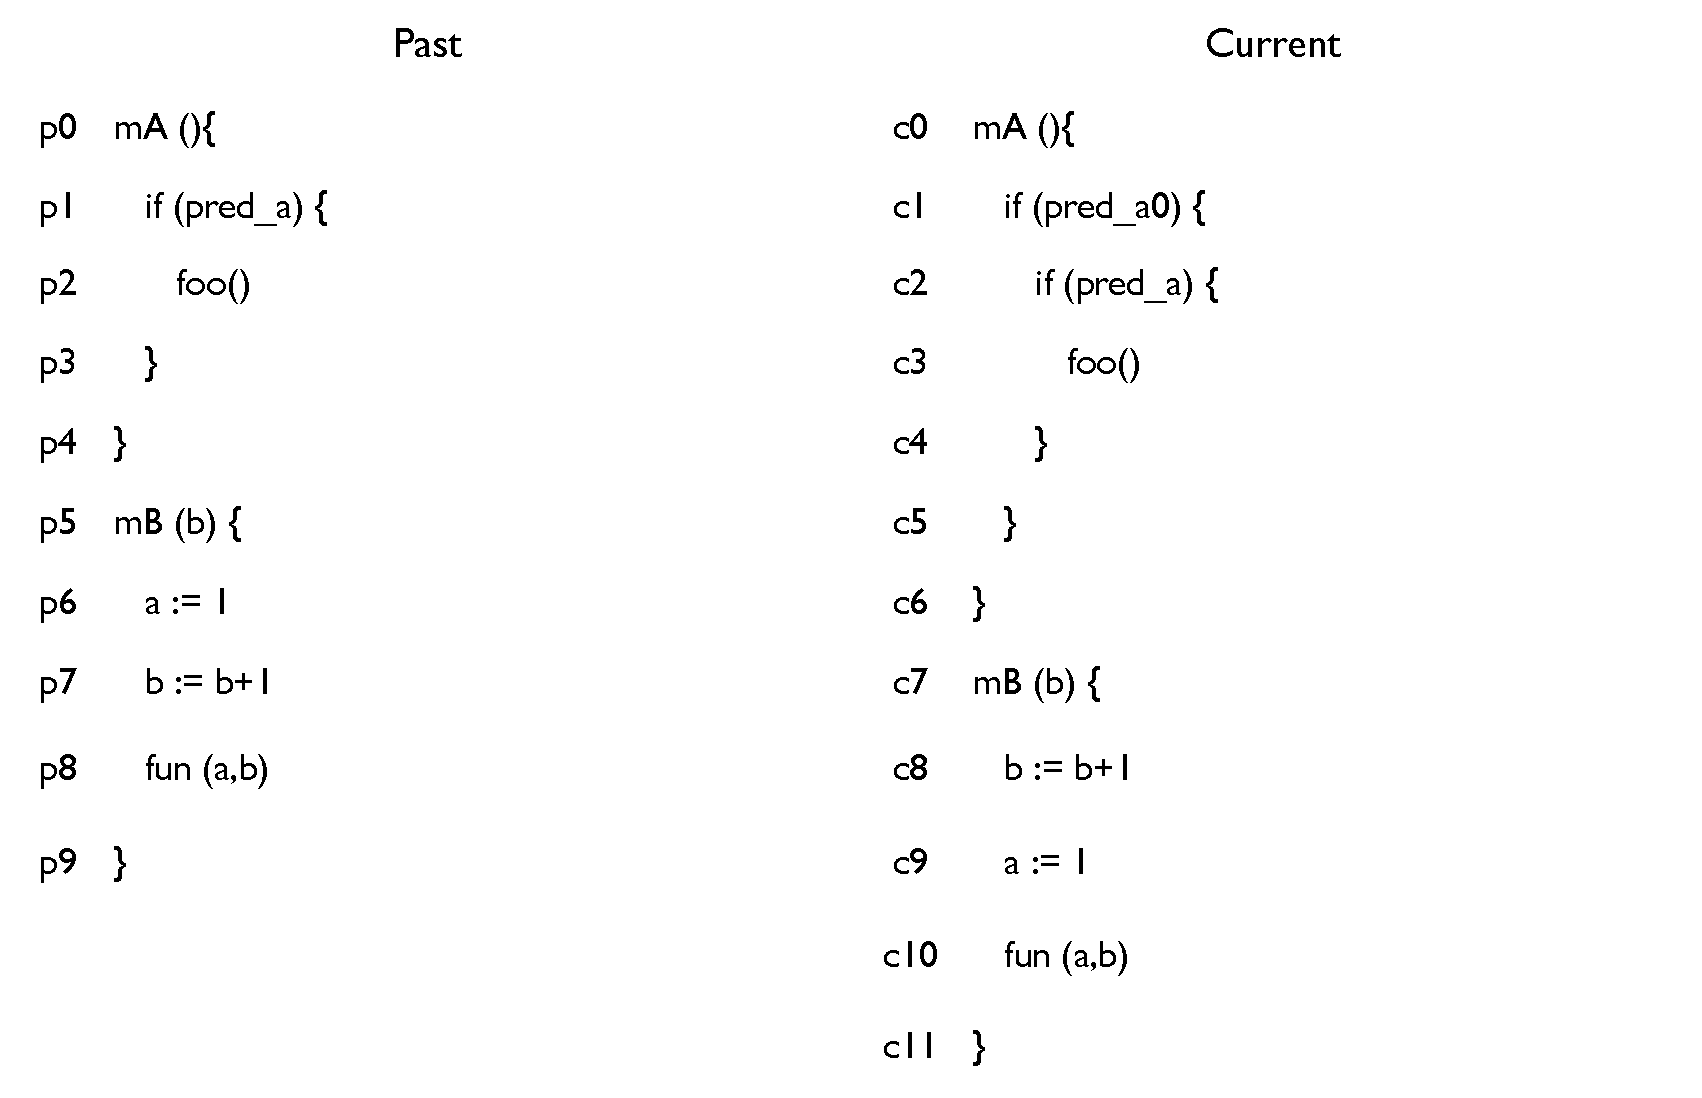
\includegraphics[width=0.95\textwidth]{images/DifferencingExample.pdf}
\caption{Example code change}
\label{fig:changeexample} 
\end{figure*}

Matching code across program versions poses several challenges. First, previous studies indicate that programmers often disagree about the origin of code elements; low inter-rater agreement suggests that there may be no ground truth in code matching~\cite{SKim2005}. Second, renaming, merging, and splitting of code elements that are discussed in the context of refactoring reconstruction in Section~\ref{sec:refactoringreview} make the matching problem non-trivial. Suppose that a file \codefont{PElmtMatch} changed its name to \codefont{PMatching}; a procedure \codefont{matchBlck} is split into two procedures \codefont{matchDBlck} and \codefont{matchCBlck}; and a procedure \codefont{matchAST} changed its name to \codefont{matchAbstractSyntaxTree}. The intuitively correct matching technique should produce [(\codefont{PElmtMatch, PMatching}), (\codefont{matchBlck, matchDBlck}), (\codefont{matchBlck, matchCBlck}), \\and (\codefont{matchAST, matchAbstractSyntaxTree})], while simple name-based matching will consider \codefont{PMatching}, \codefont{matchDBlck}, \codefont{matchCBlck}, and \codefont{matchAbstractSyntaxTree} added and consider \codefont{PElmtMatch}, \codefont{matchBlck}, and \codefont{matchAST} deleted.

Existing code matching techniques usually employ syntactic and textual similarity measures to match code. They can be characterized by the choices of (1) an underlying program representation, (2) matching granularity, (3) matching multiplicity, and (4) matching heuristics. Below, we categorize program differencing techniques with respect to internal program representations, and we discuss seminal papers for each representation.

\subsubsection{String and Lexical Matching.}
When a program is represented as a string, the best match between two strings is computed by finding the longest common subsequence (LCS) \cite{Apostolico1997}. The LCS problem is built on the assumption that (1) available operations are addition and deletion, and (2) matched pairs cannot cross one another. Thus, the longest common subsequence does not necessarily include all possible matches when available edit operations include copy, paste, and move. Tichy's \textit{bdiff} \cite{Tichy1984} extended the LCS problem by relaxing the two assumptions above: permitting crossing block moves and not requiring one-to-one correspondence. 


The line-level LCS implementation, \textit{diff} \cite{Hunt1977:LCS} is fast, reliable, and readily available. Thus, it has served as a basis for popular version control systems such as CVS. Many evolution analyses are based on {\it diff} because they use version control system data as input. For example, identification of fix-inducing code snippets is based on line tracking \textit{(file name:: function name:: line number)} backward from the moment that a bug is fixed~\cite{Sliwerski:2005} 

The longest common subsequence algorithm is a dynamic programming algorithm with $O(mn)$ in time and space, when $m$ is the line size of the past program and the $n$ is the line size of the current program. The goal of LCS-based diff is to report the minimum number of line changes necessary to convert one file to another. It consists of two phases: (1) computing the length of LCS and (2) reading out the longest common subsequence using a backtrace algorithm. Figure~\ref{fig:lcs} shows the pseudo code and the two dimensional array used to compute the LCS. Blue boxes mean the cells where the lines are identical. The red boxes represents the back trace of reading out the LCS, which produces the line matching of [(p0-c0), (p1-c1), (p2-c3), (p3-c5), (p4-c6), (p5-c7), (p6-c9), (p8-c10), (p9-c11) ]. Due to the assumption of no crossing matches, LCS does not find (p7-c8). In addition, because the matching is done at the line level and LCS does not consider the syntactic structure of code, it produces a line-level match such as (p3-c5) that do not observe the matching block parentheses rule. 

\begin{figure*}
\centering
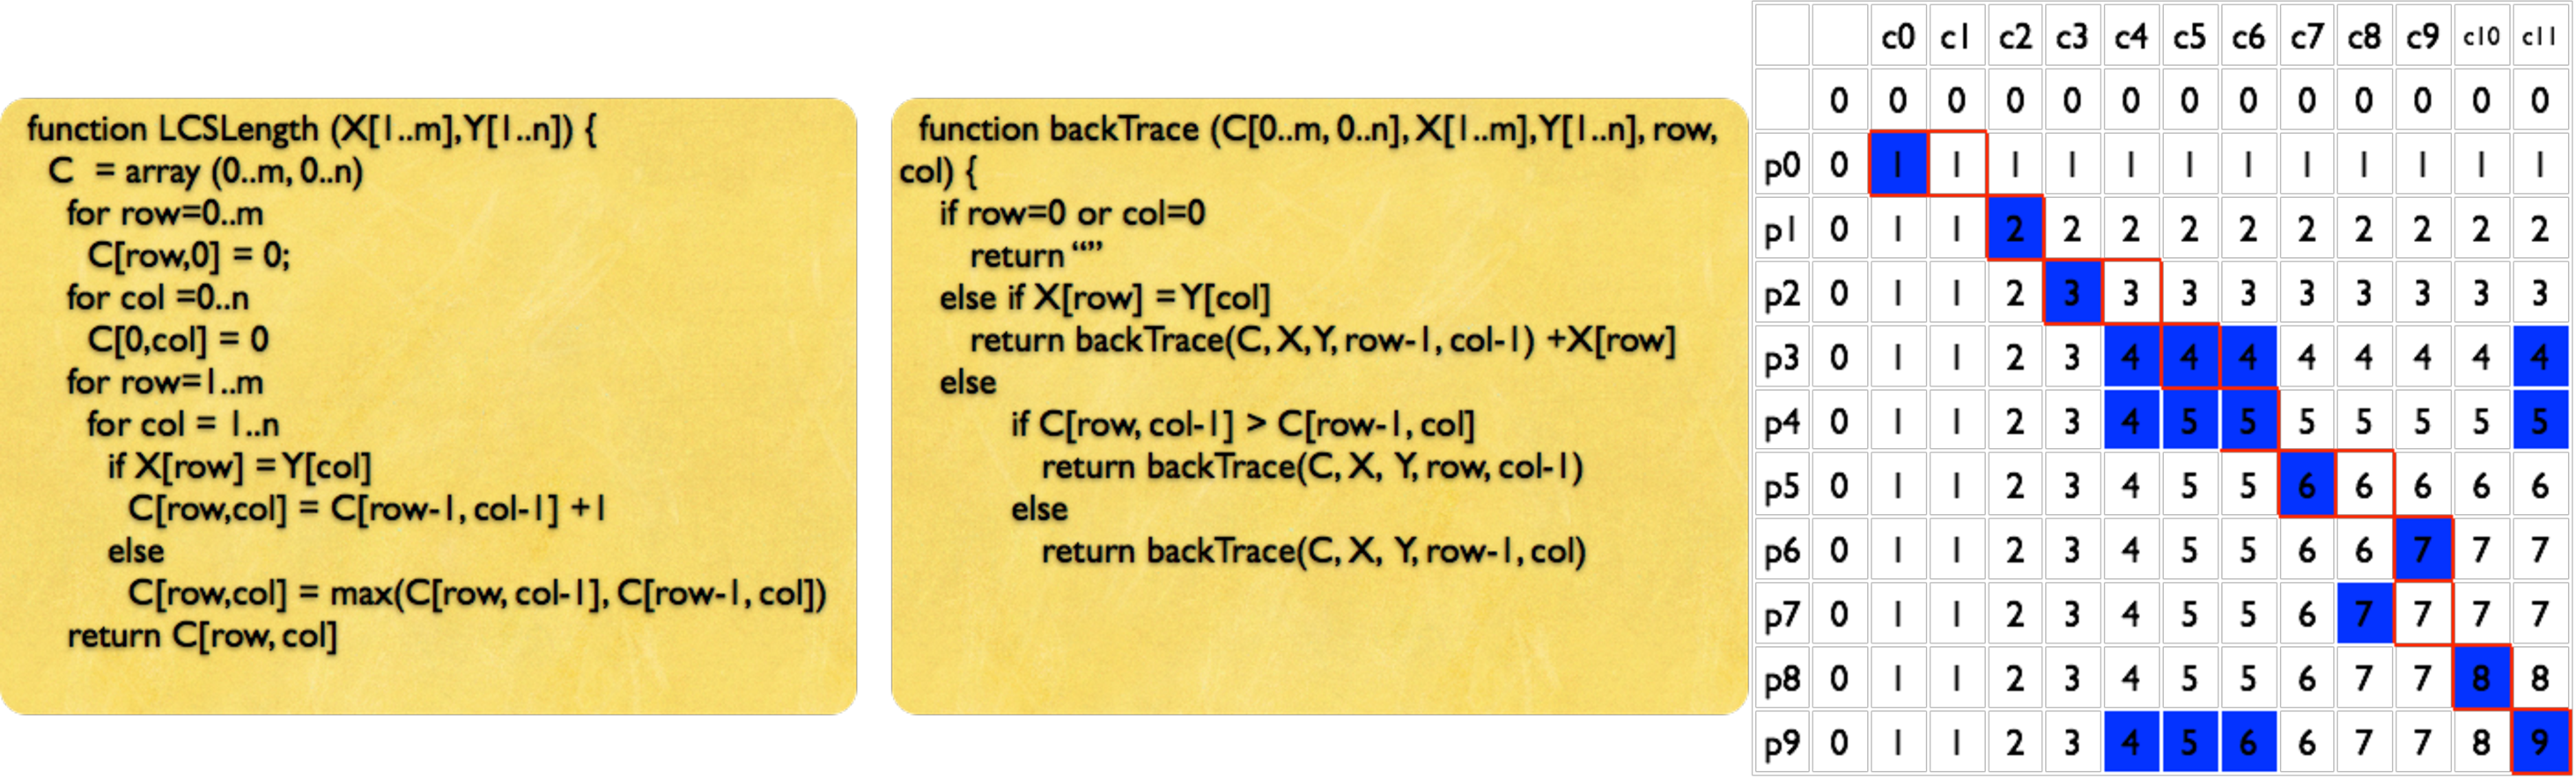
\includegraphics[width=0.95\textwidth]{images/LCS.pdf}
\caption{Longest common subsequence (LCS) algorithm and program differencing results based on LCS}
\label{fig:lcs} 
\end{figure*}

%Reiss \cite{Reiss2008} evaluated practical LCS-based source line tracking techniques. His investigation shows that the {\it W\_BEST\_LINE} method\textemdash  a variation of LCS algorithm that considers $k$ number of contextual lines\textemdash is about as effective as any other method but is faster and requires only a small amount of storage. This method compares each line to derive a normalized match value between zero (no match) and one (exact match); looks at a context consisting of $k/2$ lines before and after the line; and counts the number of these lines that match the corresponding line in the new version.  

% Canfora et al. 
%Recently, Canfora et al. \cite{Canfora2007} developed a source line technique that takes differencing results from {\it diff}-based version control systems as input and identifies changed-lines in addition to added- and deleted-lines. This technique first computes hunk similarity between every possible hunk pair using a vector space model and then computes the Levenstein distance \cite{Levenstein1966} to map source lines within the mapped hunk pairs. In contrast to {\it diff}, this approach detects changed-lines in addition to deleted- and added-lines. 

\subsubsection{Syntax Tree Matching.}
For software version merging, Yang~\cite{Yang1991} developed an AST differencing algorithm. Given a pair of functions $(f_T,f_R)$, the algorithm creates two abstract syntax trees $T$ and $R$ and attempts to match the two tree roots. Once the two roots match, the algorithm aligns $T$'s subtrees ${t_1, t_2, ..., t_i}$ and $R$'s subtrees ${r_1, r_2, ... r_j}$ using the LCS algorithm and maps subtrees recursively. This type of tree matching respects the parent-child relationship as well as the order between sibling nodes, but is very sensitive to changes in nested blocks and control structures because tree roots must be matched for every level. Figure~\ref{fig:AST} shows the abstract tree representations of the code example shown in Figure~\ref{fig:changeexample}. Figure~\ref{fig:YangDiff} shows its AST differencing algorithm in pseudo-code and the differencing results.  Because the algorithm respects parent-child relationships when matching code, all matches are observe the syntactic boundary of code and  the matching block parentheses rule. Similar to LCS, because Yang's algorithm aligns subtrees at the current level by LCS, it cannot find crossing matches caused by code reordering. Furthermore, the algorithm is very sensitive to tree level changes or insertion of new control structures in the middle, because Yang's algorithm performs top-down AST matching. 

\begin{figure*}
\centering
\begin{minipage}{.45\textwidth}
  \centering
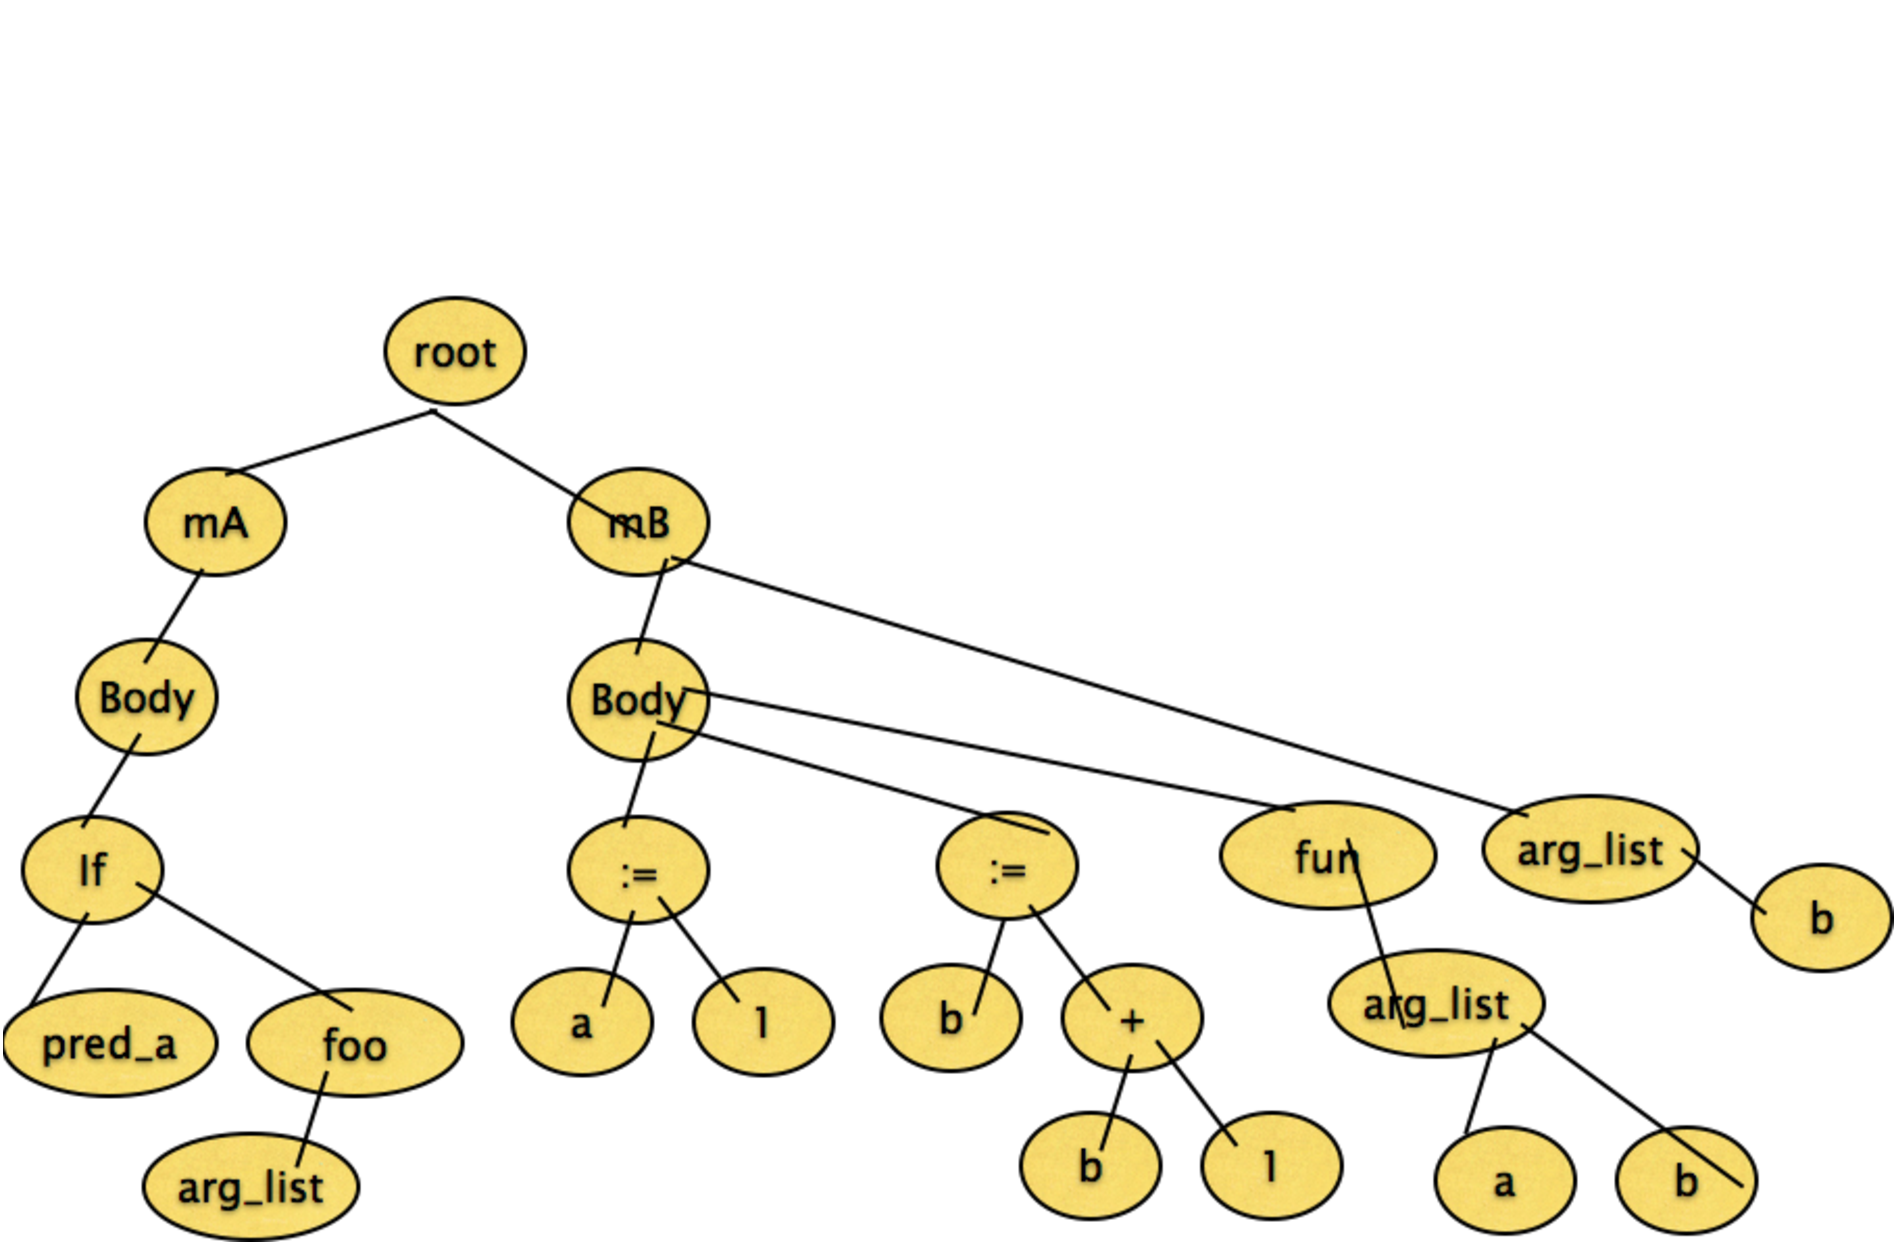
\includegraphics[width=0.9\textwidth]{images/PastAST.pdf}
\end{minipage}
\begin{minipage}{.45\textwidth}
  \centering
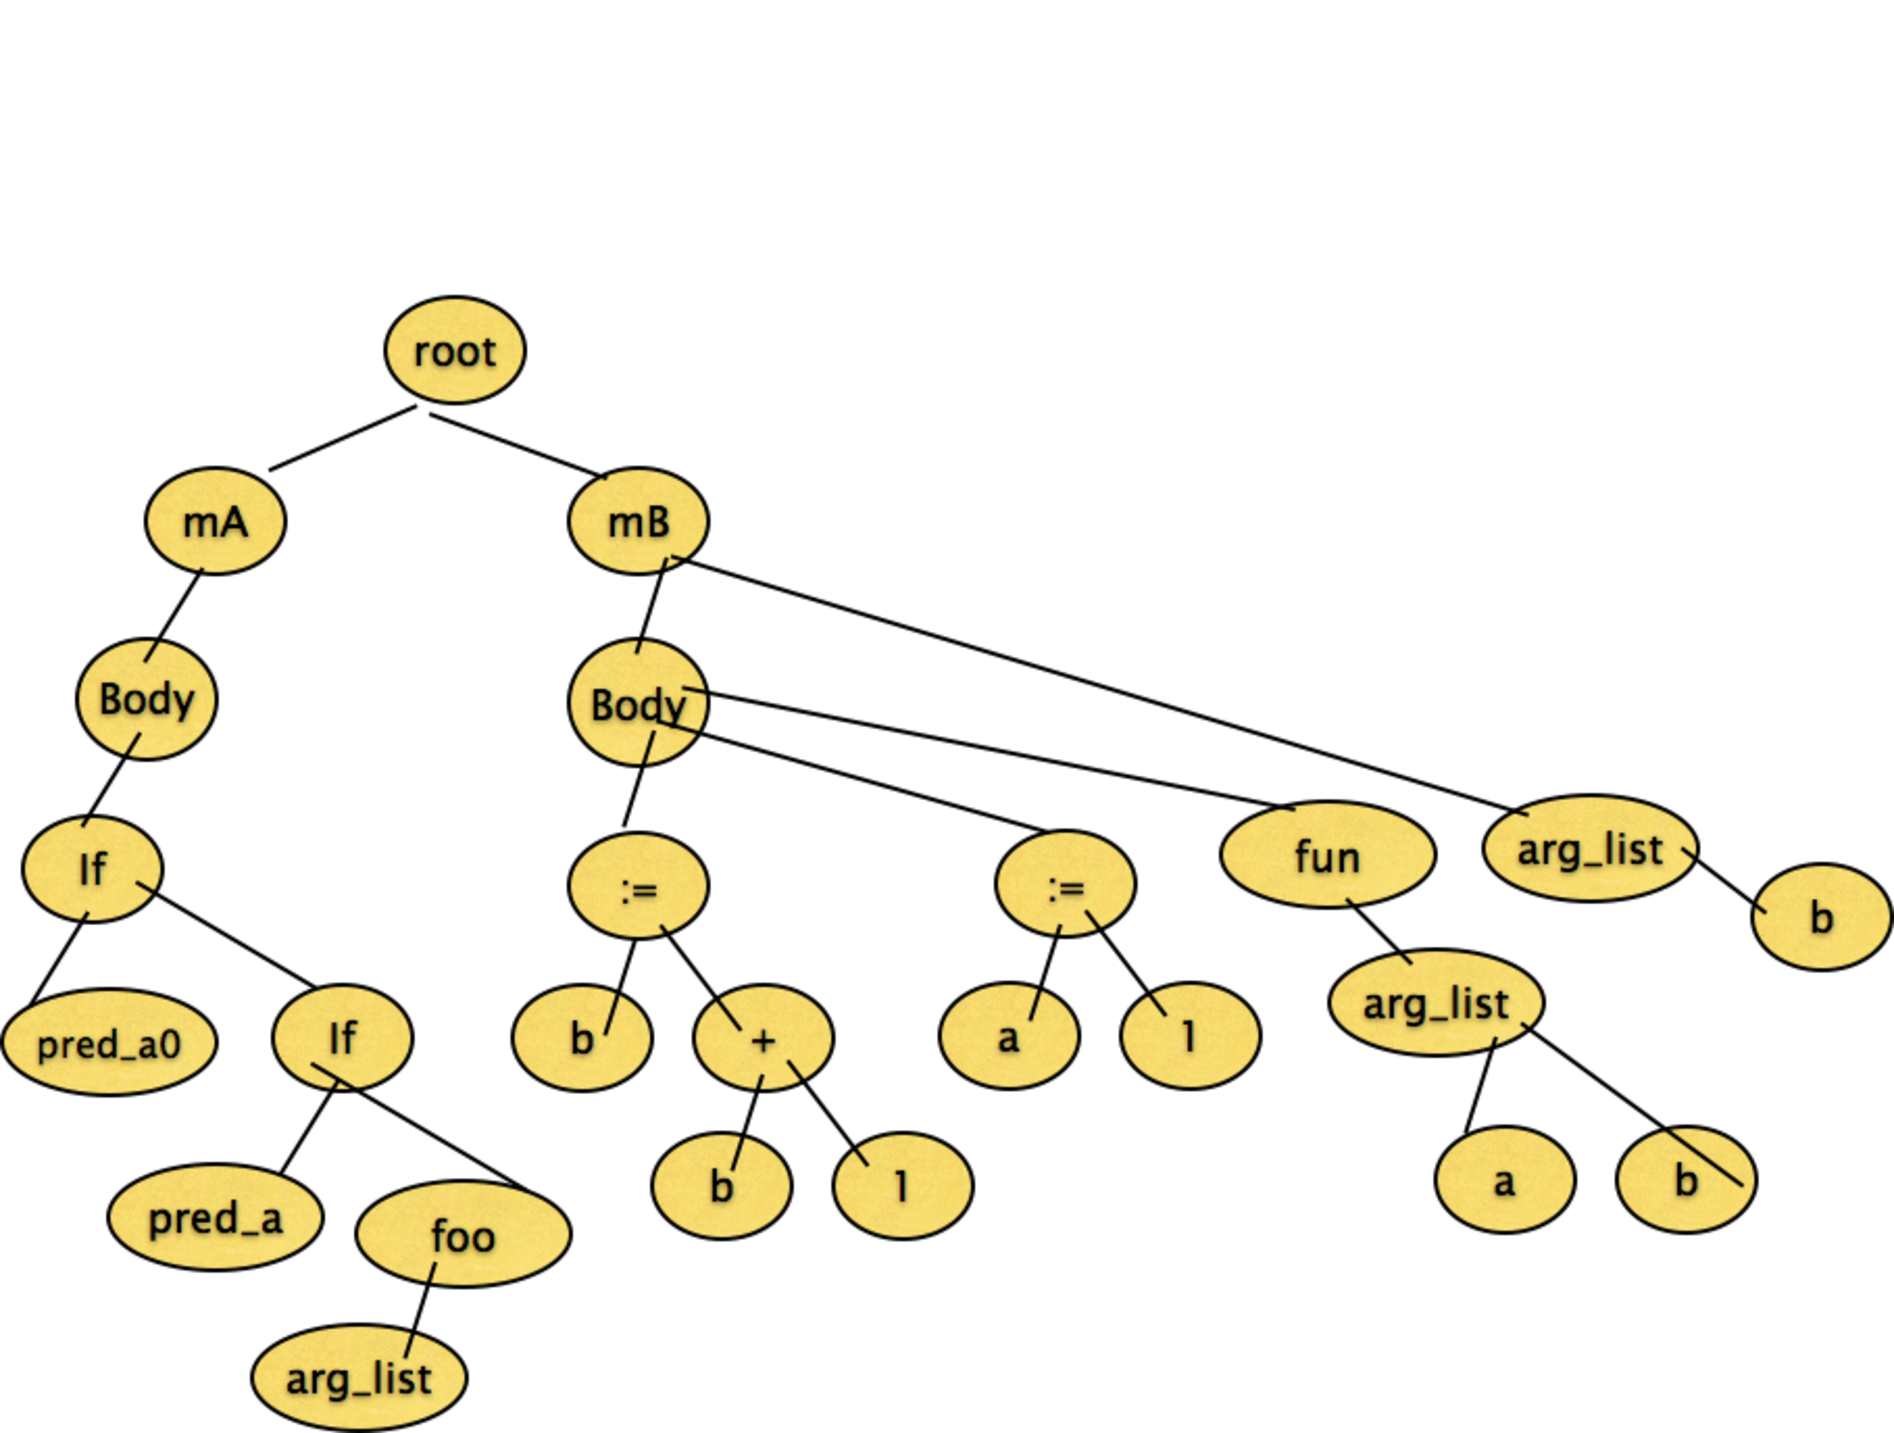
\includegraphics[width=0.9\textwidth]{images/CurrentAST.pdf}
\end{minipage}
\caption{Abstract Syntax Tree: Past (left) and Current (right)} 
\label{fig:AST} 
\end{figure*}

\begin{figure*}
\centering
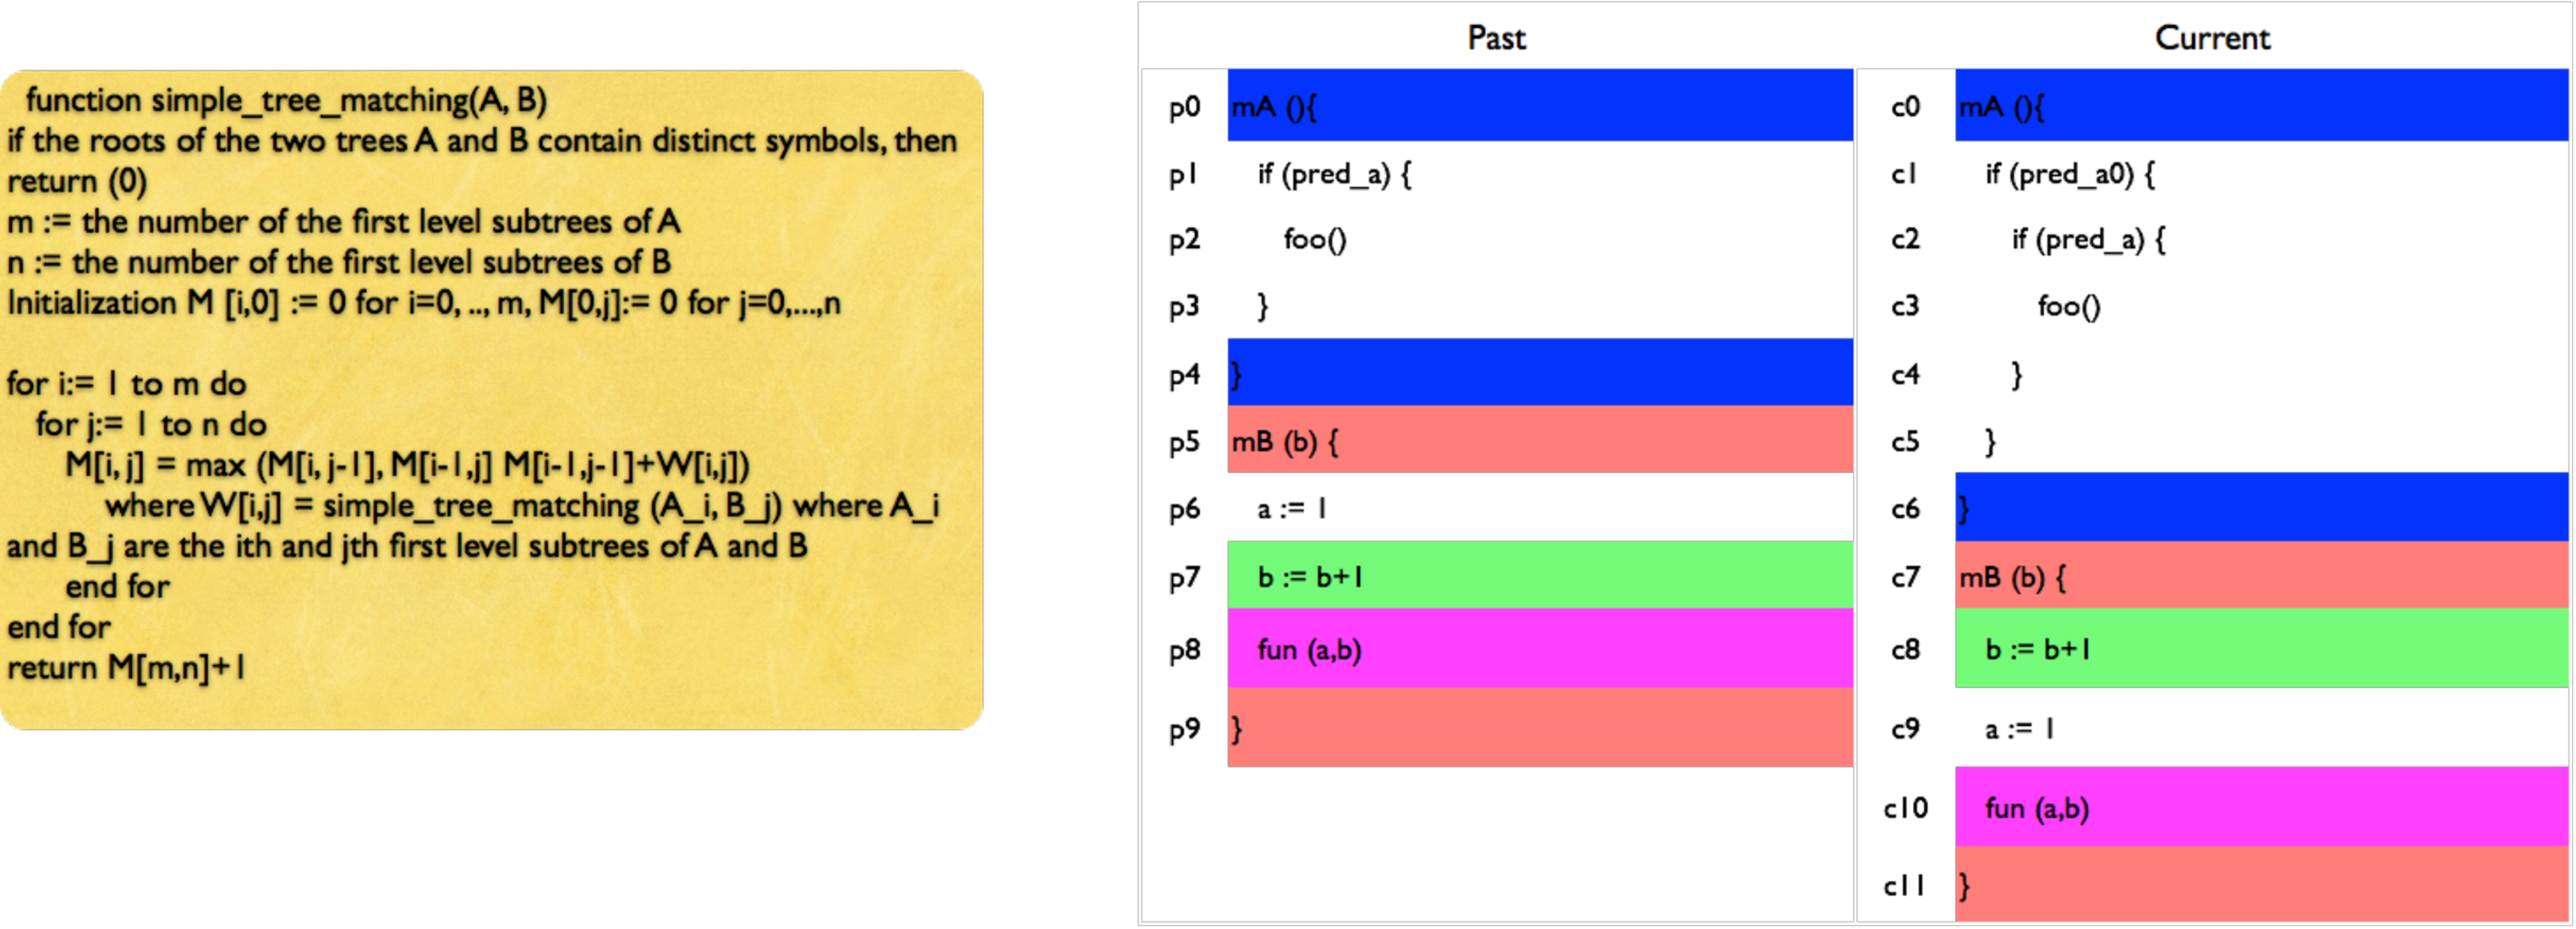
\includegraphics[width=0.95\textwidth]{images/Yang.pdf}
\caption{Yang's Abstract Syntax Tree differencing algorithm and results} 
\label{fig:YangDiff} 
\end{figure*}

%For dynamic software updating, Neamtiu et al. \cite{Neamtiu2005} built an AST-based algorithm that tracks simple changes to variables, types, and functions. Neamtiu's algorithm assumes that function names are relatively stable over time.  It traverses two ASTs in parallel; matches the ASTs of functions with the same name; and incrementally adds one-to-one mappings as long as the ASTs have the same shape. In contrast to Yang's algorithm, it cannot compare structurally different ASTs. 

% Change Distiller 
As another example, Change Distiller~\cite{FWP2007} uses an improved version of Chawathe et al.'s hierarchically structured data comparison algorithm \cite{Chawathe1996}. Change Distiller takes two abstract syntax trees as input and computes basic tree edit operations such as {\it insert, delete, move} or {\it update} of tree nodes. It uses {\it bi-gram string similarity} to match source code statements such as method invocations and uses {\it subtree similarity} to match source code structures such as if-statements. After identifying tree edit operations, Change Distiller maps each tree-edit to an atomic AST-level change type. 

% R. Walker Cottrell et al.'s Breakaway \cite{Cottrell:2007} automatically identifies detailed structural correspondences between two abstract syntax trees to help programmers generalize two pieces of similar code. Its two-pass greedy algorithm is applied to ordered child list properties (statements in a block) then to unordered nodes (method declarations). 

% Finally, the following two techniques do not directly compare ASTs but use syntactic information to guide string level differencing.  Hunt and Tichy's 3-way merging tool \cite{Hunt2002} parses a program into a language neutral form; compares token strings using the LCS algorithm; and finds syntactic changes using structural information from the parse. Raghavan et al.'s Dex \cite{Raghavan:2004:Dex} locates the changed parts in C source code files using {\it patch} file information and feeds the changed parts into a tree differencing algorithm to output the edit operations. 

\subsubsection{Control Flow Graph Matching.}
Laski and Szermer \cite{Laski1992} first developed an algorithm that computes one-to-one correspondences between CFG nodes in two programs. This algorithm reduces a CFG to a series of single-entry, single-exit subgraphs called hammocks and matches a sequence of hammock nodes using a depth first search (DFS). Once a pair of corresponding hammock nodes is found, the hammock nodes are recursively expanded in order to find correspondences within the matched hammocks. 
 
\textit{Jdiff} \cite{Apiwattanapong2004} extends Laski and Szermer's (LS) algorithm to compare Java programs based on an enhanced control flow graph (ECFG). \textit{Jdiff} is similar to the LS algorithm in the sense that hammocks are recursively expanded and compared, but is different in three ways: First, while the LS algorithm compares hammock nodes by the name of a start node in the hammock, \textit{Jdiff} checks whether the ratio of unchanged-matched pairs in the hammock is greater than a chosen threshold in order to allow for flexible matches. Second, while the LS algorithm uses DFS to match hammock nodes, \textit{Jdiff} only uses DFS up to a certain look-ahead depth to improve its performance. Third, while the LS algorithm requires hammock node matches at the same nested level, \textit{Jdiff} can match hammock nodes at a different nested level; thus, \textit{Jdiff} is more robust to addition of while loops or if-statements at the beginning of a code segment. \textit{Jdiff} has been used for regression test selection \cite{Orso2004} and dynamic change impact analysis \cite{Apiwattanapong2005}. Figure~\ref{fig:JDiff} shows the code example and corresponding extended control flow graph representations in Java. Because their representation and matching algorithm is designed to account for dynamic dispatching and exception handling, it can detect changes in the method body of \codefont{m3 (A a)}, even though it did not have any textual edits: (1) \codefont{a.m1()} calls the method definition \codefont{B.m()} for the receiver object of type B and (2) when the exception type \codefont{E3} is thrown, it is caught by the catch block \codefont{E1} instead of the catch block \codefont{E2}.   

\begin{figure*}
\centering
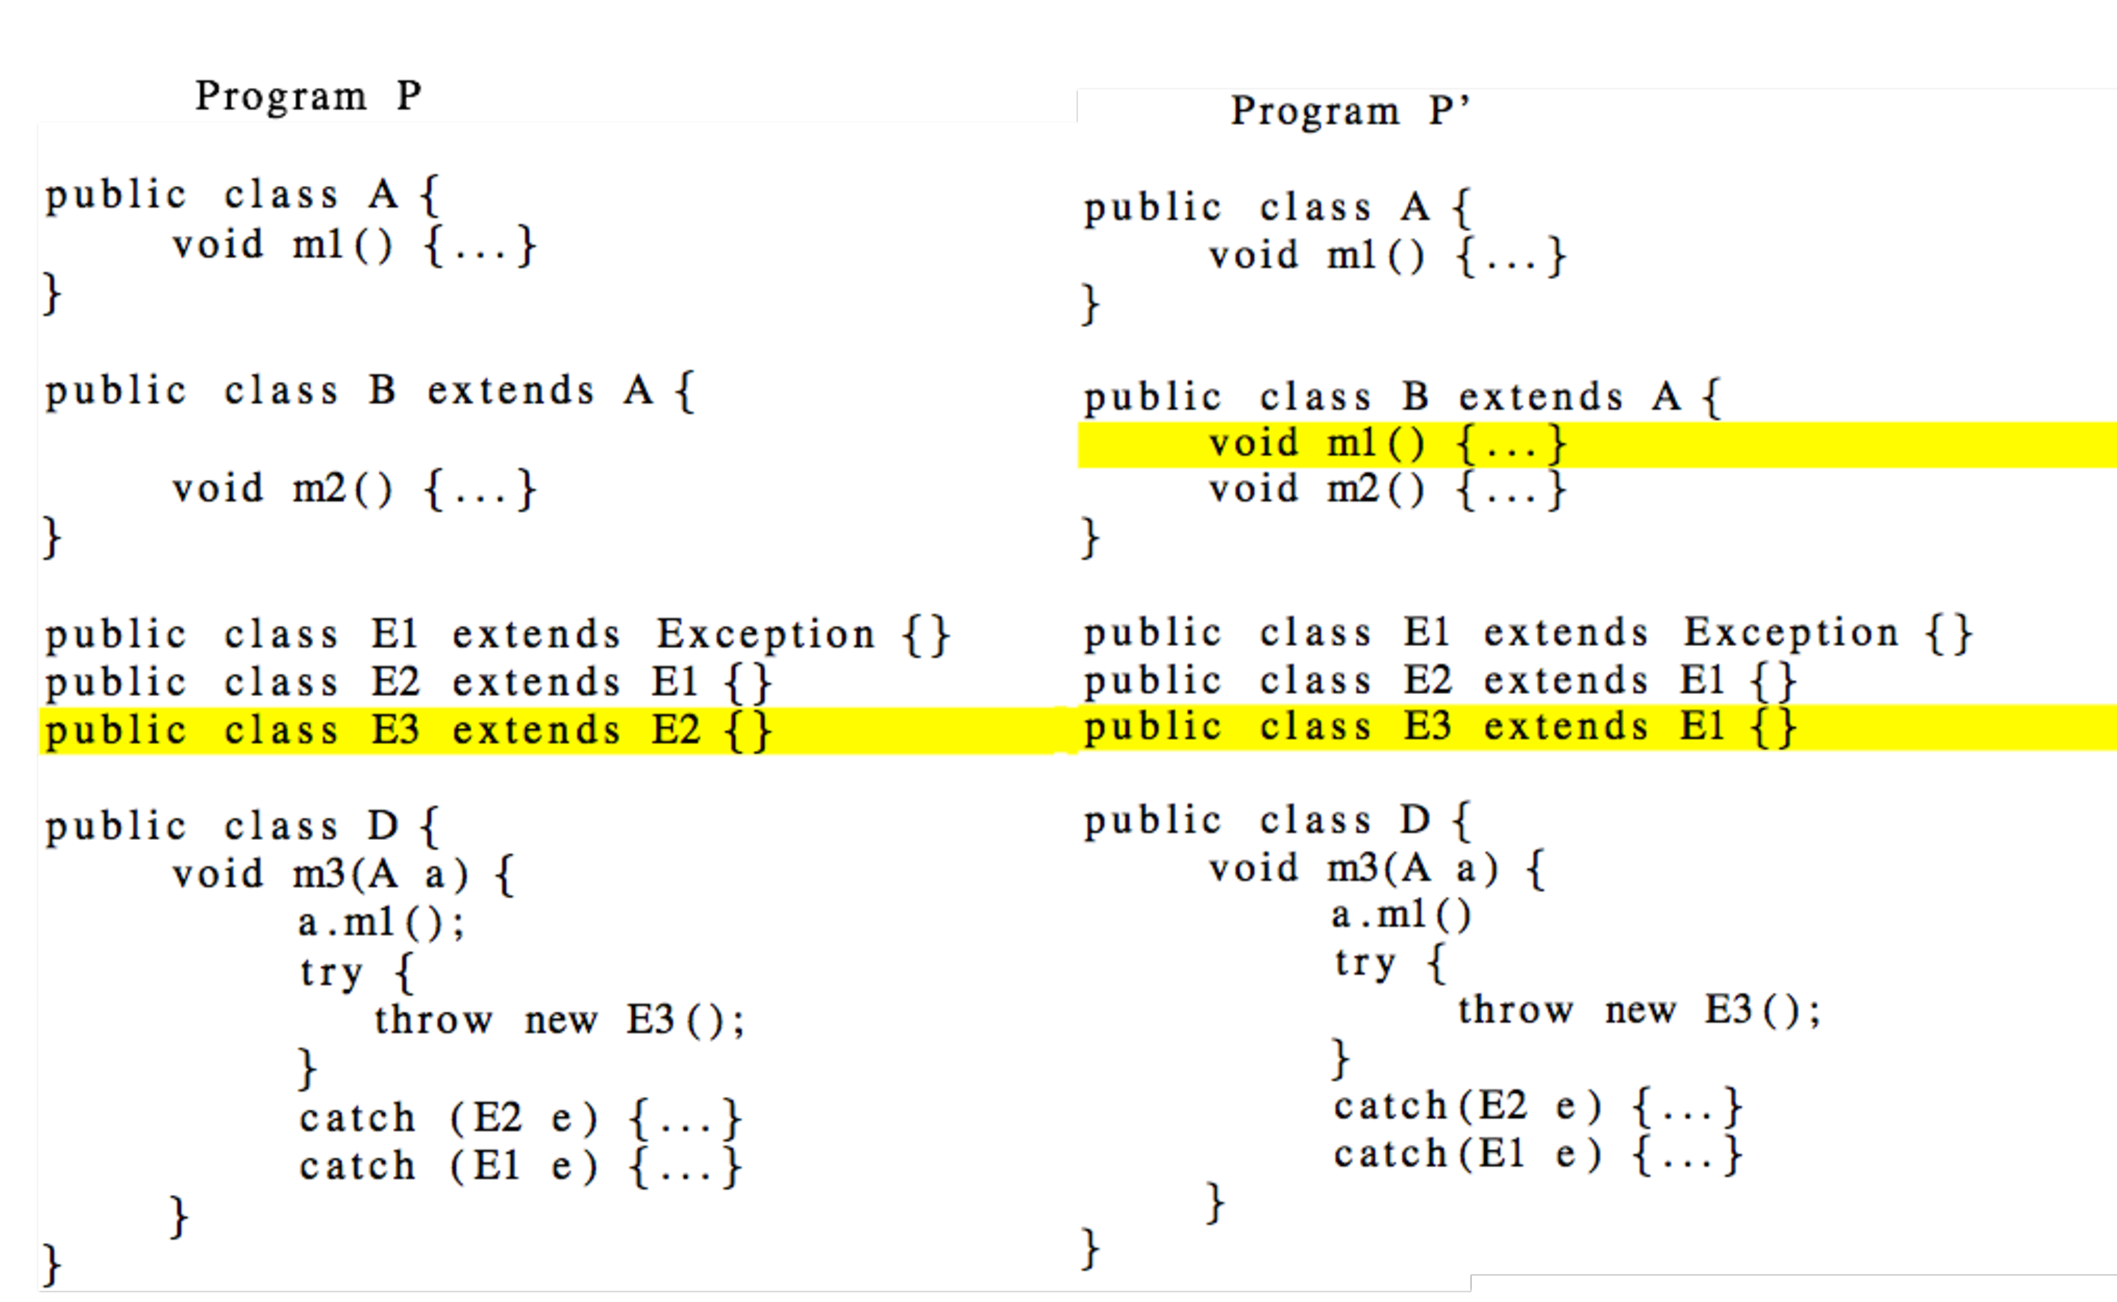
\includegraphics[width=0.95\textwidth]{images/JDiffCodeExample.pdf}
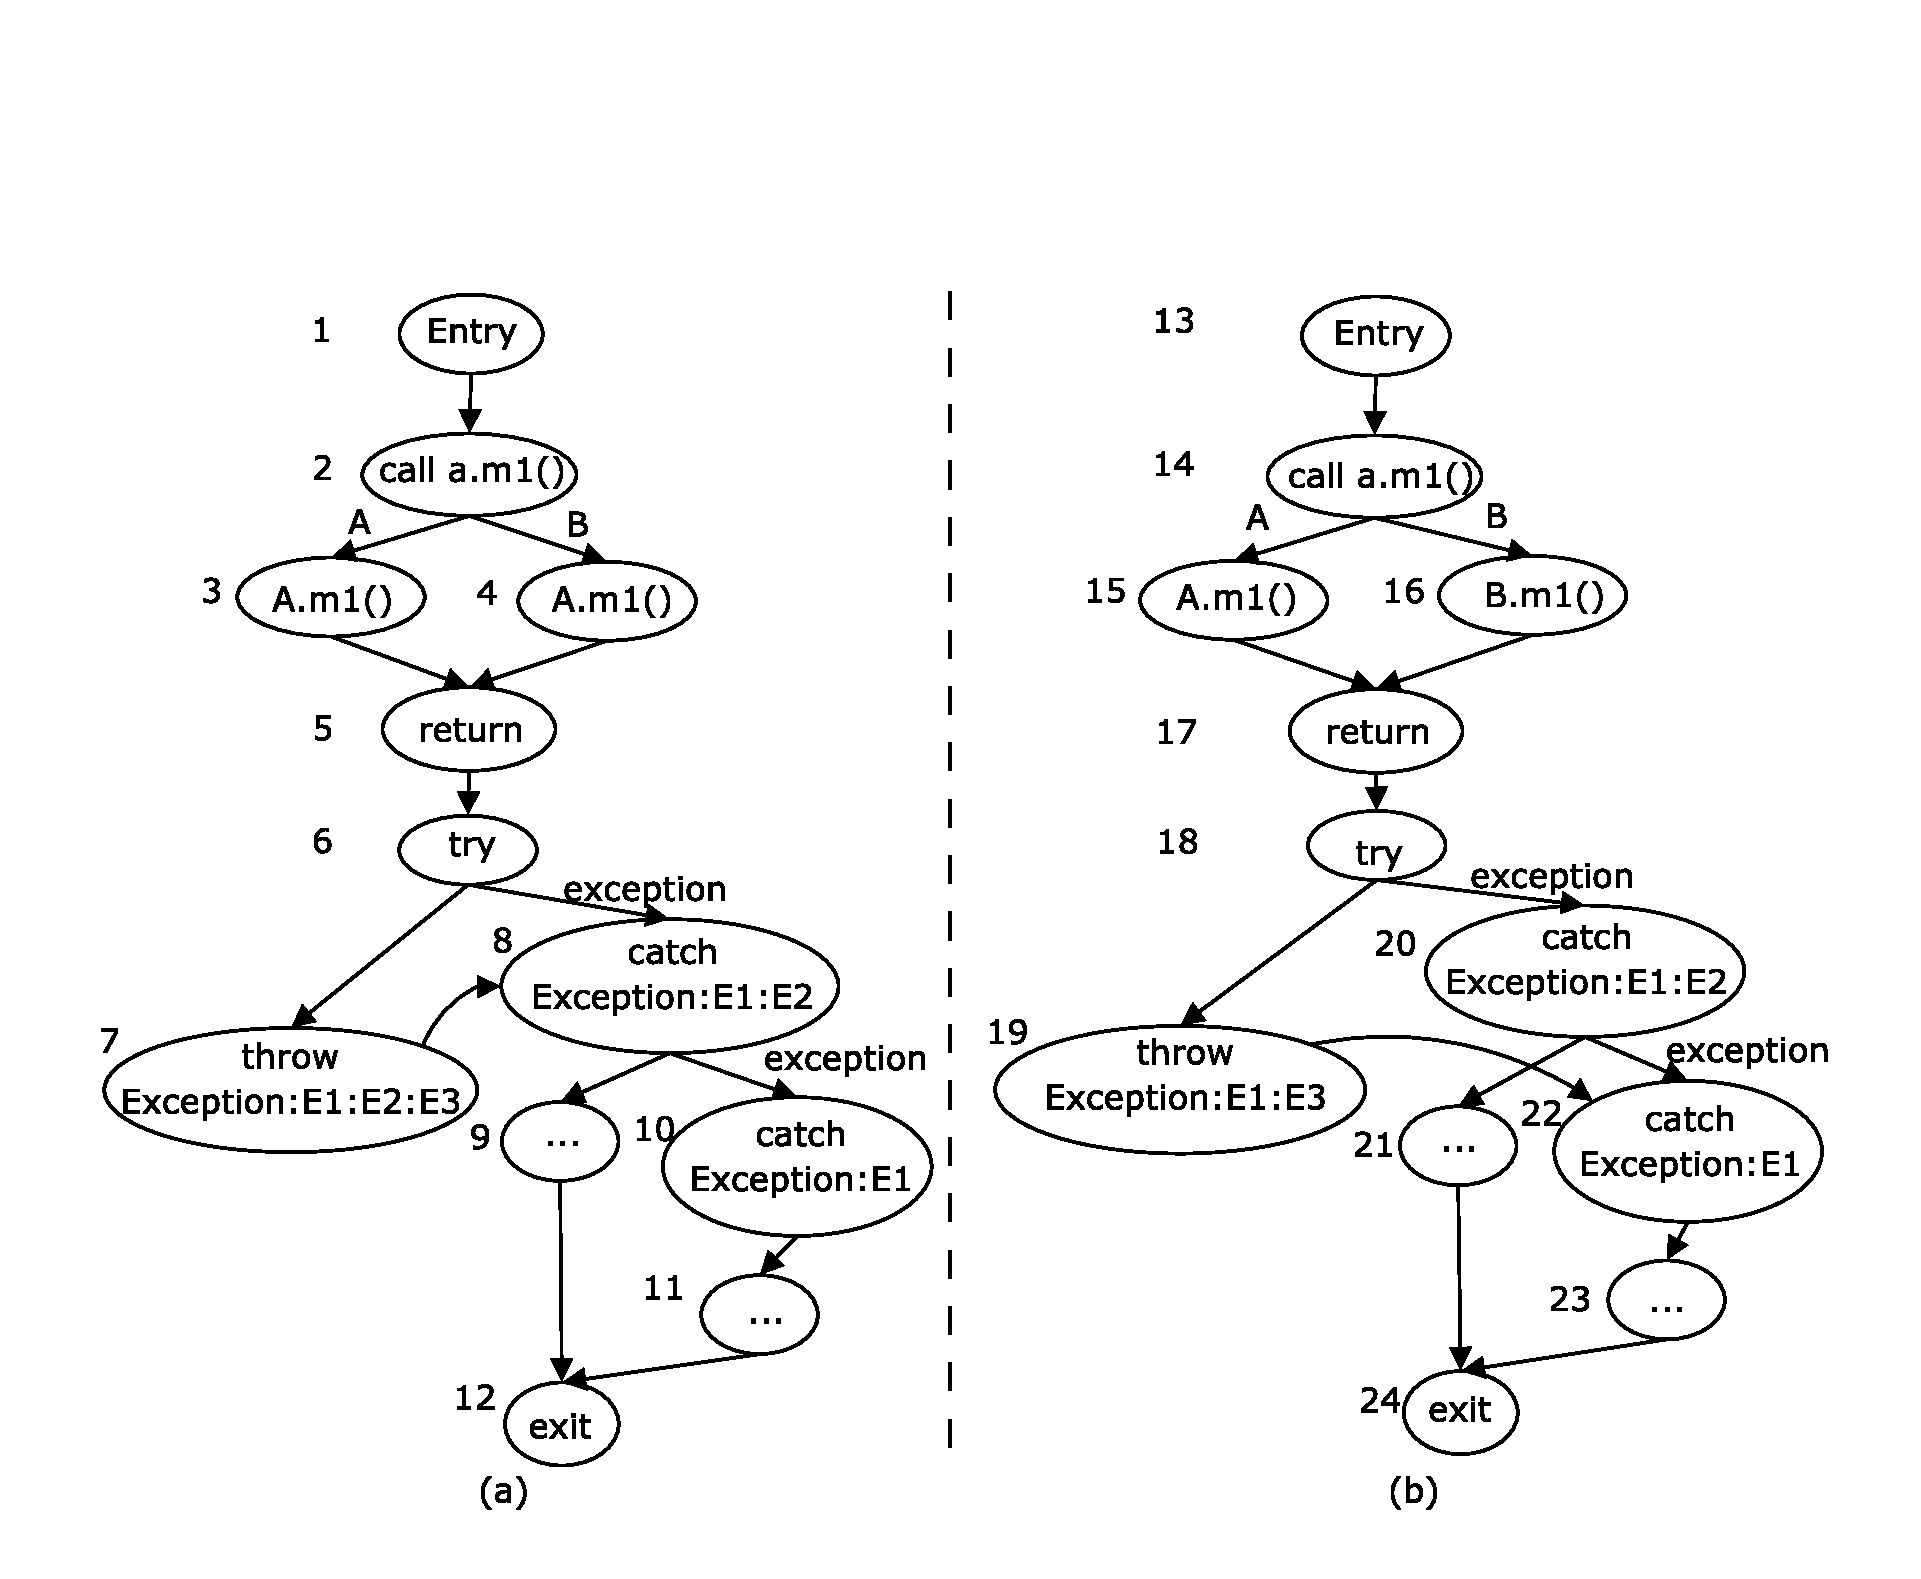
\includegraphics[width=0.95\textwidth]{images/JDiffCFG.pdf}
\caption{JDiff Change Example and CFG representations~\cite{Apiwattanapong2005}} 
\label{fig:JDiff} 
\end{figure*}

CFG-like representations are commonly used in regression test selection research. Rothermel and Harrold \cite{Rothermel1997} traverse two CFGs in parallel and identify a node with unmatched edges, which indicates changes in code. In other words, their algorithm stops parallel traversal as soon as it detects changes in a graph structure; thus, this algorithm does not produce deep structural matches between CFGs. However, traversing graphs in parallel is still sufficient for the regression testing problem because it conservatively identifies affected test cases. In practice, regression test selection algorithms~\cite{Harrold2001, Orso2004} require that syntactically changed classes and interfaces are given as input to the CFG matching algorithm. 

\subsubsection{Program Dependence Graph Matching.}
There are several program differencing algorithms based on a program dependence graph \cite{Horwitz1990, Binkley1995, Jackson1994}. 

Horwitz \cite{Horwitz1990} presents a semantic differencing algorithm that operates on a program representation graph (PRG) which combines features of program dependence graphs and static single assignment forms. In her definition, semantic equivalence between two programs $P1$ and $P2$ means that, for all states $\sigma$ such that $P1$ and $P2$ halt, the sequence of values produced at $c1$ is identical to the sequence of values produced at $c2$ where $c1$ and $c2$ are corresponding locations. 
Horwitz uses Yang's algorithm \cite{Yang1989} to partition the vertices into a group of semantically equivalent vertices based on three properties, (1) the equivalence of their operators, (2) the equivalence of their inputs, (3) the equivalence of the predicates controlling their evaluation. The partitioning algorithm starts with an initial partition based on the operators used in the vertices. Then by following flow dependence edges, it refines the initial partition if the successors of the same group are not in the same group. Similarly, it further refines the partition by following control dependence edges. If two vertices in the same partition are textually different, they are considered to have only a {\it textual change}. If two vertices are in different partitions, they have a {\it semantic change}. After the partitioning phase, the algorithm finds correspondences between $P1$'s vertices and $P2$'s vertices that minimize the number of semantically or textually changed components of $P2$. 
% semantic change: no matching partition. 
% textual change: same partition but different text. 
% same: same partition and same text. 
In general, PDG-based algorithms are not applicable to popular modern program languages because they can run only on a limited subset of C-like languages without global variables, pointers, arrays, or procedures. 

%Binkley et al. \cite{Binkley1995} presents a 3-way merging algorithm that is based on semantic differences. This algorithm does not find corresponding elements between two versions of a program, but rather makes an assumption that a special editor is used to tag each PDG node to identify added nodes, deleted nodes and changed nodes. Given PDG node level correspondence among three input programs A, B, and Base, the integration algorithm produces a program M that integrates the difference A from Base, the difference B from Base, and the preserved behavior among A, B, and Base. The behavior differences between A and B are approximated by the slice of $AP_{A,Base}$ in $G_A$ where $AP_{A,Base}$ is a set of vertices of $G_A$ whose program slice is different from $G_{Base}$'s slice. Although the problem of determining  whether $G_M$ corresponds to some program is NP-complete, Binkley et al. presented a backtracking algorithm that behaves satisfactorily on actual programs. 

\subsubsection{Related Topics: Model Differencing and Clone Detection.} 

A clone detector is simply an implementation of an arbitrary equivalence function. The equivalence function defined by each clone detector depends on a program representation and a comparison algorithm. Most clone detectors are heavily dependent on (1) hash functions to improve performance, (2) parametrization to allow flexible matches, and (3) thresholds to remove spurious matches. A clone detector can be considered as a many-to-many matcher based solely on content similarity heuristics. 

In addition to these, several differencing algorithms compare model elements~\cite{UMLDiff2005, Ohst2003:umldiff, Soto2006:deltaprocess, Duley2012:vdiff}. For example, UMLdiff~\cite{UMLDiff2005} matches methods and classes between two program versions based on their name. However, these techniques assume that no code elements share the same name in a program and thus use name similarity to produce one-to-one code element matches. Some have developed a general, meta-model based, configurable program differencing framework~\cite{Schmidt2008:sidiff, EMF}. For example, SiDiff \cite{Schmidt2008:sidiff,Treude2007} allows tool developers to configure various matching algorithms such as identity-based matching, structure-based matching, and signature-based matching by defining how different types of elements need to be compared and by defining the weights for computing an overall similarity measure.


 

\subsection{Recording Changes: Edit Capture and Replay} 
\label{sec:record} 
Recorded change operations can be used to help programmers reason about software changes. Several editors or integrated development environment (IDE) extensions capture and replay keystrokes, editing operations, and high-level update commands to use the recorded change information for intelligent version merging, studies of programmers' activities, and automatic updates of client applications. When recorded change operations are used for helping programmers reason about software changes, this approach's limitation depends on the granularity of recorded changes. If an editor records only keystrokes and basic edit operations such as cut and paste, it is a programmer's responsibility to raise the abstraction level by grouping keystrokes. If an IDE records only high-level change commands such as refactorings, programmers cannot retrieve a complete change history. In general, capturing change operations to help programmers reason about software change is {\it impractical} as this approach constrains programmers to use a particular IDE.  Below, we discuss a few examples of recording change operations from IDEs:  

Spyware is a representative example in this line of work~\cite{Robbes2008:spyware}. It is a smalltalk IDE extension to capture AST-level change operations (creation, addition, removal and property change of an AST node) as well as refactorings. It captures refactorings during development sessions in an IDE rather than trying to infer refactorings from two program versions. Spyware is used to study when and how programmers perform refactorings, but such edit-capture-replay could be used for performing refactoring-aware version merging~\cite{Dig2007} or updating client applications due to API evolution~\cite{Henkel2005}. %  that  automatically resolves merging conflicts that a regular {\it diff}-based merging algorithm cannot resolve by taking into account the semantics of recorded move and rename refactorings~\cite{Dig2007}. CatchUp \cite{Henkel2005} captures API refactoring actions as a developer evolves an API and allows the users of the API to replay the refactorings to bring their client software up to date. 

%Evans et al. \cite{Evans2003} collected students' programming data by capturing keystroke, mouse and window focus events generated from the Windows operating system and used this data to observe programming practices. Similarly, Kim et al.~\cite{Kim04} studied copy and paste programming practices by recording keystrokes and edit operations in an Eclipse IDE. 
% granularity -> limitations 

 

\section{An Organized Tour of Seminal Papers: III. Change Validation} 
\label{sec:debugtest}
\begin{figure}[ht]
 \centering
 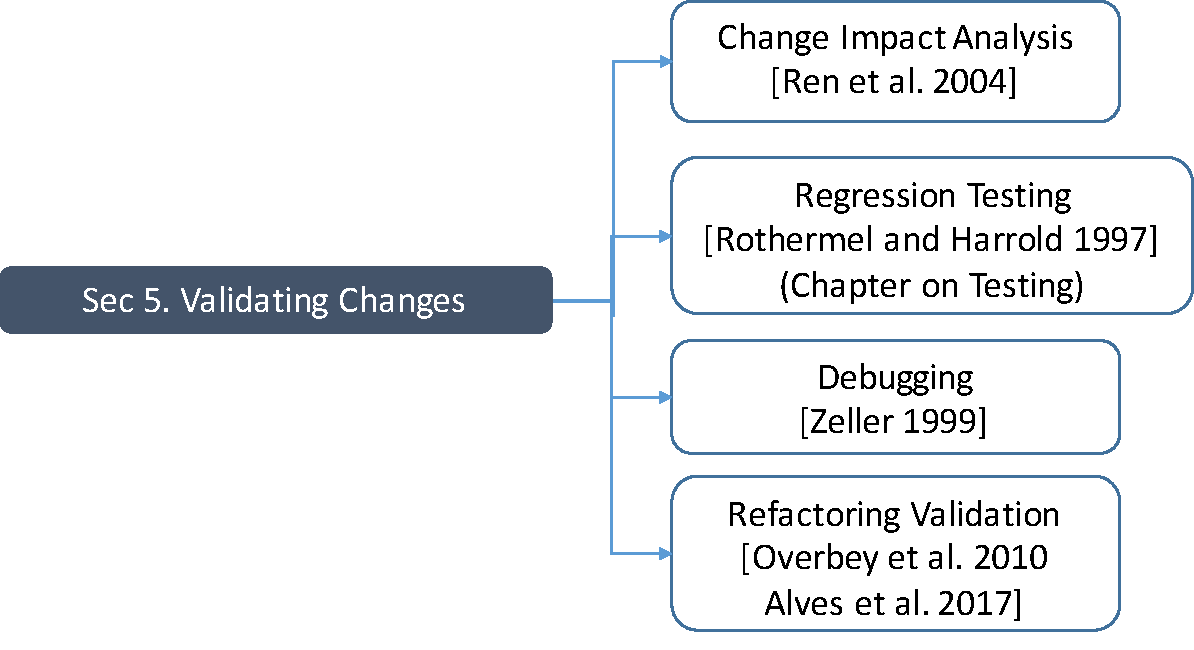
\includegraphics[width=0.6\textwidth]{images/ChangeValidation.pdf} 
 \caption{Change Validation and Related Research Topics} 
 \label{fig:changevalidation} 
\end{figure}

After making software changes, developers must validate the correctness of updated software. Validation and verification is a vast area of research. In this section, we focus on techniques that aim to identify faults introduced due to software changes. As Chapter~\todo{cross reference to testing} discusses the history and seminal work on regression testing in details, we refer the interested readers to that chapter instead. Section~\ref{sec:CIA} discusses Change Impact Analysis, which aims to determine the impact of source code edits on programs under test. Section~\ref{sec:deltadebugging} discusses how to localize program changes responsible for test failures. Section~\ref{sec:refactoringvalidation} discusses the techniques that are specifically designed to validate refactoring edits under the assumption that software's external behavior should not change after refactoring. 

\subsection{Change Impact Analysis} 
\label{sec:CIA} 
Change Impact Analysis consists of a collection of techniques for determining the effects of source code modifications, and can improve programmer productivity by: (i) allowing programmers to experiment with different edits, observe the code fragments that they affect, and use this information to determine which edit to select and/or how to augment test suites, (ii) reducing the amount of time and effort needed in running regression tests, by determining that some tests are guaranteed not to be affected by a given set of changes, and (iii) reducing the amount of time and effort spent in debugging, by determining a safe approximation of the changes responsible for a given test’s failure. 

	In this section, we discuss the seminal change impact analysis work, called Chianti that serve the both purposes of affected test identification and isolation of failure-inducing deltas. 
It uses a two-phase approach in Figure~\ref{fig:twophase}~\cite{Ren2004}. 

\newtext{In the first phase, to identify which test cases a developer must rerun on the new version to ensure that all potential regression faults are identified, Chianti takes the old and new program versions $P_o$ and $P_n$ and an existing test suite $T$ as inputs, and identify a set of atomic program changes at the level of methods, fields, and subtyping relationships. It then computes the profile of the test suite $T$ on $P_o$ in terms of dynamic call graphs and selects $T'\subset T$ that guarantees the same regression fault revealing capability between $T$ and $T'$. }

\newtext{In the second phase, Chianti then first runs the selected test cases $T'$ from the first phase on the new program version $P_n$ and computes the profile of $T'$ on $P_n$ in terms of dynamic call graphs. It then uses both the atomic change set information together with dynamic call graphs to identify which subset of the delta between $P_o$ and $P_n$ led to the behavior differences for each failed test on $P_n$. }

\begin{figure*}
\centering
\begin{minipage}{.45\textwidth}
  \centering
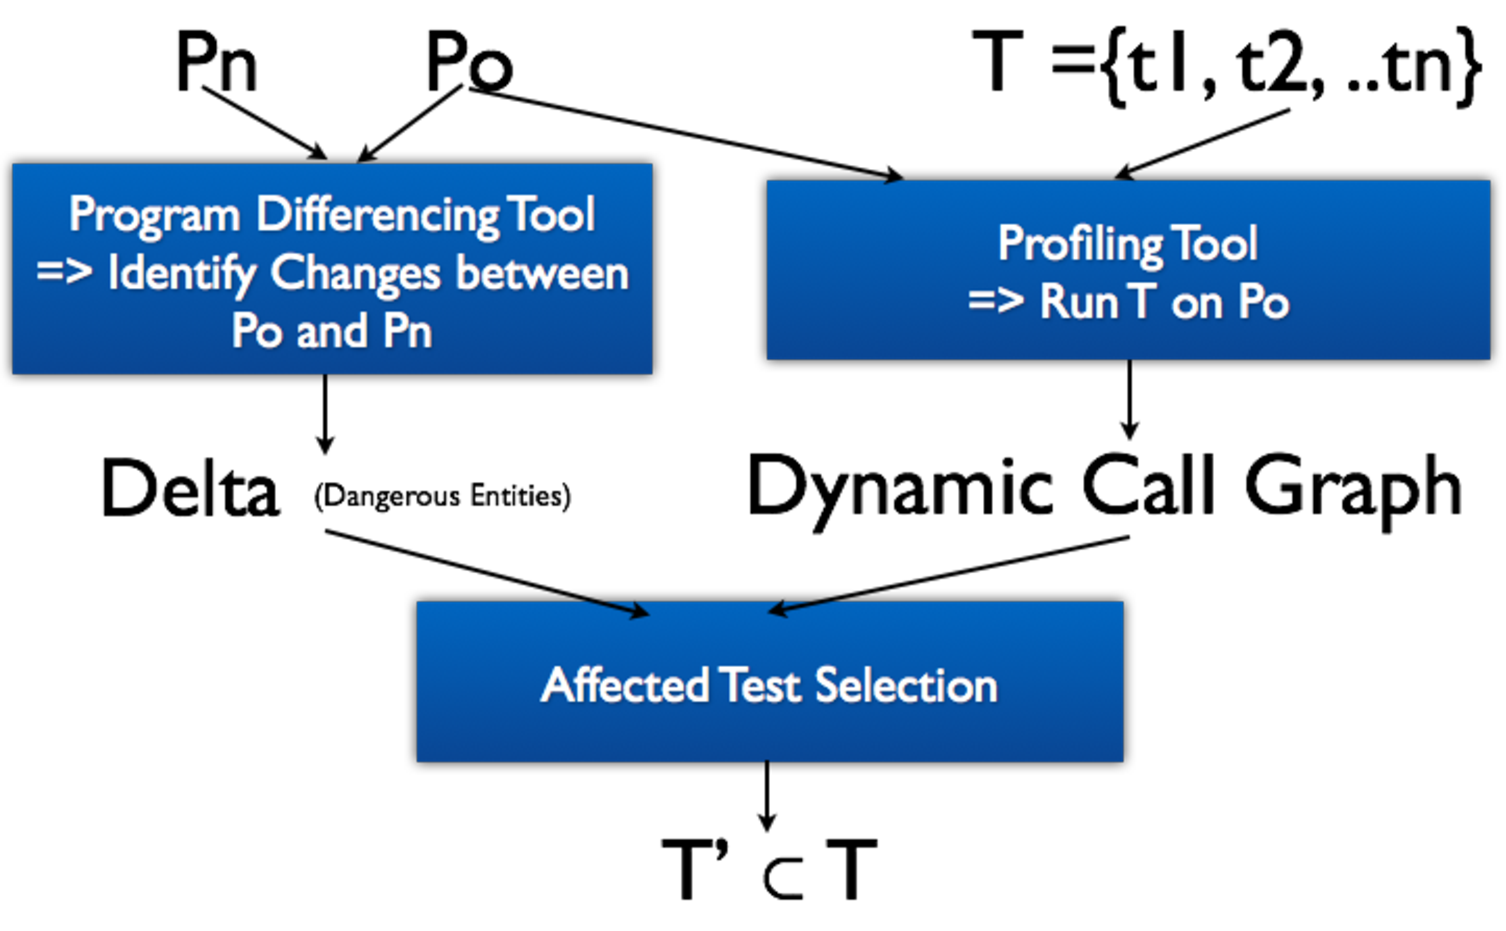
\includegraphics[width=0.9\textwidth]{images/ChiantiPhase1.pdf}
\end{minipage}
\begin{minipage}{.45\textwidth}
  \centering
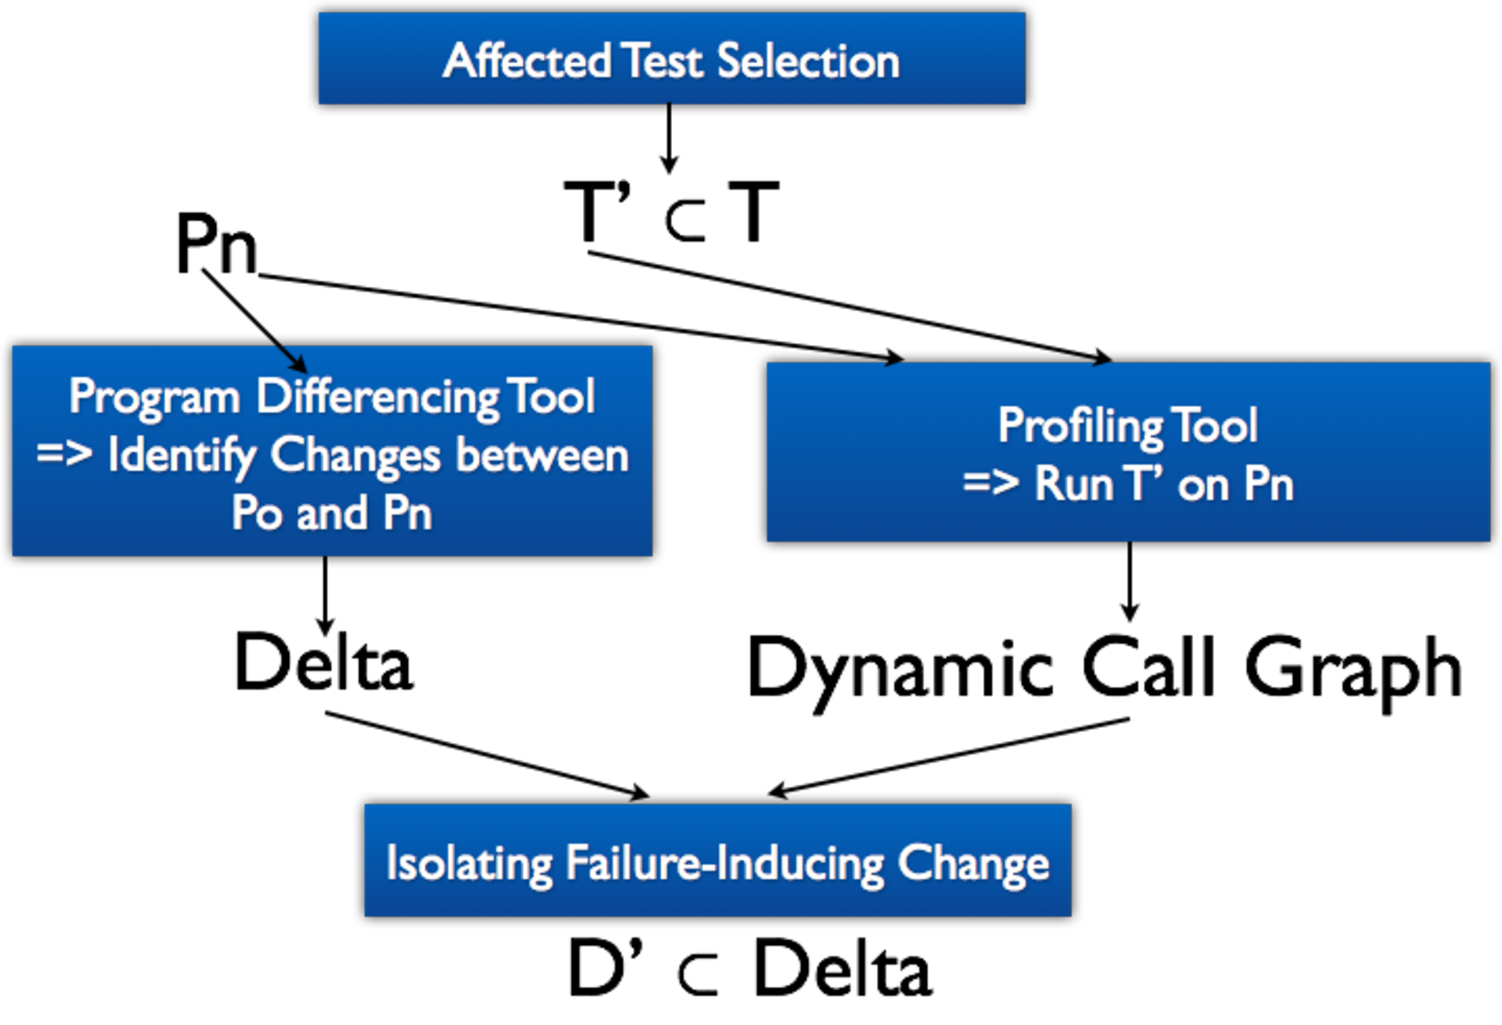
\includegraphics[width=0.9\textwidth]{images/ChiantiPhase2.pdf}
\end{minipage}:w

\caption{Chianti Change Impact Analysis: identifying affected tests (left) and identifying affecting change (right)~\cite{Ren2004}} 
\label{fig:twophase} 
\end{figure*}

\newtext{To represent atomic changes, Chianti compares the syntax tree of the old and new program versions and decomposes the edits into atomic changes at a method and field level. Changes are then categorized as added classes (AC), deleted classes (DC), added methods (AM), deleted methods (DM), changed methods (CM), added fields (AF), deleted fields (DF), and lookup (i.e., dynamic dispatch) changes (LC). The LC atomic change category models changes to the dynamic dispatch behavior of instance methods. In particular, an LC change \codefont{LC(Y, X.m())} models the fact that a call to method \codefont{X.m()} on an object of type \codefont{Y} results in the selection of a different method call target.}

\newtext{For example, Figure~\ref{fig:chianti} shows a software change example and corresponding lists of atomic changes inferred from AST-level comparison. An arrow from an atomic change $A1$ to an atomic change $A2$ indicates that $A2$ is dependent on $A1$. For example, the addition of the call \codefont{B.bar()} in method \codefont{B.foo()} is the method body change \codefont{CM(B.foo())} represented as \textcircled{8}. This change \codefont{8} requires the declaration of method \codefont{B.bar()} to exist first, i.e., \codefont{AM(B.bar())} represented as \textcircled{6}. This dependence is represented as an arrow from \textcircled{6} to \textcircled{8}.}

\newtext{Phase I reports {\bf affected tests}\textemdash a subset of regression tests relevant to edits. It identifies a test if its dynamic call graph on the old version contains a node that corresponds to a changed method (CM) or deleted method (DM)  or or if the call graph contains an edge that corresponds to a lookup change (LC). Figure~\ref{fig:chianti} also shows the dynamic call graph of each test for the old version (left) and the new version (right). Using the call graphs on the left, it is easy to see that: (i) \codefont{test1} is not affected, (ii) \codefont{test2} is affected because its call graph contains a node for \codefont{B.foo()}, which corresponds to \textcircled{8}, and (iii) \codefont{test3} is affected because its call graph contains an edge corresponding to a dispatch to method \codefont{A.foo()} on an object of type \codefont{C}, which corresponds to \textcircled{4}.}

\newtext{Phase II then reports {\bf affecting changes}\textemdash a subset of changes relevant to the execution of affected tests in the new version. For example, we can compute the affecting changes for \codefont{test2} as follows. The call graph for \codefont{test2} in the edited version of the program contains methods \codefont{B.foo()} and \codefont{B.bar()}. These nodes correspond to \textcircled{8} and \textcircled{9} respectively. Atomic change \textcircled{8} requires \textcircled{6} and \textcircled{9} requires \textcircled{6} and \textcircled{7}. Therefore, the atomic changes affecting test2 are \textcircled{6}, \textcircled{7}, \textcircled{8}, and \textcircled{9}. Informally, this means that we can automatically determine that \codefont{test2} is affected by the addition of field \codefont{B.y}, the addition of method \codefont{B.bar()}, and the change to method \codefont{B.foo()}, but not on any of the other source code changes.}

\begin{figure*}
\centering
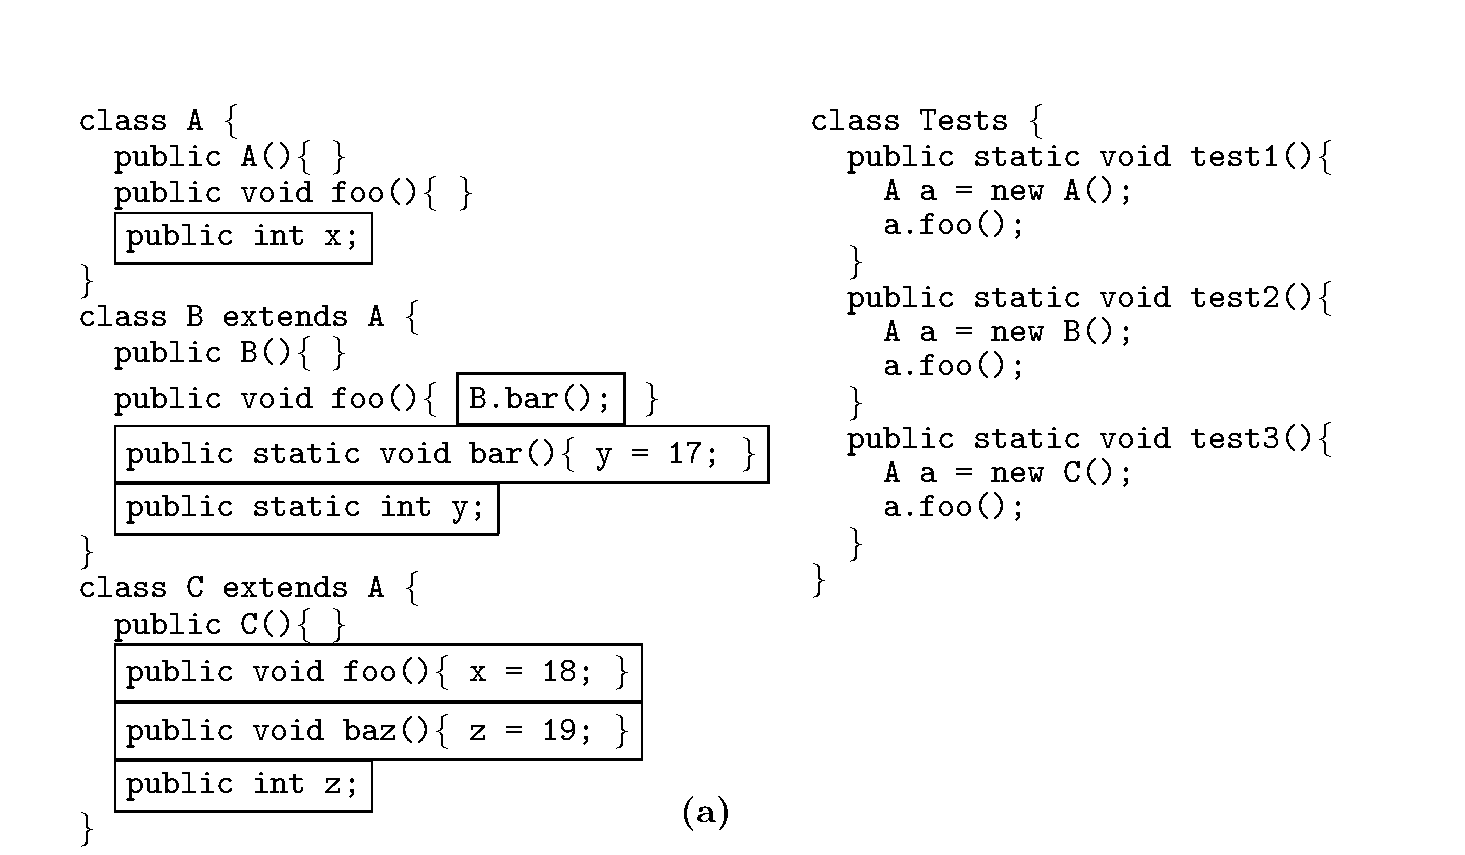
\includegraphics[width=0.95\textwidth]{images/ChiantiExample.pdf}
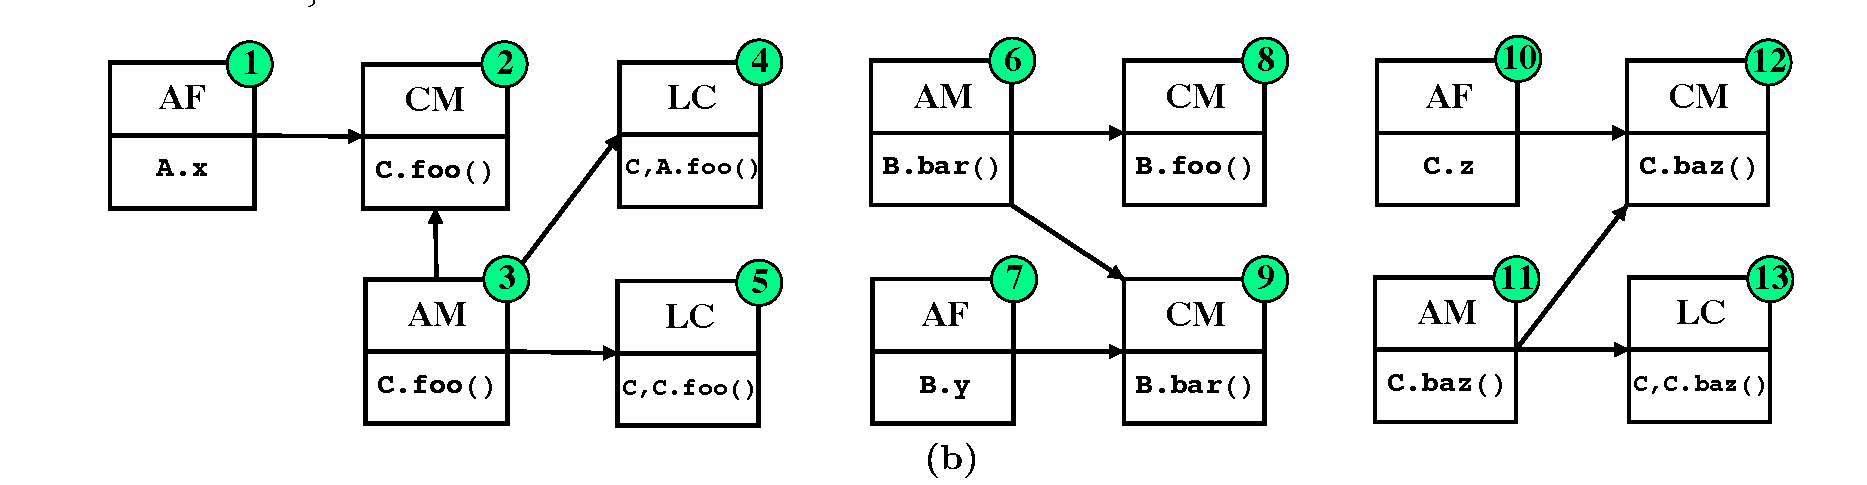
\includegraphics[width=0.95\textwidth]{images/ChiantiAtomicChange.pdf}

\includegraphics[width=0.9\textwidth]{images/DynamicCallGraph.png}
\caption{Chianti change impact analysis} 
\label{fig:chianti} 
\end{figure*}

\subsection{Debugging Changes} 
\label{sec:deltadebugging} 
The problem of simplifying and isolating failure-inducing input is a long standing problem in software engineering. {\it Delta Debugging (DD)} addresses this problem by repetitively running a program with different sub-configurations (subsets) of the input to systematically isolate failure-inducing inputs~\cite{Zeller1999, zeller01}. DD splits the original input into two halves using a binary search-like strategy and re-runs them.  DD requires a test oracle function $test(c)$ that takes an input configuration $c$ and checks whether running a program with $c$ leads to a failure.  If one of the two halves fails, DD recursively applies the same procedure for only that failure-inducing input configuration. On the other hand, if both halves pass, DD tries different sub-configurations by mixing fine-grained sub-configurations with larger sub-configurations (computed as the complement from the current configuration). 

Under the assumption that failure is {\em monotone}\textemdash where $C$ is a super set of all configurations, if a larger configuration $c$ is successful, then any of its smaller sub-configurations $c'$ does not fail, i.e., $\forall c \subset C\ (\ test(c)=\text{\cmark} \rightarrow \forall c' \subset c \  (test(c') \neq$ \ding{55})), DD returns a minimal failure-inducing configuration. %Figure~\ref{fig:deltadebugging} shows the pseudo-code of DD and the illustration of isolating failure-inducing inputs. 

\begin{comment}
\begin{figure*}
\centering
\begin{minipage}{0.9\textwidth}
  \centering
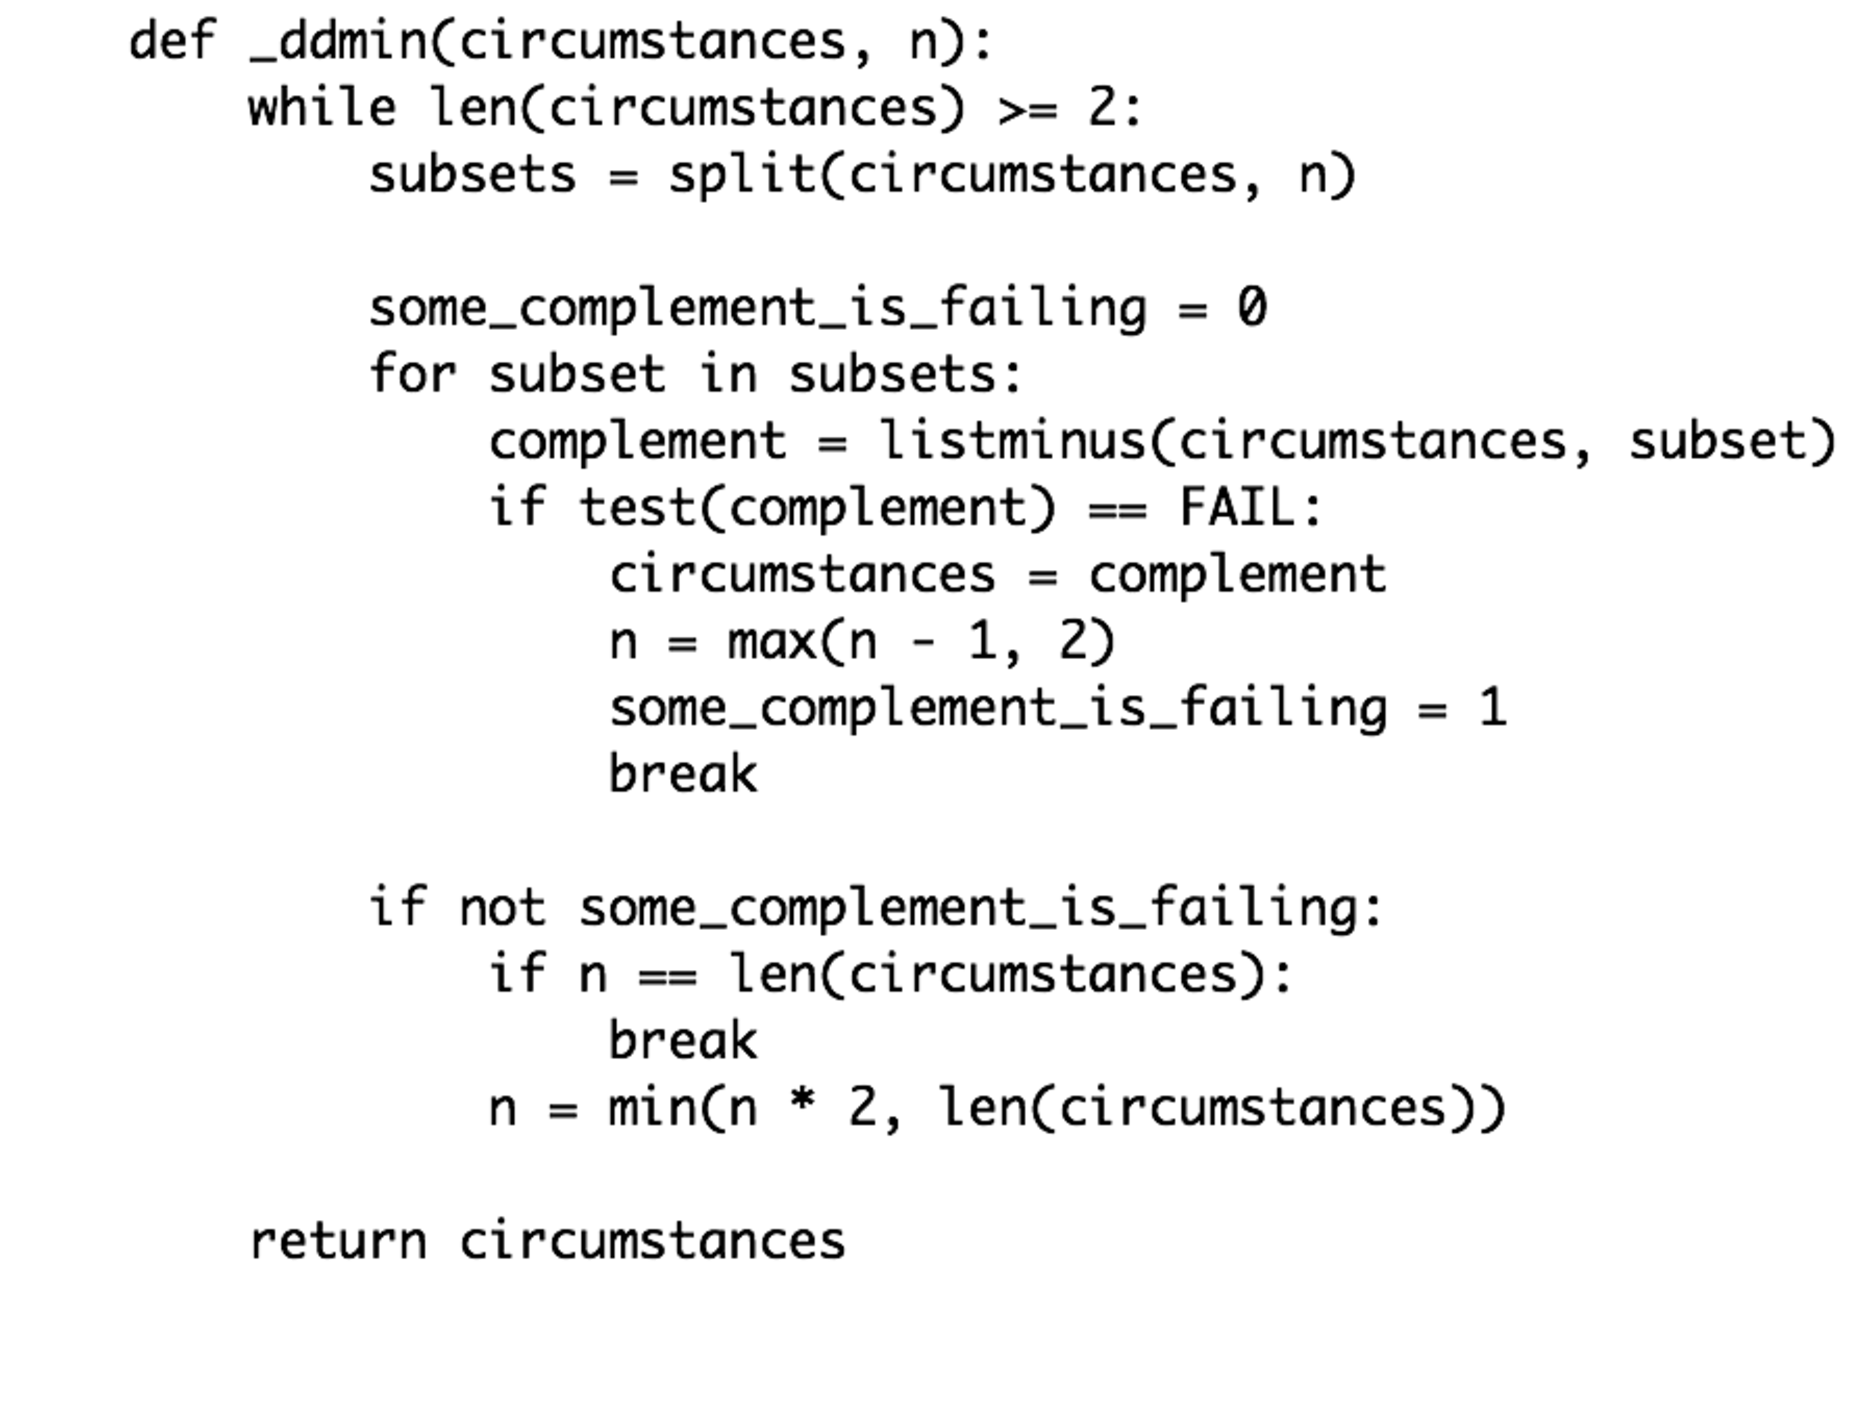
\includegraphics[width=1\textwidth]{images/DeltaDebugging.pdf}
\end{minipage}
\begin{minipage}{0.9\textwidth}
  \centering
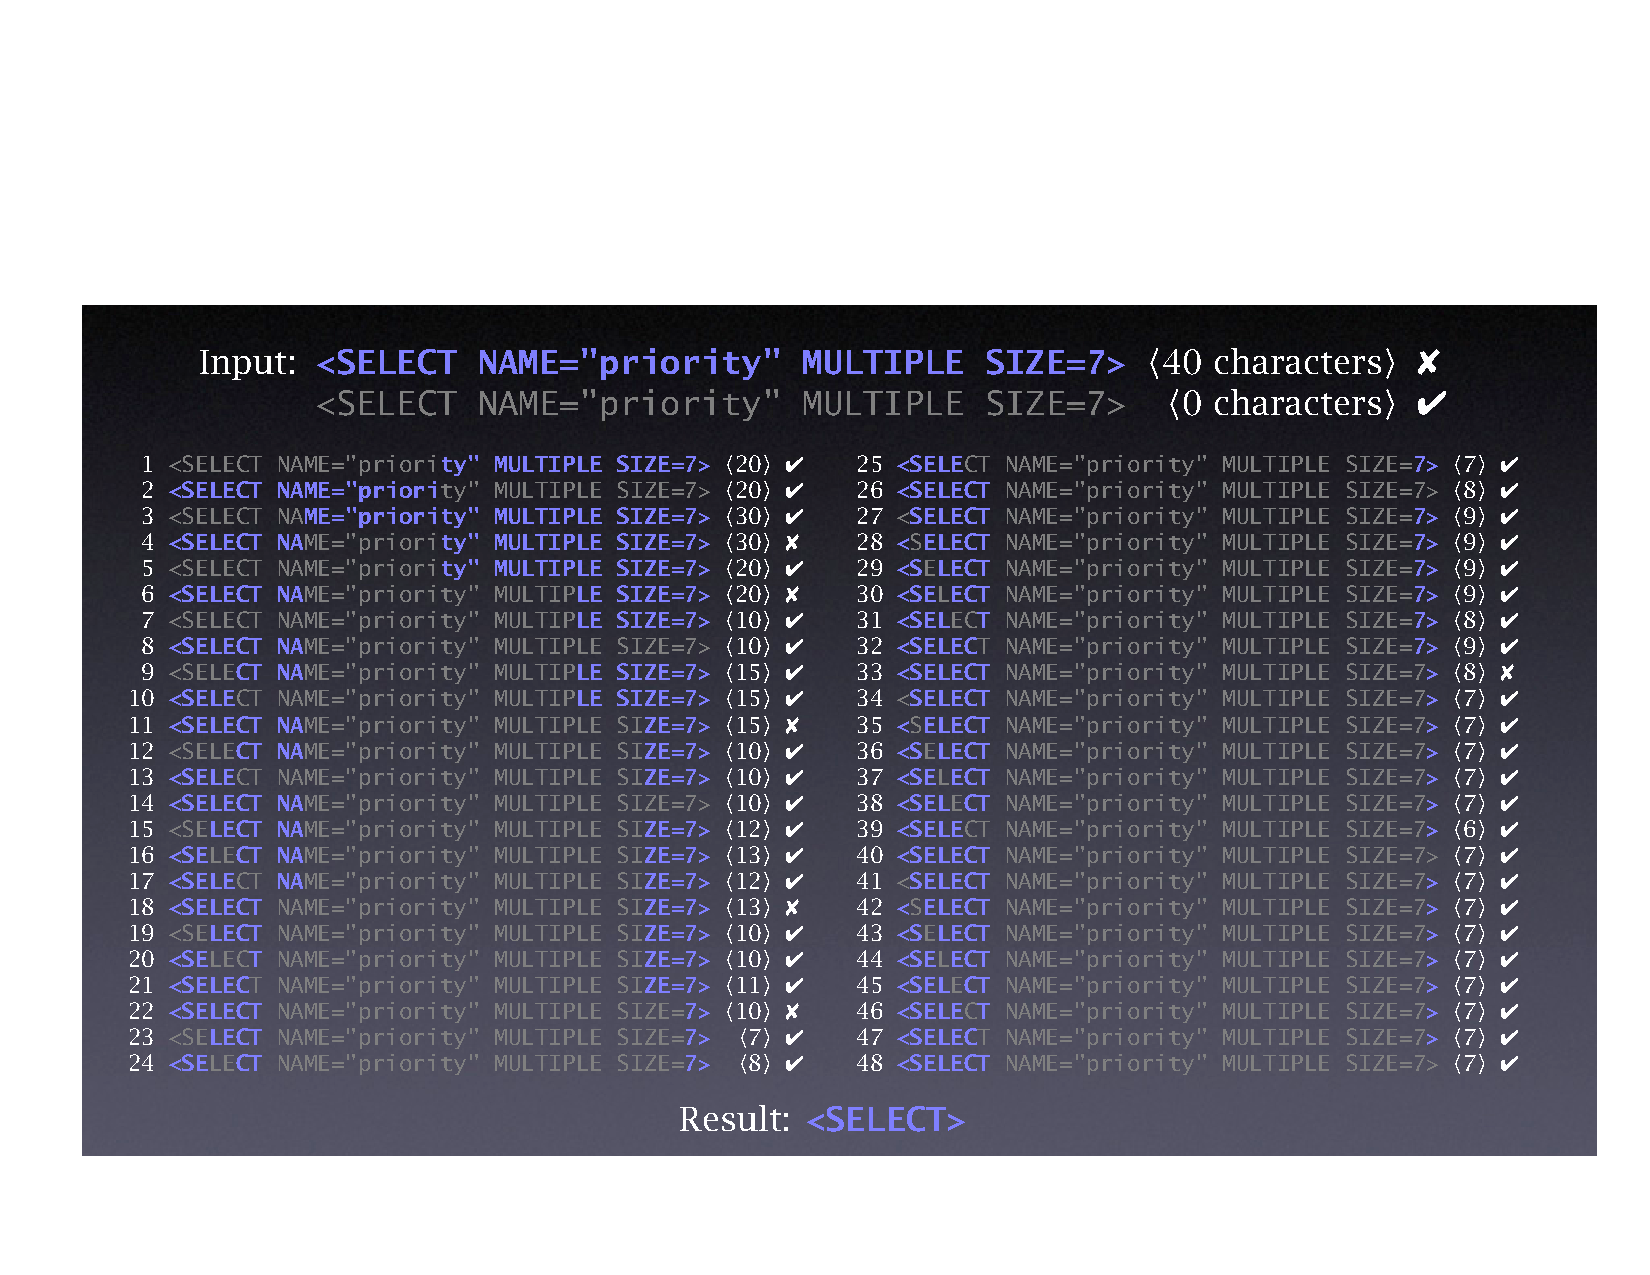
\includegraphics[width=1\textwidth]{images/DeltaDebuggingIlustration.pdf}
\end{minipage}
\caption{Delta Debugging: Algorithm and Illustration} 
\label{fig:deltadebugging} 
\end{figure*}
\end{comment}  

\newtext{This idea of Delta Debugging was applied to isolate failure-inducing changes. It considers all line-level changes between the old and new program version as the candidate set without considering compilation dependences among those changes. In Zeller's seminal paper, {\em ``yesterday, my program worked, but today, it does not, why?''} Zeller demonstrates the application of DD to isolate program edits responsible for regression failures~\cite{Zeller1999}.} DDD 3.1.2, released in December, 1998, exhibited a nasty behavioral change: When invoked with a the name of a non-existing file, DDD 3.1.2 dumped core, while its predecessor DDD 3.1.1 simply gave an error message. The DDD configuration management archive lists 116 logical changes between the 3.1.1 and 3.1.2 releases. These changes were split into 344 textual changes to the DDD source. After only 12 test runs and 58 minutes, the failure-inducing change was found: 
\begin{verbatim}
diff -r1.30 -r1.30.4.1 ddd/gdbinit.C 
295,296c296
<
< --- >
string classpath =
getenv("CLASSPATH") != 0 ? getenv("CLASSPATH") : ".";
string classpath = source view->class path();
\end{verbatim} 

When called with an argument that is not a file name, DDD 3.1.1 checks whether it is a Java class; so DDD consults its environment for the class lookup path. As an ``improvement'', DDD 3.1.2 uses a dedicated method for this purpose. Unfortunately, the source view pointer used is initialized only later, resulting in a core dump. 


\paragraph{Spectra-based fault localization.} Spectrum-based fault localization techniques such as Tarantula~\cite{Jones2002:tarantula} statistically compute suspiciousness scores for statements based on execution traces of both passed and failed test cases, and rank potential faulty statements based on the derived suspiciousness scores. Researchers have also introduced more suspiciousness computation measures to the realm of fault localization for localizing faulty statements~\cite{naish2011model, lo2010comprehensive} and also developed various automated tool-sets which embodies different spectrum-based fault localization techniques~\cite{tarantula-url, janssen2009zoltar}. However, such spectrum-based fault localization techniques are not scalable to large evolving software systems, as they compute spectra on all statements in each program version and do not leverage information about program edits between the old and new versions.

To address this problem, FaultTracer~\cite{zhang2011localizing} combines Chianti-style change impact analysis and Tarantula-style fault localization. To present a ranked list of potential failure-inducing edits, FaultTracer applies a set of spectrum-based ranking techniques to the affecting changes determined by Chianti-style change impact analysis. It uses a new enhanced call graph representation to measure test spectrum information directly for field-level edits and to improve upon the existing Chianti algorithm. The experimental results show that FaultTracer outperforms Chianti in selecting affected tests (slightly better) as well as in determining affecting changes (with an improvement of approximately 20\%). By ranking the affecting changes using spectrum-based profile, it places a real regression fault within a few atomic changes, significantly reducing developers’ effort in inspecting potential failure-inducing changes.

\subsection{Refactoring Validation} 
\label{sec:refactoringvalidation} 

Unlike other types of changes, refactoring validation is a special category of change validation. By definition, refactoring must guarantee behavior preservation and thus the old version's behavior could be compared against the new version's behavior for behavior preservation. Regression testing is the most used strategy for checking refactoring correctness. However, a recent study finds that test suites are often inadequate ~\cite{Rachatasumrit2012:refactortest} and developers may hesitate to initiate or perform refactoring tasks due to inadequate test coverage~\cite{Kim2012:FSR}. Soares et al.~\cite{Soares:icse10} design and implement SafeRefactor that uses randomly generated test suites for detecting refactoring anomalies. 

Formal verification is an alternative for avoiding refactoring anomalies~\cite{Mens2004:SSR}. Some propose rules for guaranteeing semantic preservation~\cite{cornelio2010sound}, use graph rewriting for specifying refactorings~\cite{mens2005formalizing}, or present a collection of refactoring specifications, which guarantee the correctness by construction~\cite{overbey2010collection}. However, these approaches focus on improving the correctness of automated refactoring through formal specifications only. Assuming that developers may apply refactoring manually rather, Schaeffer et al.~validate refactoring edits by comparing data and control dependences between two program versions~\cite{Schaefer2010:refactoring}. 

RefDistiller is a static analysis approach~\cite{Alves2017:refdistiller,Alves:2014:RRA:2635868.2661674} to support the inspection of manual refactorings. It combines two techniques. First, it applies predefined templates to identify potential missed edits during manual refactoring. Second, it leverages an automated refactoring engine to identify extra edits that might be incorrect, helping to  determine the root cause of detected refactoring anomalies. GhostFactor~\cite{geManual2014} checks the correctness of manual refactoring, similar to RefDistiller. Another approach by Ge and Murphy-Hill~\cite{emersoncodereview:2014chase} helps reviewers by identifying applied refactorings and letting developers examine them in isolation by separating pure refactorings. 



 

\section{Future Directions and Open Problems} 

Software maintenance is challenging and time-consuming. Albeit various research and existing tool support, the global cost of debugging software has risen up to \$312 billion annually~\cite{globalcost}. The cost of software maintenance is rising dramatically and has been estimated as more than 90\% of the total cost for software~\cite{Omnext2010}. Software evolution research still has a long future ahead, because there are still challenges and problems that cost developers a lot of time and manual effort. In this section, we highlight some key issues in change comprehension and suggestion.

\subsection{Change Comprehension}
Understanding software changes made by other people is a difficult task, because it requires not only the domain knowledge of the software under maintenance, but also the comprehension of change intent, and the interpretation of mappings between the program semantics of applied changes and those intent. Existing change comprehension and program differencing tools mainly present the textual or syntactical differences between the before- and after- versions of software changes. Current large-scale empirical studies on code changes also focus on textual or syntactical notion of software changes. However, there is no tool support to automatically summarize the semantics of applied changes, or further infer developers' intent behind the changes. 

The new advanced change comprehension tools must assist software professionals in two aspects. First, by summarizing software changes with a natural language description, these tools must produce more meaningful commit messages when developers check in their program changes to software version control systems (e.g., SVN, Git) to facilitate other people (e.g., colleagues and researchers) to mine, comprehend, and analyze applied changes more precisely~\cite{herzig2013impact}. Second, the generated change summary must provide a second opinion to developers of the changes, and enable them to easily check whether the summarized change description matches their actual intent. If there is a mismatch, developers should carefully examine the applied changes and decide whether the changes reflect realize their original intent. 

To design and implement such advanced change comprehension tools, researchers must address several challenges. 
\begin{enumerate}
\item How should we correlate changes applied in source code, configuration files, and databases to present all relevant changes and their relationships as a whole? For instance, how can we explain why a configuration file is changed together with a function's code body? How are the changes in a database schema correspond to source code changes?
\item How should we map concrete code changes or abstract change patterns to natural language descriptions? For instance, when complicated code changes are applied to improve a program's  performance, how can we detect or reveal that intent? How should we differentiate between different types of changes when inferring change intent or producing natural language descriptions accordingly?
\item When developers apply multiple kinds of changes together, such as refactoring some code to facilitate feature addition, we can we identify the boundary between the different types of changes? How can we summarize the changes in a meaningful way so that both types of changes are identified, and the connection between them is characterized clearly? 
\end{enumerate}
To solve these challenges, we may need to invent new program analysis techniques to correlate changes, new change interpretation approaches to characterize different types of changes,
and new text mining and natural language processing techniques to map changes to natural language descriptions.

\subsection{Change Suggestion}
Compared with understanding software changes, applying changes is even more challenging, and can cause serious problems if changes are wrongly applied. Empirical studies showed that 15-70\% of the bug fixes applied during software maintenance were incorrect in their first release~\cite{Sidiroglou:2007:BP,Yin2011:FBB}, which indicates a desperate need for more sophisticated change suggestion tools. 
Below we discuss some of the limitations of existing automatic tool support, and also suggest potential future directions.


\textbf{Corrective Change Suggestion.} Although various tools are proposed to detect different kinds of bugs or even suggest bug fixes, the suggested fixes are usually relatively simple. They may focus on single-line bug fixes, multiple if-condition updates, missing APIs to invoke, or similar code changes that are likely to be applied to similar code snippets. However, no existing approach can suggest a whole missing \codefont{if}-statement or \codefont{while}-loop, neither can they suggest bug fixes that require declaring a new method and inserting the method invocation to appropriate code locations.

\textbf{Adaptive Change Suggestion}. Existing tools allow developers to migrate programs between specific platforms (e.g., desktop and cloud), or support cross-platform software development which enables \textbf{write once, compile anywhere} (WOCA). However, it is not easy to extend these tools when a new platform becomes available and people need to migration programs from existing platforms to the new one. Specifically, 
with the platform-to-platform migration tools, if we have many platforms (e.g., N), theoretically, we need to build and maintain N * (N-1) migration tools to allow the program migration between any two platforms. Although cross-platform software development tools can significantly reduce the necessity of platform-to-platform migration tools, these tools are limited to the platforms for which they are originally built. When a new platform becomes available, these tools will undergo significant modifications to support the new platform. In the future, we need extensible program migration frameworks, which will automatically infer program migration transformations from the concrete migration changes applied by developers, and then apply the inferred transformations to automate other migration tasks for different target platforms. With such frameworks, developers will not need to manually apply repetitive migration changes. 

\textbf{Perfective Change Suggestion}. There are some programming paradigms developed (e.g., AOP and FOP), which facilitate developers to apply perfective changes to enhance or extend any existing software. However, there is no tool support to automatically suggest what perfective changes to apply and where to apply those changes. The main challenge of creating such tools is that unlike other types of changes, perfective changes usually aim to introduce new features instead of modifying existing features. Without any hint provided by developers, it is almost impossible for any tool to predict what new features to add to the software. However, when developers know what new features they want to add but do not know how to implement those features, some advanced tools can be helpful by automatically searching for relevant open source projects, identifying relevant code implementation for the queried features, or even providing customized change suggestion to implement the features and to integrate the features into existing software.

\textbf{Preventive Change Suggestion}.
Although various refactoring tools can automatically refactor code, all the supported refactorings are limited to predefined behavior-preserving program transformations. It is not easy to extend existing refactoring tools to automate new refactorings, especially when the program transformation involves modifications of multiple software entities (i.e., classes, methods, and fields). Some future tools should be designed and implemented to facilitate the extensions of refactoring capabilities.
There are also some refactoring tools that suggest refactoring opportunities based on code smells or software change history. For instance, if there are many code clones in a codebase, existing tools can suggest a clone removal refactoring to reduce duplicated code. In reality, nevertheless, most of the time developers apply refactorings only when they want to apply bug fixes or add new features, which means that refactorings are more likely to be motivated by other kinds of changes instead of code smells and change history~\cite{Silva2016:WWR}. In the future, with the better change comprehension tools mentioned above, we may be able to identify the trends of developers' change intent in the past, and observe how refactorings were applied in combination with other types of changes. Furthermore, with the observed trends, new tools must be built to predict developers' change intent in future, and then suggest refactorings accordingly to prepare for the upcoming changes.


\subsection{Change Validation}
In terms of change validation, there is disproportionately more work being done in the area of validating refactoring (i.e., {\em preventative changes}), compared to other types of changes such as validating {\em adaptive} and {\em perfective} changes. Similarly, in the absence of adequate existing tests which helped to discover defects in the first place, it is not easy to validate whether {\em corrective changes} are applied correctly. 

The reason why is that, with the exception of refactoring that has a canonical, straigthforward definition of {\em behavior preserving modifications}, when it comes to other types of software changes, it is difficult to define the updated semantics of software systems. For example, when a developer adds a new feature, how can we know the desired semantics of the updated software?

This problem naturally brings up the needs of having the specifications of updated software and easier means to write such specifications in the context of software changes. Therefore new tools must be built to guide developers in writing software specifications for the changed parts of the systems. 
and techniques that can effectively leverage the updated specifications to validate different types of software changes. 
In particular, we see a new opportunity for tool support that helps developers in writing updated specifications by suggesting the template for specifications by recognizing the type and pattern of program changes\textemdash are there common specification patterns for each common type of software changes and can we then suggest which specifications to write based on common, frequent types of program modifications such as API evolution? Such tool support must not require developers to write specifications from scratch but rather guide developers on which specific parts of software require new, updated specifications, which parts of software may need additional tests, and how to leverage those written specifications effectively to further guide the remaining areas for writing better specifications. We envision that, with such tool support for reducing the effort of writing specifications for updated software, researchers can build more kinds of debugging and testing techniques that actively leverage those specifications. Such effort will contribute to expansion of change-type specific debugging and testing technologies. 

%\paragraph{Awareness about Software Updates.} 
%enabling programmers to search and filter code changes of interest. 
%supporting investigation and monitoring of program modifications based on the structure, content, and task context of code changes.
%not overload programmers with a large number of change-events or require substantial effort by programmers to specify what they want to monitor. 
%overcome these limitations by automatically inferring awareness-interests and monitoring program changes matching such interests. 
%leverages in-depth automated code change analysis to abstract program differences at a high-level, to determine which subset of changes are refactorings, to reason about {\em interdependence} and {\em interference} among program deltas in order to investigate, search and monitor code changes by their content and structure.  
%leverage automated analysis to help developers manage the impact of other developers' modifications. 


%\paragraph{Awareness about Software Updates.} 
%enabling programmers to search and filter code changes of interest. 
%supporting investigation and monitoring of program modifications based on the structure, content, and task context of code changes.
%not overload programmers with a large number of change-events or require substantial effort by programmers to specify what they want to monitor. 
%overcome these limitations by automatically inferring awareness-interests and monitoring program changes matching such interests. 
%leverages in-depth automated code change analysis to abstract program differences at a high-level, to determine which subset of changes are refactorings, to reason about {\em interdependence} and {\em interference} among program deltas in order to investigate, search and monitor code changes by their content and structure.  
%leverage automated analysis to help developers manage the impact of other developers' modifications. 

 
%Since systematic editing techniques such as LASE automate bug fix pattern inference and when used together with PAR, it could reduce manual effort of similar bug fixes significantly. 
\subsubsection*{Acknowledgments.} 

\section{References}\label{references}
%\bibliography{tianyi,mengna,reference,miryung,kim,refs-kim,refs-wong,kimthesis,libsync,libsync2,chime,faultracer,repair,everton,kimrefactor,rase,spa}
\bibliography{chapter}
\bibliographystyle{abbrv}

\section*{Appendix} 
\end{document}
